\chapter{The Programming Language \textsl{Python}}
We have started our lecture with an introduction to set theory.  In my experience, the notions of
set theory are difficult to master for many students because the concepts introduced in set theory
are quite abstract.  Fortunately, there is a programming language that is suitable to experiment with set
theory and logic.  This is the programming language
\href{https://en.wikipedia.org/wiki/Python_(programming_language)}{Python}, which has its own website at
\href{http://www.python.org}{\texttt{python.org}}.
By programming in \textsl{Python}, students can get acquainted with set theory in a playful manner.
Furthermore, as many interesting problems have a straightforward solution as \textsl{Python} programs,
students can appreciate the usefulness of abstract notions from set theory by programming in \textsl{Python}.
Furthermore, as of 2014 according to 
\href{https://cacm.acm.org/blogs/blog-cacm/176450-python-is-now-the-most-popular-introductory-teaching-language-at-top-u-s-universities/fulltext}{Philip Guo},
8 of the top 10 US universities teach \textsl{Python} in their introductory computer science courses.

The easiest way to install python and its libraries is via \href{https://www.anaconda.com/download/}{Anaconda}.
On many computers, \textsl{Python} is already preinstalled.  Nevertheless, even on those systems it is easiest
to use the \blue{Anaconda} distribution.  The reason is that Anaconda make it very easy to use different
versions of python with different libraries.  In this lecture, we will be using the version 3.6 of \textsl{Python}.

\section{Introductory Examples}
My goal is to introduce \textsl{Python} via a number of rather simple examples.  I will present more
advanced features of \textsl{Python} in later sections, but this section is intended to provide a first
impression of the language.


\begin{figure}[!ht]
\centering
\begin{Verbatim}[ frame         = lines, 
                  framesep      = 0.3cm, 
                  firstnumber   = 1,
                  labelposition = bottomline,
                  numbers       = none,
                  numbersep     = -0.2cm,
                  xleftmargin   = 0.0cm,
                  xrightmargin  = 0.0cm,
                ]
    Python 3.6.4 |Anaconda, Inc.| (default, Jan 16 2018, 12:04:33) 
    [GCC 4.2.1 Compatible Clang 4.0.1 (tags/RELEASE_401/final)] on darwin
    Type "help", "copyright", "credits" or "license" for more information.
    >>> 
\end{Verbatim}
\vspace*{-0.3cm}
\caption{The \textsl{Python} welcome message.}
\label{fig:python}
\end{figure}

The language \textsl{Python} is an \blue{interpreted} language.  Hence, there is no need to \blue{compile} a
program.  Instead, \textsl{Python} programs can be executed via the interpreter.  The interpreter is started
by the command:\footnote{
  While I am usually in the habit of terminating every sentence with either a full stop, a question
  mark or an exclamation mark, I refrain from doing so when the sentence ends in a \textsl{Python} command
  that is shown on a separate line.  The reason is that I want to avoid confusion as it can
  otherwise be hard to understand which part of the line is the command that has to be typed
  verbatim.
}
\\[0.2cm]
\hspace*{1.3cm}
\texttt{python}
\\[0.2cm]
After the interpreter is started, the user sees the output that is shown in Figure 
\ref{fig:python} on page \pageref{fig:python}.  The string
``\texttt{>>>}'' is the \blue{prompt}.  It signals that the interpreter is waiting for input.
If we input the string
\\[0.2cm]
\hspace*{1.3cm}
\texttt{1 + 2}
\\[0.2cm]
and press enter, we get the following output:
\begin{verbatim}
    3
    >>> 
\end{verbatim}
The interpreter has computed the sum $1+2$, returned the result, and prints another prompt waiting
for more input.  Formally, the command ``\texttt{1 + 2}''
is a \blue{script}.  Of course, this is a very small script as it consists only of a single expression.
The command
\\[0.2cm]
\hspace*{1.3cm}
\texttt{exit()}
\\[0.2cm]
terminates the interpreter.   The nice thing about \textsl{Python}  is the we can run \textsl{Python} even in a
browser in so called \href{https://en.wikipedia.org/wiki/Project_Jupyter}{Jupyter notebooks}.  If you have
installed \textsl{Python} by means of the \href{https://www.anaconda.com/download/}{Anaconda} distribution,
then you already have installed Jupyter.  The following subsection  is a the jupyter notebook 
\texttt{Introduction.ipynb}.

\section{\texorpdfstring{An Introduction to
\emph{Python}}{An Introduction to Python}}\label{an-introduction-to-python}

    This \emph{Python} notebook gives a short introduction to \emph{Python}.
We will start with the basics but as the main goal of this introduction
is to show how \emph{Python} supports \emph{sets} we will quickly move
to more advanced topics. In order to show of the features of
\emph{Python} we will give some examples that are not fully explained at
the point where we introduce them. However, rest assured that they will
be explained eventually.

    \subsection{Evaluating expressions}\label{evaluating-expressions}

As Python is an interactive language, expressions can be evaluated
directly. In a \emph{Jupyter} notebook we just have to type Ctrl-Enter
in the cell containing the expression. Instead of Ctrl-Enter we can also
use Shift-Enter.

    \begin{Verbatim}[commandchars=\\\{\}]
{\color{incolor}In [{\color{incolor}1}]:} \PY{l+m+mi}{1} \PY{o}{+} \PY{l+m+mi}{2}
\end{Verbatim}


\begin{Verbatim}[commandchars=\\\{\}]
{\color{outcolor}Out[{\color{outcolor}1}]:} 3
\end{Verbatim}
            
    In \emph{Python}, the precision of integers is not bounded. Hence, the
following expression does not cause an overflow.

    \begin{Verbatim}[commandchars=\\\{\}]
{\color{incolor}In [{\color{incolor}2}]:} \PY{l+m+mi}{1} \PY{o}{*} \PY{l+m+mi}{2} \PY{o}{*} \PY{l+m+mi}{3} \PY{o}{*} \PY{l+m+mi}{4} \PY{o}{*} \PY{l+m+mi}{5} \PY{o}{*} \PY{l+m+mi}{6} \PY{o}{*} \PY{l+m+mi}{7} \PY{o}{*} \PY{l+m+mi}{8} \PY{o}{*} \PY{l+m+mi}{9} \PY{o}{*} \PY{l+m+mi}{10} \PY{o}{*} \PY{l+m+mi}{11} \PY{o}{*} \PY{l+m+mi}{12} \PY{o}{*} \PY{l+m+mi}{13} \PY{o}{*} \PY{l+m+mi}{14} \PY{o}{*} \PY{l+m+mi}{15} \PY{o}{*} \PY{l+m+mi}{16} \PY{o}{*} \PY{l+m+mi}{17} \PY{o}{*} \PY{l+m+mi}{18} \PY{o}{*} \PY{l+m+mi}{19} \PY{o}{*} \PY{l+m+mi}{20} \PY{o}{*} \PY{l+m+mi}{21} \PY{o}{*} \PY{l+m+mi}{22} \PY{o}{*} \PY{l+m+mi}{23} \PY{o}{*} \PY{l+m+mi}{24} \PY{o}{*} \PY{l+m+mi}{25}
\end{Verbatim}


\begin{Verbatim}[commandchars=\\\{\}]
{\color{outcolor}Out[{\color{outcolor}2}]:} 15511210043330985984000000
\end{Verbatim}
            
    The next \emph{cell} in this notebook shows how to compute the
\emph{factorial} of 1000, i.e. it shows how to compute the product
\[ 1000! = 1 * 2 * 3 * \cdots * 998 * 999 * 1000 \] It uses some
advanced features from \emph{functional programming} that will be
discussed at a later stage of this introduction.

    \begin{Verbatim}[commandchars=\\\{\}]
{\color{incolor}In [{\color{incolor}3}]:} \PY{k+kn}{import} \PY{n+nn}{functools} 
        
        \PY{n}{functools}\PY{o}{.}\PY{n}{reduce}\PY{p}{(}\PY{k}{lambda} \PY{n}{x}\PY{p}{,} \PY{n}{y}\PY{p}{:} \PY{p}{(}\PY{n}{x}\PY{o}{*}\PY{n}{y}\PY{p}{)}\PY{p}{,} \PY{n+nb}{range}\PY{p}{(}\PY{l+m+mi}{1}\PY{p}{,} \PY{l+m+mi}{1001}\PY{p}{)}\PY{p}{)}
\end{Verbatim}


\begin{Verbatim}[commandchars=\\\{\}]
{\color{outcolor}Out[{\color{outcolor}3}]:} 402387260077093773543702433923003985719374864210714632543799910429938512398629020592044208486969404800479988610197196058631666872994808558901323829669944590997424504087073759918823627727188732519779505950995276120874975462497043601418278094646496291056393887437886487337119181045825783647849977012476632889835955735432513185323958463075557409114262417474349347553428646576611667797396668820291207379143853719588249808126867838374559731746136085379534524221586593201928090878297308431392844403281231558611036976801357304216168747609675871348312025478589320767169132448426236131412508780208000261683151027341827977704784635868170164365024153691398281264810213092761244896359928705114964975419909342221566832572080821333186116811553615836546984046708975602900950537616475847728421889679646244945160765353408198901385442487984959953319101723355556602139450399736280750137837615307127761926849034352625200015888535147331611702103968175921510907788019393178114194545257223865541461062892187960223838971476088506276862967146674697562911234082439208160153780889893964518263243671616762179168909779911903754031274622289988005195444414282012187361745992642956581746628302955570299024324153181617210465832036786906117260158783520751516284225540265170483304226143974286933061690897968482590125458327168226458066526769958652682272807075781391858178889652208164348344825993266043367660176999612831860788386150279465955131156552036093988180612138558600301435694527224206344631797460594682573103790084024432438465657245014402821885252470935190620929023136493273497565513958720559654228749774011413346962715422845862377387538230483865688976461927383814900140767310446640259899490222221765904339901886018566526485061799702356193897017860040811889729918311021171229845901641921068884387121855646124960798722908519296819372388642614839657382291123125024186649353143970137428531926649875337218940694281434118520158014123344828015051399694290153483077644569099073152433278288269864602789864321139083506217095002597389863554277196742822248757586765752344220207573630569498825087968928162753848863396909959826280956121450994871701244516461260379029309120889086942028510640182154399457156805941872748998094254742173582401063677404595741785160829230135358081840096996372524230560855903700624271243416909004153690105933983835777939410970027753472000000000000000000000000000000000000000000000000000000000000000000000000000000000000000000000000000000000000000000000000000000000000000000000000000000000000000000000000000000000000000000000000000000000000000000000000000000000000000000000000000000000
\end{Verbatim}
            
    The following command will stop the interpreter if executed. It is not
useful inside a \emph{Jupyter} notebook.\\
Hence, the next line should not be evaluated. Therefore, I have put a
comment character "\#" in the first column of this line.

However, if you do remove the comment character and then evaluate the
line, nothing bad will happen as the interpreter is just restarted by
\emph{Jupyter}.

    \begin{Verbatim}[commandchars=\\\{\}]
{\color{incolor}In [{\color{incolor}4}]:} \PY{c+c1}{\PYZsh{} exit()}
\end{Verbatim}


    In order to write something to the screen, we can use the function
print. This function can print objects of any type. In the following
example, this function prints a string. In \emph{Python} any character
sequence enclosed in single quotes is string.

    \begin{Verbatim}[commandchars=\\\{\}]
{\color{incolor}In [{\color{incolor}5}]:} \PY{n+nb}{print}\PY{p}{(}\PY{l+s+s1}{\PYZsq{}}\PY{l+s+s1}{Hello, World!}\PY{l+s+s1}{\PYZsq{}}\PY{p}{)}
\end{Verbatim}


    \begin{Verbatim}[commandchars=\\\{\}]
Hello, World!

    \end{Verbatim}

    Instead of using single quotes we can also use double quotes as seen in
the next example.

    \begin{Verbatim}[commandchars=\\\{\}]
{\color{incolor}In [{\color{incolor}6}]:} \PY{n+nb}{print}\PY{p}{(}\PY{l+s+s2}{\PYZdq{}}\PY{l+s+s2}{Hello, World!}\PY{l+s+s2}{\PYZdq{}}\PY{p}{)}
\end{Verbatim}


    \begin{Verbatim}[commandchars=\\\{\}]
Hello, World!

    \end{Verbatim}

    The function print accepts any number of arguments. For example, to
print the string "36 * 37 / 2 = " followed by the value of the
expression \(36 \cdot 37 / 2\) we can use the following print statement:

    \begin{Verbatim}[commandchars=\\\{\}]
{\color{incolor}In [{\color{incolor}7}]:} \PY{n+nb}{print}\PY{p}{(}\PY{l+s+s2}{\PYZdq{}}\PY{l+s+s2}{36 * 37 / 2 =}\PY{l+s+s2}{\PYZdq{}}\PY{p}{,} \PY{l+m+mi}{36} \PY{o}{*} \PY{l+m+mi}{37} \PY{o}{/}\PY{o}{/} \PY{l+m+mi}{2}\PY{p}{)}
\end{Verbatim}


    \begin{Verbatim}[commandchars=\\\{\}]
36 * 37 / 2 = 666

    \end{Verbatim}

    In the expression "36 * 37 // 2" we have used the operator "//" in order
to enforce \emph{integer division}. If we had used the operator "/"
instead, \emph{Python} would have used \emph{floating point division}
and therefore would have printed the floating point number 666.0 instead
of the integer 666.

    \begin{Verbatim}[commandchars=\\\{\}]
{\color{incolor}In [{\color{incolor}8}]:} \PY{n+nb}{print}\PY{p}{(}\PY{l+s+s2}{\PYZdq{}}\PY{l+s+s2}{36 * 37 / 2 =}\PY{l+s+s2}{\PYZdq{}}\PY{p}{,} \PY{l+m+mi}{36} \PY{o}{*} \PY{l+m+mi}{37} \PY{o}{/} \PY{l+m+mi}{2}\PY{p}{)}
\end{Verbatim}


    \begin{Verbatim}[commandchars=\\\{\}]
36 * 37 / 2 = 666.0

    \end{Verbatim}

    The following script reads a natural number \(n\) and computes the sum
\(\sum\limits_{i=1}^n i\).

\begin{enumerate}
\item The function \texttt{input} prompts the user to enter a string.
\item This string is then converted into an integer using the function \texttt{int}.
\item Next, the \emph{set} \texttt{s} is created such that 
      $$\texttt{s} = \{1, \cdots, n\}. $$  
      The set \texttt{s} is constructed using the function \texttt{range}.  A function call 
      of the form $\texttt{range}(a, b + 1)$ returns a \emph{generator} that produces the natural numbers 
      from $a$ to $b$.  By using this generator as an argument to the function \texttt{set}, a set is created 
      that contains all the natural number starting from $a$ upto and including $b$.
      The precise mechanics of \emph{generators} will be explained later.
\item The \texttt{print} statement uses the function \texttt{sum} to add up all the elements of the
      set \texttt{s}.
\end{enumerate}

    \begin{Verbatim}[commandchars=\\\{\}]
{\color{incolor}In [{\color{incolor}9}]:} \PY{n}{n} \PY{o}{=} \PY{n+nb}{input}\PY{p}{(}\PY{l+s+s1}{\PYZsq{}}\PY{l+s+s1}{Type a natural number and press return: }\PY{l+s+s1}{\PYZsq{}}\PY{p}{)}
        \PY{n}{n} \PY{o}{=} \PY{n+nb}{int}\PY{p}{(}\PY{n}{n}\PY{p}{)}
        \PY{n}{s} \PY{o}{=} \PY{n+nb}{set}\PY{p}{(}\PY{n+nb}{range}\PY{p}{(}\PY{l+m+mi}{1}\PY{p}{,} \PY{n}{n}\PY{o}{+}\PY{l+m+mi}{1}\PY{p}{)}\PY{p}{)}
        \PY{n+nb}{print}\PY{p}{(}\PY{l+s+s1}{\PYZsq{}}\PY{l+s+s1}{The sum 1 + 2 + ... + }\PY{l+s+s1}{\PYZsq{}}\PY{p}{,} \PY{n}{n}\PY{p}{,} \PY{l+s+s1}{\PYZsq{}}\PY{l+s+s1}{ is equal to }\PY{l+s+s1}{\PYZsq{}}\PY{p}{,} \PY{n+nb}{sum}\PY{p}{(}\PY{n}{s}\PY{p}{)}\PY{p}{,} \PY{l+s+s1}{\PYZsq{}}\PY{l+s+s1}{.}\PY{l+s+s1}{\PYZsq{}}\PY{p}{,} \PY{n}{sep}\PY{o}{=} \PY{l+s+s1}{\PYZsq{}}\PY{l+s+s1}{\PYZsq{}}\PY{p}{)}
\end{Verbatim}


    \begin{Verbatim}[commandchars=\\\{\}]
Type a natural number and press return: 36
The sum 1 + 2 + {\ldots} + 36 is equal to 666.

    \end{Verbatim}

    The following example shows how functions can be defined in
\emph{Python}. The function \(\texttt{sum}(n)\) is supposed to compute
the sum of all the numbers in the set \(\{1, \cdots, n\}\). Therefore,
we have \[\texttt{sum}(n) = \sum\limits_{i=1}^n i. \]
The function sum is defined \emph{recursively}. The recursive
implementation of the function sum can best by understood if we observe
that it satisfies the following two equations:
\begin{enumerate}
\item $\texttt{sum}(0) = 0$, 
\item $\texttt{sum}(n) = \texttt{sum}(n-1) + n \quad$  provided that $n > 0$.
\end{enumerate}

    \begin{Verbatim}[commandchars=\\\{\}]
{\color{incolor}In [{\color{incolor}10}]:} \PY{k}{def} \PY{n+nf}{sum}\PY{p}{(}\PY{n}{n}\PY{p}{)}\PY{p}{:}
             \PY{k}{if} \PY{n}{n} \PY{o}{==} \PY{l+m+mi}{0}\PY{p}{:}
                 \PY{k}{return} \PY{l+m+mi}{0}
             \PY{k}{return} \PY{n+nb}{sum}\PY{p}{(}\PY{n}{n}\PY{o}{\PYZhy{}}\PY{l+m+mi}{1}\PY{p}{)} \PY{o}{+} \PY{n}{n}
\end{Verbatim}
 Let us discuss the implementation of the function sum line by line:

\begin{enumerate}
\item The keyword \texttt{def} starts the definition of the function. It is followed by the \emph{name} of the function that is defined.  The name is followed by the list of the \emph{parameters} of the function.  This list is enclosed in parentheses. If there is more than one parameter, the parameters have to be separated by commas.  Finally, there needs to be a colon at the end of the first line.
\item The \emph{body} of the function is indented.  <b>Contrary</b> to most other programming languages, 
     \emph{Python} is \emph{space sensitive}. 
    
     The first statement of the body is a \emph{conditional} statement, which starts with the keyword
     \texttt{if}.  The keyword is followed by a test.  In this case we test whether the variable $n$ 
     is equal to the number $0$.  Note that this test is followed by a colon.
\item The next line contains a \texttt{return} statement.  Note that this statement is again indented.
     All statements indented by the same amount that follow an \texttt{if}-statement are considered as
     the \emph{body} of the \texttt{if}-statement.  In this case the body contains only a single statement.

\item The last line of the function definition contains the recursive invocation of the function \texttt{sum}.
\end{enumerate}

Using the function sum, we can compute the sum \(\sum\limits_{i=1}^n i\)
as follows:

    \begin{Verbatim}[commandchars=\\\{\}]
{\color{incolor}In [{\color{incolor}11}]:} \PY{n}{n}     \PY{o}{=} \PY{n+nb}{int}\PY{p}{(}\PY{n+nb}{input}\PY{p}{(}\PY{l+s+s2}{\PYZdq{}}\PY{l+s+s2}{Enter a natural number: }\PY{l+s+s2}{\PYZdq{}}\PY{p}{)}\PY{p}{)}
         \PY{n}{total} \PY{o}{=} \PY{n+nb}{sum}\PY{p}{(}\PY{n}{n}\PY{p}{)}
         \PY{k}{if} \PY{n}{n} \PY{o}{\PYZgt{}} \PY{l+m+mi}{2}\PY{p}{:}
             \PY{n+nb}{print}\PY{p}{(}\PY{l+s+s2}{\PYZdq{}}\PY{l+s+s2}{0 + 1 + 2 + ... + }\PY{l+s+s2}{\PYZdq{}}\PY{p}{,} \PY{n}{n}\PY{p}{,} \PY{l+s+s2}{\PYZdq{}}\PY{l+s+s2}{ = }\PY{l+s+s2}{\PYZdq{}}\PY{p}{,} \PY{n}{total}\PY{p}{,} \PY{n}{sep}\PY{o}{=}\PY{l+s+s1}{\PYZsq{}}\PY{l+s+s1}{\PYZsq{}}\PY{p}{)}
         \PY{k}{else}\PY{p}{:} 
             \PY{n+nb}{print}\PY{p}{(}\PY{n}{total}\PY{p}{)}
\end{Verbatim}


    \begin{Verbatim}[commandchars=\\\{\}]
Enter a natural number: 100
0 + 1 + 2 + {\ldots} + 100 = 5050

    \end{Verbatim}

    \subsection{\texorpdfstring{Sets in
\emph{Python}}{Sets in Python}}\label{sets-in-python}

    One of the big deals about \emph{Python} is that \emph{Python} supports
sets as a \textbf{native} datatype. This is one of the reasons that have
lead me to choose \emph{Python} as the programming language for this
course. To get a first impression how sets are handled in \emph{Python},
let us define two simple sets \(A\) and \(B\) and print them:

    \begin{Verbatim}[commandchars=\\\{\}]
{\color{incolor}In [{\color{incolor}12}]:} \PY{n}{A} \PY{o}{=} \PY{p}{\PYZob{}}\PY{l+m+mi}{1}\PY{p}{,} \PY{l+m+mi}{2}\PY{p}{,} \PY{l+m+mi}{3}\PY{p}{\PYZcb{}}
         \PY{n}{B} \PY{o}{=} \PY{p}{\PYZob{}}\PY{l+m+mi}{2}\PY{p}{,} \PY{l+m+mi}{3}\PY{p}{,} \PY{l+m+mi}{4}\PY{p}{\PYZcb{}}
         \PY{n+nb}{print}\PY{p}{(}\PY{l+s+s1}{\PYZsq{}}\PY{l+s+s1}{A = }\PY{l+s+s1}{\PYZsq{}}\PY{p}{,} \PY{n}{A}\PY{p}{,} \PY{l+s+s1}{\PYZsq{}}\PY{l+s+s1}{, B = }\PY{l+s+s1}{\PYZsq{}}\PY{p}{,} \PY{n}{B}\PY{p}{,} \PY{n}{sep}\PY{o}{=}\PY{l+s+s1}{\PYZsq{}}\PY{l+s+s1}{\PYZsq{}}\PY{p}{)}
\end{Verbatim}


    \begin{Verbatim}[commandchars=\\\{\}]
A = \{1, 2, 3\}, B = \{2, 3, 4\}

    \end{Verbatim}

    The last argument sep='' prevents the print statement from separating
its arguments with space characters.

There is a caveat here, we cannot define the empty set using the
expression \{\} since this expression creates the empty
\emph{dictionary} instead. (We will discuss the data type of
\emph{dictionaries} later.) To define the empty set, we therefore have
to use the following expression:

    \begin{Verbatim}[commandchars=\\\{\}]
{\color{incolor}In [{\color{incolor}13}]:} \PY{n+nb}{set}\PY{p}{(}\PY{p}{)}
\end{Verbatim}


\begin{Verbatim}[commandchars=\\\{\}]
{\color{outcolor}Out[{\color{outcolor}13}]:} set()
\end{Verbatim}
            
    Note that the empty set is also printed as set() in \emph{Python} and
not as \{\}.

    Next, let us compute the union \(A \cup B\). This is done using the
function union.

    \begin{Verbatim}[commandchars=\\\{\}]
{\color{incolor}In [{\color{incolor}14}]:} \PY{n}{A}\PY{o}{.}\PY{n}{union}\PY{p}{(}\PY{n}{B}\PY{p}{)}
\end{Verbatim}


\begin{Verbatim}[commandchars=\\\{\}]
{\color{outcolor}Out[{\color{outcolor}14}]:} \{1, 2, 3, 4\}
\end{Verbatim}
            
    As the function union really acts like a \emph{method}, you might
suspect that it does change its first argument. Fortunately, this is not
the case, \(A\) is unchanged as you can see in the next line:

    \begin{Verbatim}[commandchars=\\\{\}]
{\color{incolor}In [{\color{incolor}15}]:} \PY{n}{A}
\end{Verbatim}


\begin{Verbatim}[commandchars=\\\{\}]
{\color{outcolor}Out[{\color{outcolor}15}]:} \{1, 2, 3\}
\end{Verbatim}
            
    To compute the intersection \(A \cap B\), we use the function
intersection:

    \begin{Verbatim}[commandchars=\\\{\}]
{\color{incolor}In [{\color{incolor}16}]:} \PY{n}{A}\PY{o}{.}\PY{n}{intersection}\PY{p}{(}\PY{n}{B}\PY{p}{)}
\end{Verbatim}


\begin{Verbatim}[commandchars=\\\{\}]
{\color{outcolor}Out[{\color{outcolor}16}]:} \{2, 3\}
\end{Verbatim}
            
    Again \(A\) is not changed.

    \begin{Verbatim}[commandchars=\\\{\}]
{\color{incolor}In [{\color{incolor}17}]:} \PY{n}{A}
\end{Verbatim}


\begin{Verbatim}[commandchars=\\\{\}]
{\color{outcolor}Out[{\color{outcolor}17}]:} \{1, 2, 3\}
\end{Verbatim}
            
    The difference \(A \backslash B\) is computed using the operator "-":

    \begin{Verbatim}[commandchars=\\\{\}]
{\color{incolor}In [{\color{incolor}18}]:} \PY{n}{A} \PY{o}{\PYZhy{}} \PY{n}{B}
\end{Verbatim}


\begin{Verbatim}[commandchars=\\\{\}]
{\color{outcolor}Out[{\color{outcolor}18}]:} \{1\}
\end{Verbatim}
            
    It is easy to test whether \(A \subseteq B\) holds:

    \begin{Verbatim}[commandchars=\\\{\}]
{\color{incolor}In [{\color{incolor}19}]:} \PY{n}{A} \PY{o}{\PYZlt{}}\PY{o}{=} \PY{n}{B}
\end{Verbatim}


\begin{Verbatim}[commandchars=\\\{\}]
{\color{outcolor}Out[{\color{outcolor}19}]:} False
\end{Verbatim}
            
    Testing whether an object \(x\) is an element of a set \(M\), i.e. to
test, whether \(x \in M\) holds is straightforward:

    \begin{Verbatim}[commandchars=\\\{\}]
{\color{incolor}In [{\color{incolor}20}]:} \PY{l+m+mi}{1} \PY{o+ow}{in} \PY{n}{A}
\end{Verbatim}


\begin{Verbatim}[commandchars=\\\{\}]
{\color{outcolor}Out[{\color{outcolor}20}]:} True
\end{Verbatim}
            
    On the other hand, the number \(1\) is not an element of the set \(B\),
i.e. we have \(1 \not\in B\):

    \begin{Verbatim}[commandchars=\\\{\}]
{\color{incolor}In [{\color{incolor}21}]:} \PY{l+m+mi}{1} \PY{o+ow}{not} \PY{o+ow}{in} \PY{n}{B}
\end{Verbatim}


\begin{Verbatim}[commandchars=\\\{\}]
{\color{outcolor}Out[{\color{outcolor}21}]:} True
\end{Verbatim}
            
    \subsection{Defining Sets via Selection and
Images}\label{defining-sets-via-selection-and-images}
Remember that we can define subsets of a given set \(M\) via the axiom of
selection. If \(p\) is a property such that for any object \(x\) from
the set \(M\) the expression \(p(x)\) is either True or False, the
subset of all those elements of \(M\) such that \(p(x)\) is True can be
defined as \[ \{ x \in M \mid p(x) \}. \] For example, if \(M\) is the
set \(\{1, \cdots, 100\}\) and we want to compute the subset of this set
that contains all numbers from \(M\) that are divisible by \(7\), then
this set can be defined as 
\[ \{ x \in M \mid x \texttt{\%} 7 == 0 \}. \]
In \emph{Python}, the definition of this set can be given as follows:

    \begin{Verbatim}[commandchars=\\\{\}]
{\color{incolor}In [{\color{incolor}22}]:} \PY{n}{M} \PY{o}{=} \PY{n+nb}{set}\PY{p}{(}\PY{n+nb}{range}\PY{p}{(}\PY{l+m+mi}{1}\PY{p}{,} \PY{l+m+mi}{101}\PY{p}{)}\PY{p}{)}
         \PY{p}{\PYZob{}} \PY{n}{x} \PY{k}{for} \PY{n}{x} \PY{o+ow}{in} \PY{n}{M} \PY{k}{if} \PY{n}{x} \PY{o}{\PYZpc{}} \PY{l+m+mi}{7} \PY{o}{==} \PY{l+m+mi}{0} \PY{p}{\PYZcb{}}
\end{Verbatim}


\begin{Verbatim}[commandchars=\\\{\}]
{\color{outcolor}Out[{\color{outcolor}22}]:} \{7, 14, 21, 28, 35, 42, 49, 56, 63, 70, 77, 84, 91, 98\}
\end{Verbatim}
            
    In general, in \emph{Python} the set \[ \{ x \in M \mid p(x) \} \] is
computed by the expression
\[ \{\; x\; \texttt{for}\; x\; \texttt{in}\; M\; \texttt{if}\; p(x)\; \}. \]
\emph{Image} sets can be computed in a similar way. If \(f\) is a
function defined for all elements of a set \(M\), the image set
\[ \{ f(x) \mid x \in M \} \] can be computed in \emph{Python} as
follows: \[ \{\; f(x)\; \texttt{for}\; x\; \texttt{in}\; M\; \}. \] For
example, the following expression computes the set of all squares of
numbers from the set \(\{1,\cdots,10\}\):

    \begin{Verbatim}[commandchars=\\\{\}]
{\color{incolor}In [{\color{incolor}23}]:} \PY{n}{M} \PY{o}{=} \PY{n+nb}{set}\PY{p}{(}\PY{n+nb}{range}\PY{p}{(}\PY{l+m+mi}{1}\PY{p}{,}\PY{l+m+mi}{11}\PY{p}{)}\PY{p}{)}
         \PY{p}{\PYZob{}} \PY{n}{x}\PY{o}{*}\PY{n}{x} \PY{k}{for} \PY{n}{x} \PY{o+ow}{in} \PY{n}{M} \PY{p}{\PYZcb{}}
\end{Verbatim}


\begin{Verbatim}[commandchars=\\\{\}]
{\color{outcolor}Out[{\color{outcolor}23}]:} \{1, 4, 9, 16, 25, 36, 49, 64, 81, 100\}
\end{Verbatim}
            
The computation of image sets and selections can be combined. If \(M\)
is a set, \(p\) is a property such taht \(p(x)\) is either True or False
for elements of \(M\), and \(f\) is a function such that \(f(x)\) is
defined for all \(x \in M\) then we can compute set
\[ \{ f(x) \mid  x \in M \wedge p(x) \} \] of all images \(f(x)\) from
those \(x\in M\) that satisfy the property \(p(x)\) via the expression
\[ \{\; f(x)\; \texttt{for}\; x\; \texttt{in}\; M\; \texttt{if}\; p(x)\; \}. \]
For example, to compute the set of those squares of numbers from the set
\(\{1,\cdots,10\}\) that are even we can write

    \begin{Verbatim}[commandchars=\\\{\}]
{\color{incolor}In [{\color{incolor}24}]:} \PY{n}{M} \PY{o}{=} \PY{n+nb}{set}\PY{p}{(}\PY{n+nb}{range}\PY{p}{(}\PY{l+m+mi}{1}\PY{p}{,}\PY{l+m+mi}{11}\PY{p}{)}\PY{p}{)}
         \PY{p}{\PYZob{}} \PY{n}{x}\PY{o}{*}\PY{n}{x} \PY{k}{for} \PY{n}{x} \PY{o+ow}{in} \PY{n}{M} \PY{k}{if} \PY{n}{x} \PY{o}{\PYZpc{}} \PY{l+m+mi}{2} \PY{o}{==} \PY{l+m+mi}{0} \PY{p}{\PYZcb{}}
\end{Verbatim}


\begin{Verbatim}[commandchars=\\\{\}]
{\color{outcolor}Out[{\color{outcolor}24}]:} \{4, 16, 36, 64, 100\}
\end{Verbatim}
            
    We can iterate over more than one set. For example, let us define the
set of all products \(p \cdot q\) of numbers \(p\) and \(q\) from the
set \(\{2, \cdots, 10\}\), i.e. we intend to define the set
\[ \bigl\{ p \cdot q \bigm| p \in \{2,\cdots,10\} \wedge q \in \{2,\cdots,10\} \bigr\}. \]
In \emph{Python}, this set is defined as follows:

    \begin{Verbatim}[commandchars=\\\{\}]
{\color{incolor}In [{\color{incolor}25}]:} \PY{n+nb}{print}\PY{p}{(}\PY{p}{\PYZob{}} \PY{n}{p} \PY{o}{*} \PY{n}{q} \PY{k}{for} \PY{n}{p} \PY{o+ow}{in} \PY{n+nb}{range}\PY{p}{(}\PY{l+m+mi}{2}\PY{p}{,}\PY{l+m+mi}{11}\PY{p}{)} \PY{k}{for} \PY{n}{q} \PY{o+ow}{in} \PY{n+nb}{range}\PY{p}{(}\PY{l+m+mi}{2}\PY{p}{,}\PY{l+m+mi}{11}\PY{p}{)} \PY{p}{\PYZcb{}}\PY{p}{)}
\end{Verbatim}


    \begin{Verbatim}[commandchars=\\\{\}]
\{4, 6, 8, 9, 10, 12, 14, 15, 16, 18, 20, 21, 24, 25, 27, 28, 30, 32, 35, 36, 40, 42, 45, 48, 49, 50, 54, 56, 60, 63, 64, 70, 72, 80, 81, 90, 100\}

    \end{Verbatim}

    We can use this set to compute the set of \emph{prime numbers}. After
all, the set of prime numbers is the set of all those natural numbers
bigger than \(1\) that can not be written as a proper product, that is a
number \(x\) is \emph{prime} if

\begin{enumerate}
\item $x$ is bigger than $1$ and 
\item there are no natural numbers $x$ and $y$ both bigger than $1$ such that $x = p * q$ holds.
\end{enumerate}

More formally, the set \(\mathbb{P}\) of prime numbers is defined as
follows:
\[ \mathbb{P} = \bigl\{ x \in \mathbb{N} \;\bigm|\; x > 1 \wedge \neg \exists p, q \in \mathbb{N}: (x = p * q \wedge p > 1 \wedge q > 1)\bigr\}. \]
Hence the following code computes the set of all primes less than 100:

    \begin{Verbatim}[commandchars=\\\{\}]
{\color{incolor}In [{\color{incolor}26}]:} \PY{n}{s} \PY{o}{=} \PY{n+nb}{set}\PY{p}{(}\PY{n+nb}{range}\PY{p}{(}\PY{l+m+mi}{2}\PY{p}{,}\PY{l+m+mi}{100}\PY{p}{)}\PY{p}{)}
         \PY{n+nb}{print}\PY{p}{(}\PY{n}{s} \PY{o}{\PYZhy{}} \PY{p}{\PYZob{}} \PY{n}{p} \PY{o}{*} \PY{n}{q} \PY{k}{for} \PY{n}{p} \PY{o+ow}{in} \PY{n}{s} \PY{k}{for} \PY{n}{q} \PY{o+ow}{in} \PY{n}{s} \PY{p}{\PYZcb{}}\PY{p}{)}
\end{Verbatim}


    \begin{Verbatim}[commandchars=\\\{\}]
\{2, 3, 5, 7, 11, 13, 17, 19, 23, 29, 31, 37, 41, 43, 47, 53, 59, 61, 67, 71, 73, 79, 83, 89, 97\}

    \end{Verbatim}

    An alternative way to compute primes works by noting that a number \(p\)
is prime iff there is no number \(t\) other than \(1\) and \(p\) that
divides the number \(p\). The function dividers given below computes the
set of all numbers dividing a given number \(p\) evenly:

    \begin{Verbatim}[commandchars=\\\{\}]
{\color{incolor}In [{\color{incolor}27}]:} \PY{k}{def} \PY{n+nf}{dividers}\PY{p}{(}\PY{n}{p}\PY{p}{)}\PY{p}{:}
             \PY{l+s+s2}{\PYZdq{}}\PY{l+s+s2}{Compute the set of numbers that divide the number p.}\PY{l+s+s2}{\PYZdq{}}
             \PY{k}{return} \PY{p}{\PYZob{}} \PY{n}{t} \PY{k}{for} \PY{n}{t} \PY{o+ow}{in} \PY{n+nb}{range}\PY{p}{(}\PY{l+m+mi}{1}\PY{p}{,} \PY{n}{p}\PY{o}{+}\PY{l+m+mi}{1}\PY{p}{)} \PY{k}{if} \PY{n}{p} \PY{o}{\PYZpc{}} \PY{n}{t} \PY{o}{==} \PY{l+m+mi}{0} \PY{p}{\PYZcb{}}
         
         \PY{n}{n}      \PY{o}{=} \PY{l+m+mi}{100}\PY{p}{;}
         \PY{n}{primes} \PY{o}{=} \PY{p}{\PYZob{}} \PY{n}{p} \PY{k}{for} \PY{n}{p} \PY{o+ow}{in} \PY{n+nb}{range}\PY{p}{(}\PY{l+m+mi}{2}\PY{p}{,} \PY{n}{n}\PY{p}{)} \PY{k}{if} \PY{n}{dividers}\PY{p}{(}\PY{n}{p}\PY{p}{)} \PY{o}{==} \PY{p}{\PYZob{}}\PY{l+m+mi}{1}\PY{p}{,} \PY{n}{p}\PY{p}{\PYZcb{}} \PY{p}{\PYZcb{}}
         \PY{n+nb}{print}\PY{p}{(}\PY{n}{primes}\PY{p}{)}
\end{Verbatim}


    \begin{Verbatim}[commandchars=\\\{\}]
\{2, 3, 5, 7, 11, 13, 17, 19, 23, 29, 31, 37, 41, 43, 47, 53, 59, 61, 67, 71, 73, 79, 83, 89, 97\}

    \end{Verbatim}

    \subsection{Computing the Power Set}\label{computing-the-power-set}

    Unfortunately, there is no operator to compute the power set \(2^M\) of
a given set \(M\). Since the power set is needed frequently, we have to
implement a function power to compute this set ourselves. The easiest
way to compute the power set \(2^M\) of a set \(M\) is to implement the
following recursive equations:

\begin{enumerate}
\item The power set of the empty set contains only the empty set:
    $$2^{\{\}} = \bigl\{\{\}\bigr\}$$</li>
\item If a set $M$ can be written as $M = C \cup \{x\}$, where the element $x$ does not occur in the set $C$, then the power set $2^M$ consists of two sets:
      \begin{itemize}
        \item Firstly, all subsets of $C$ are also subsets of $M$.</li>
        \item Secondly, if A is a subset of $C$, then the set $A \cup\{x\}$ is also a subset of $M$.</li>
      \end{itemize}
    If we combine these parts we get the following equation:
    $$2^{C \cup \{x\}} = 2^C \cup \bigl\{ A \cup \{x\} \bigm| A \in 2^C \bigr\}$$
\end{enumerate}

But there is another problem: In \emph{Python} we can't create a set
that has elements that are sets themselves! The reason is that in
\emph{Python} sets are implemented via \emph{hash tables} and therefore
the elements of a set need to be \emph{hashable}. (The notion of an
element being \emph{hashable} will be discussed in more detail in the
lecture on \emph{Algorithms}.) However, sets are \emph{mutable} and
\emph{mutable} objects are not \emph{hashable}. Fortunately, there is a
workaround: \emph{Python} provides the data type of \emph{frozen sets}.
These sets behave like sets but are are lacking certain function and
hence are unmutable. So if we use \emph{frozen sets} as elements of the
power set, we can compute the power set of a given set. The function
power given below shows how this works.

    \begin{Verbatim}[commandchars=\\\{\}]
{\color{incolor}In [{\color{incolor}28}]:} \PY{k}{def} \PY{n+nf}{power}\PY{p}{(}\PY{n}{M}\PY{p}{)}\PY{p}{:}
             \PY{l+s+s2}{\PYZdq{}}\PY{l+s+s2}{This function computes the power set of the set M.}\PY{l+s+s2}{\PYZdq{}}
             \PY{k}{if} \PY{n}{M} \PY{o}{==} \PY{n+nb}{set}\PY{p}{(}\PY{p}{)}\PY{p}{:}
                 \PY{k}{return} \PY{p}{\PYZob{}} \PY{n+nb}{frozenset}\PY{p}{(}\PY{p}{)} \PY{p}{\PYZcb{}}
             \PY{k}{else}\PY{p}{:}
                 \PY{n}{C}  \PY{o}{=} \PY{n+nb}{set}\PY{p}{(}\PY{n}{M}\PY{p}{)}  \PY{c+c1}{\PYZsh{} C is a copy of M as we don\PYZsq{}t want to change the set M}
                 \PY{n}{x}  \PY{o}{=} \PY{n}{C}\PY{o}{.}\PY{n}{pop}\PY{p}{(}\PY{p}{)} \PY{c+c1}{\PYZsh{} pop removes the element x from the set C}
                 \PY{n}{P1} \PY{o}{=} \PY{n}{power}\PY{p}{(}\PY{n}{C}\PY{p}{)}
                 \PY{n}{P2} \PY{o}{=} \PY{p}{\PYZob{}} \PY{n}{A}\PY{o}{.}\PY{n}{union}\PY{p}{(}\PY{p}{\PYZob{}}\PY{n}{x}\PY{p}{\PYZcb{}}\PY{p}{)} \PY{k}{for} \PY{n}{A} \PY{o+ow}{in} \PY{n}{P1} \PY{p}{\PYZcb{}}
                 \PY{k}{return} \PY{n}{P1}\PY{o}{.}\PY{n}{union}\PY{p}{(}\PY{n}{P2}\PY{p}{)}
\end{Verbatim}


    \begin{Verbatim}[commandchars=\\\{\}]
{\color{incolor}In [{\color{incolor}29}]:} \PY{n}{power}\PY{p}{(}\PY{n}{A}\PY{p}{)}
\end{Verbatim}


\begin{Verbatim}[commandchars=\\\{\}]
{\color{outcolor}Out[{\color{outcolor}29}]:} \{frozenset(),
          frozenset(\{3\}),
          frozenset(\{1\}),
          frozenset(\{2\}),
          frozenset(\{1, 2\}),
          frozenset(\{2, 3\}),
          frozenset(\{1, 3\}),
          frozenset(\{1, 2, 3\})\}
\end{Verbatim}
            
    Let us print this in a more readable way. To this end we implement a
function prettyfy that turns a set of frozensets into a string that
looks like a set of sets.

    \begin{Verbatim}[commandchars=\\\{\}]
{\color{incolor}In [{\color{incolor}30}]:} \PY{k}{def} \PY{n+nf}{prettyfy}\PY{p}{(}\PY{n}{M}\PY{p}{)}\PY{p}{:}
             \PY{l+s+sd}{\PYZdq{}\PYZdq{}\PYZdq{}Turn the set of frozen sets M into a string that looks like a set of sets.}
         \PY{l+s+sd}{       M is assumed to be the power set of some set.}
         \PY{l+s+sd}{    \PYZdq{}\PYZdq{}\PYZdq{}}
             \PY{n}{result} \PY{o}{=} \PY{l+s+s2}{\PYZdq{}}\PY{l+s+s2}{\PYZob{}\PYZob{}}\PY{l+s+s2}{\PYZcb{}, }\PY{l+s+s2}{\PYZdq{}}   \PY{c+c1}{\PYZsh{} The emepty set is always an element of a power set.}
             \PY{k}{for} \PY{n}{A} \PY{o+ow}{in} \PY{n}{M}\PY{p}{:}
                 \PY{k}{if} \PY{n}{A} \PY{o}{==} \PY{n+nb}{set}\PY{p}{(}\PY{p}{)}\PY{p}{:} \PY{c+c1}{\PYZsh{} The empty set has already been taken care of.}
                     \PY{k}{continue}
                 \PY{n}{result} \PY{o}{+}\PY{o}{=} \PY{n+nb}{str}\PY{p}{(}\PY{n+nb}{set}\PY{p}{(}\PY{n}{A}\PY{p}{)}\PY{p}{)} \PY{o}{+} \PY{l+s+s2}{\PYZdq{}}\PY{l+s+s2}{, }\PY{l+s+s2}{\PYZdq{}} \PY{c+c1}{\PYZsh{} A is converted from a frozen set to a set}
             \PY{n}{result} \PY{o}{=} \PY{n}{result}\PY{p}{[}\PY{p}{:}\PY{o}{\PYZhy{}}\PY{l+m+mi}{2}\PY{p}{]} \PY{c+c1}{\PYZsh{} remove the trailing substring \PYZdq{}, \PYZdq{}}
             \PY{n}{result} \PY{o}{+}\PY{o}{=} \PY{l+s+s2}{\PYZdq{}}\PY{l+s+s2}{\PYZcb{}}\PY{l+s+s2}{\PYZdq{}}
             \PY{k}{return} \PY{n}{result}
\end{Verbatim}


    \begin{Verbatim}[commandchars=\\\{\}]
{\color{incolor}In [{\color{incolor}31}]:} \PY{n}{prettyfy}\PY{p}{(}\PY{n}{power}\PY{p}{(}\PY{n}{A}\PY{p}{)}\PY{p}{)}
\end{Verbatim}


\begin{Verbatim}[commandchars=\\\{\}]
{\color{outcolor}Out[{\color{outcolor}31}]:} '\{\{\}, \{3\}, \{1, 2\}, \{2, 3\}, \{1\}, \{1, 3\}, \{1, 2, 3\}, \{2\}\}'
\end{Verbatim}
            
    \subsection{Pairs and Cartesian
Products}\label{pairs-and-cartesian-products}

    In \emph{Python}, pairs can be created by enclosing the components of
the pair in parentheses. For example, to compute the pair
\(\langle 1, 2 \rangle\) we can write:

    \begin{Verbatim}[commandchars=\\\{\}]
{\color{incolor}In [{\color{incolor}32}]:} \PY{p}{(}\PY{l+m+mi}{1}\PY{p}{,}\PY{l+m+mi}{2}\PY{p}{)}
\end{Verbatim}


\begin{Verbatim}[commandchars=\\\{\}]
{\color{outcolor}Out[{\color{outcolor}32}]:} (1, 2)
\end{Verbatim}
            
    It is not even necessary to enclose the components of a pair in
parentheses. For example, to compute the pair \(\langle 1, 2 \rangle\)
we can use the following expression:

    \begin{Verbatim}[commandchars=\\\{\}]
{\color{incolor}In [{\color{incolor}33}]:} \PY{l+m+mi}{1}\PY{p}{,} \PY{l+m+mi}{2}
\end{Verbatim}


\begin{Verbatim}[commandchars=\\\{\}]
{\color{outcolor}Out[{\color{outcolor}33}]:} (1, 2)
\end{Verbatim}
            
    The Cartesian product \(A \times B\) of two sets \(A\) and \(B\) can now
be computed via the following expression:
\[ \{\; (x, y) \;\texttt{for}\; x \;\texttt{in}\; A\; \texttt{for}\; y\; \texttt{in}\; B\; \} \]
For example, as we have defined \(A\) as \(\{1,2,3\}\) and \(B\) as
\(\{2,3,4\}\), the Cartesian product of \(A\) and \(B\) is computed as
follows:

    \begin{Verbatim}[commandchars=\\\{\}]
{\color{incolor}In [{\color{incolor}34}]:} \PY{p}{\PYZob{}} \PY{p}{(}\PY{n}{x}\PY{p}{,}\PY{n}{y}\PY{p}{)} \PY{k}{for} \PY{n}{x} \PY{o+ow}{in} \PY{n}{A} \PY{k}{for} \PY{n}{y} \PY{o+ow}{in} \PY{n}{B} \PY{p}{\PYZcb{}}
\end{Verbatim}


\begin{Verbatim}[commandchars=\\\{\}]
{\color{outcolor}Out[{\color{outcolor}34}]:} \{(1, 2), (1, 3), (1, 4), (2, 2), (2, 3), (2, 4), (3, 2), (3, 3), (3, 4)\}
\end{Verbatim}
            
    \subsection{Tuples}\label{tuples}

    Tuples are a generalization of pairs. For example, to compute the tuple
\(\langle 1, 2, 3 \rangle\) we can use the following expression:

    \begin{Verbatim}[commandchars=\\\{\}]
{\color{incolor}In [{\color{incolor}35}]:} \PY{p}{(}\PY{l+m+mi}{1}\PY{p}{,} \PY{l+m+mi}{2}\PY{p}{,} \PY{l+m+mi}{3}\PY{p}{)}
\end{Verbatim}


\begin{Verbatim}[commandchars=\\\{\}]
{\color{outcolor}Out[{\color{outcolor}35}]:} (1, 2, 3)
\end{Verbatim}
            
    Longer tuples can be build using the function range in combination with
the function tuple:

    \begin{Verbatim}[commandchars=\\\{\}]
{\color{incolor}In [{\color{incolor}36}]:} \PY{n+nb}{tuple}\PY{p}{(}\PY{n+nb}{range}\PY{p}{(}\PY{l+m+mi}{1}\PY{p}{,} \PY{l+m+mi}{11}\PY{p}{)}\PY{p}{)}
\end{Verbatim}


\begin{Verbatim}[commandchars=\\\{\}]
{\color{outcolor}Out[{\color{outcolor}36}]:} (1, 2, 3, 4, 5, 6, 7, 8, 9, 10)
\end{Verbatim}
            
    Tuple can be concatenated using the operator +:

    \begin{Verbatim}[commandchars=\\\{\}]
{\color{incolor}In [{\color{incolor}37}]:} \PY{n}{T1} \PY{o}{=} \PY{p}{(}\PY{l+m+mi}{1}\PY{p}{,} \PY{l+m+mi}{2}\PY{p}{,} \PY{l+m+mi}{3}\PY{p}{)}
         \PY{n}{T2} \PY{o}{=} \PY{p}{(}\PY{l+m+mi}{4}\PY{p}{,} \PY{l+m+mi}{5}\PY{p}{,} \PY{l+m+mi}{6}\PY{p}{)}
         \PY{n}{T3} \PY{o}{=} \PY{n}{T1} \PY{o}{+} \PY{n}{T2}
         \PY{n}{T3}
\end{Verbatim}


\begin{Verbatim}[commandchars=\\\{\}]
{\color{outcolor}Out[{\color{outcolor}37}]:} (1, 2, 3, 4, 5, 6)
\end{Verbatim}
            
    The \emph{length} of a tuple is computed usingthe function len:

    \begin{Verbatim}[commandchars=\\\{\}]
{\color{incolor}In [{\color{incolor}38}]:} \PY{n+nb}{len}\PY{p}{(}\PY{n}{T3}\PY{p}{)}
\end{Verbatim}


\begin{Verbatim}[commandchars=\\\{\}]
{\color{outcolor}Out[{\color{outcolor}38}]:} 6
\end{Verbatim}
            
    The components of a tuple can be extracted using squre brackets. Not
that the first component actually has the index \(0\)! This is similar
to the behaviour of \emph{arrays} in the programming language C.

    \begin{Verbatim}[commandchars=\\\{\}]
{\color{incolor}In [{\color{incolor}39}]:} \PY{n+nb}{print}\PY{p}{(}\PY{l+s+s2}{\PYZdq{}}\PY{l+s+s2}{T3[0] =}\PY{l+s+s2}{\PYZdq{}}\PY{p}{,} \PY{n}{T3}\PY{p}{[}\PY{l+m+mi}{0}\PY{p}{]}\PY{p}{)}
         \PY{n+nb}{print}\PY{p}{(}\PY{l+s+s2}{\PYZdq{}}\PY{l+s+s2}{T3[1] =}\PY{l+s+s2}{\PYZdq{}}\PY{p}{,} \PY{n}{T3}\PY{p}{[}\PY{l+m+mi}{1}\PY{p}{]}\PY{p}{)}
         \PY{n+nb}{print}\PY{p}{(}\PY{l+s+s2}{\PYZdq{}}\PY{l+s+s2}{T3[2] =}\PY{l+s+s2}{\PYZdq{}}\PY{p}{,} \PY{n}{T3}\PY{p}{[}\PY{l+m+mi}{2}\PY{p}{]}\PY{p}{)}
\end{Verbatim}


    \begin{Verbatim}[commandchars=\\\{\}]
T3[0] = 1
T3[1] = 2
T3[2] = 3

    \end{Verbatim}

    If we use negative indices, then we index from the back of the tuple, as
shown in the following example:

    \begin{Verbatim}[commandchars=\\\{\}]
{\color{incolor}In [{\color{incolor}40}]:} \PY{n+nb}{print}\PY{p}{(}\PY{l+s+s2}{\PYZdq{}}\PY{l+s+s2}{T3[\PYZhy{}1] =}\PY{l+s+s2}{\PYZdq{}}\PY{p}{,} \PY{n}{T3}\PY{p}{[}\PY{o}{\PYZhy{}}\PY{l+m+mi}{1}\PY{p}{]}\PY{p}{)} \PY{c+c1}{\PYZsh{} last element}
         \PY{n+nb}{print}\PY{p}{(}\PY{l+s+s2}{\PYZdq{}}\PY{l+s+s2}{T3[\PYZhy{}2] =}\PY{l+s+s2}{\PYZdq{}}\PY{p}{,} \PY{n}{T3}\PY{p}{[}\PY{o}{\PYZhy{}}\PY{l+m+mi}{2}\PY{p}{]}\PY{p}{)} \PY{c+c1}{\PYZsh{} penultimate element}
         \PY{n+nb}{print}\PY{p}{(}\PY{l+s+s2}{\PYZdq{}}\PY{l+s+s2}{T3[\PYZhy{}3] =}\PY{l+s+s2}{\PYZdq{}}\PY{p}{,} \PY{n}{T3}\PY{p}{[}\PY{o}{\PYZhy{}}\PY{l+m+mi}{3}\PY{p}{]}\PY{p}{)} \PY{c+c1}{\PYZsh{} third last element }
\end{Verbatim}


    \begin{Verbatim}[commandchars=\\\{\}]
T3[-1] = 6
T3[-2] = 5
T3[-3] = 4

    \end{Verbatim}

    \begin{Verbatim}[commandchars=\\\{\}]
{\color{incolor}In [{\color{incolor}41}]:} \PY{n}{T3}
\end{Verbatim}


\begin{Verbatim}[commandchars=\\\{\}]
{\color{outcolor}Out[{\color{outcolor}41}]:} (1, 2, 3, 4, 5, 6)
\end{Verbatim}
            
    The \emph{slicing} operator extracts a subtuple form a given list. If
\(L\) is a tuple and \(a\) and \(b\) are natural numbers such that
\(a \leq b\) and \(a,b \in \{0, \texttt{len}(L) \}\), then the syntax of
the slicing operator is as follows: \[ L[a:b] \] The expression
\(L[a:b]\) extracts the subtuple that starts with the element \(L[a]\)
up to end excluding the element \(L[b]\). The following shows an
example:

    \begin{Verbatim}[commandchars=\\\{\}]
{\color{incolor}In [{\color{incolor}42}]:} \PY{n}{L} \PY{o}{=} \PY{n+nb}{tuple}\PY{p}{(}\PY{n+nb}{range}\PY{p}{(}\PY{l+m+mi}{1}\PY{p}{,}\PY{l+m+mi}{11}\PY{p}{)}\PY{p}{)}
         \PY{n}{L}\PY{p}{[}\PY{l+m+mi}{2}\PY{p}{:}\PY{l+m+mi}{6}\PY{p}{]}
\end{Verbatim}


\begin{Verbatim}[commandchars=\\\{\}]
{\color{outcolor}Out[{\color{outcolor}42}]:} (3, 4, 5, 6)
\end{Verbatim}
            
    Slicing works with negative indices, too:

    \begin{Verbatim}[commandchars=\\\{\}]
{\color{incolor}In [{\color{incolor}43}]:} \PY{n}{L}\PY{p}{[}\PY{l+m+mi}{2}\PY{p}{:}\PY{o}{\PYZhy{}}\PY{l+m+mi}{2}\PY{p}{]}
\end{Verbatim}


\begin{Verbatim}[commandchars=\\\{\}]
{\color{outcolor}Out[{\color{outcolor}43}]:} (3, 4, 5, 6, 7, 8)
\end{Verbatim}
            
    \subsection{Lists}\label{lists}

    Next, we discuss the data type of lists. Lists are a lot like tuples,
but in contrast to tuples, lists are \emph{mutatable}, i.e. we can
change lists. To construct a list, we use square backets:

    \begin{Verbatim}[commandchars=\\\{\}]
{\color{incolor}In [{\color{incolor}44}]:} \PY{n}{L} \PY{o}{=} \PY{p}{[}\PY{l+m+mi}{1}\PY{p}{,}\PY{l+m+mi}{2}\PY{p}{,}\PY{l+m+mi}{3}\PY{p}{]}
         \PY{n}{L}
\end{Verbatim}


\begin{Verbatim}[commandchars=\\\{\}]
{\color{outcolor}Out[{\color{outcolor}44}]:} [1, 2, 3]
\end{Verbatim}
            
    To change the first element of a list, we can use the index operator:

    \begin{Verbatim}[commandchars=\\\{\}]
{\color{incolor}In [{\color{incolor}45}]:} \PY{n}{L}\PY{p}{[}\PY{l+m+mi}{0}\PY{p}{]} \PY{o}{=} \PY{l+m+mi}{7}
         \PY{n}{L}
\end{Verbatim}


\begin{Verbatim}[commandchars=\\\{\}]
{\color{outcolor}Out[{\color{outcolor}45}]:} [7, 2, 3]
\end{Verbatim}
            
    This last operation would not be possible if L had been a tuple instead
of a list. Lists support concatenation in the same way as tuples:

    \begin{Verbatim}[commandchars=\\\{\}]
{\color{incolor}In [{\color{incolor}46}]:} \PY{p}{[}\PY{l+m+mi}{1}\PY{p}{,}\PY{l+m+mi}{2}\PY{p}{,}\PY{l+m+mi}{3}\PY{p}{]} \PY{o}{+} \PY{p}{[}\PY{l+m+mi}{4}\PY{p}{,}\PY{l+m+mi}{5}\PY{p}{,}\PY{l+m+mi}{6}\PY{p}{]}
\end{Verbatim}


\begin{Verbatim}[commandchars=\\\{\}]
{\color{outcolor}Out[{\color{outcolor}46}]:} [1, 2, 3, 4, 5, 6]
\end{Verbatim}
            
    The function len computes the length of a list:

    \begin{Verbatim}[commandchars=\\\{\}]
{\color{incolor}In [{\color{incolor}47}]:} \PY{n+nb}{len}\PY{p}{(}\PY{p}{[}\PY{l+m+mi}{4}\PY{p}{,}\PY{l+m+mi}{5}\PY{p}{,}\PY{l+m+mi}{6}\PY{p}{]}\PY{p}{)}
\end{Verbatim}


\begin{Verbatim}[commandchars=\\\{\}]
{\color{outcolor}Out[{\color{outcolor}47}]:} 3
\end{Verbatim}
            
    Lists and tuples both support the functions max and min. The expression
\(\texttt{max}(L)\) computes the maximum of all the elements of the list
(or tuple) \(L\), while \(\texttt{min}(L)\) computes the smallest
element of \(L\).

    \begin{Verbatim}[commandchars=\\\{\}]
{\color{incolor}In [{\color{incolor}48}]:} \PY{n+nb}{max}\PY{p}{(}\PY{p}{[}\PY{l+m+mi}{1}\PY{p}{,}\PY{l+m+mi}{2}\PY{p}{,}\PY{l+m+mi}{3}\PY{p}{]}\PY{p}{)}
\end{Verbatim}


\begin{Verbatim}[commandchars=\\\{\}]
{\color{outcolor}Out[{\color{outcolor}48}]:} 3
\end{Verbatim}
            
    \begin{Verbatim}[commandchars=\\\{\}]
{\color{incolor}In [{\color{incolor}49}]:} \PY{n+nb}{min}\PY{p}{(}\PY{p}{[}\PY{l+m+mi}{1}\PY{p}{,}\PY{l+m+mi}{2}\PY{p}{,}\PY{l+m+mi}{3}\PY{p}{]}\PY{p}{)}
\end{Verbatim}


\begin{Verbatim}[commandchars=\\\{\}]
{\color{outcolor}Out[{\color{outcolor}49}]:} 1
\end{Verbatim}
            
    \subsection{Boolean Operators}\label{boolean-operators}

    In \emph{Python}, the Boolean values are written as True and False.

    \begin{Verbatim}[commandchars=\\\{\}]
{\color{incolor}In [{\color{incolor}50}]:} \PY{k+kc}{True}
\end{Verbatim}


\begin{Verbatim}[commandchars=\\\{\}]
{\color{outcolor}Out[{\color{outcolor}50}]:} True
\end{Verbatim}
            
    \begin{Verbatim}[commandchars=\\\{\}]
{\color{incolor}In [{\color{incolor}51}]:} \PY{k+kc}{False}
\end{Verbatim}


\begin{Verbatim}[commandchars=\\\{\}]
{\color{outcolor}Out[{\color{outcolor}51}]:} False
\end{Verbatim}
            
    These values can be combined using the Boolean operator \(\wedge\),
\(\vee\), and \(\neg\). In \emph{Python}, these operators are denoted as
and, or, and not. The following table shows how the operator and is
defined:

    \begin{Verbatim}[commandchars=\\\{\}]
{\color{incolor}In [{\color{incolor}52}]:} \PY{n}{B} \PY{o}{=} \PY{p}{(}\PY{k+kc}{True}\PY{p}{,} \PY{k+kc}{False}\PY{p}{)}
         \PY{k}{for} \PY{n}{x} \PY{o+ow}{in} \PY{n}{B}\PY{p}{:}
             \PY{k}{for} \PY{n}{y} \PY{o+ow}{in} \PY{n}{B}\PY{p}{:}
                 \PY{n+nb}{print}\PY{p}{(}\PY{n}{x}\PY{p}{,} \PY{l+s+s1}{\PYZsq{}}\PY{l+s+s1}{and}\PY{l+s+s1}{\PYZsq{}}\PY{p}{,} \PY{n}{y}\PY{p}{,} \PY{l+s+s1}{\PYZsq{}}\PY{l+s+s1}{=}\PY{l+s+s1}{\PYZsq{}}\PY{p}{,} \PY{n}{x} \PY{o+ow}{and} \PY{n}{y}\PY{p}{)}
\end{Verbatim}


    \begin{Verbatim}[commandchars=\\\{\}]
True and True = True
True and False = False
False and True = False
False and False = False

    \end{Verbatim}

    The disjunction of two Boolean values is only False if both values are
False:

    \begin{Verbatim}[commandchars=\\\{\}]
{\color{incolor}In [{\color{incolor}53}]:} \PY{k}{for} \PY{n}{x} \PY{o+ow}{in} \PY{n}{B}\PY{p}{:}
             \PY{k}{for} \PY{n}{y} \PY{o+ow}{in} \PY{n}{B}\PY{p}{:}
                 \PY{n+nb}{print}\PY{p}{(}\PY{n}{x}\PY{p}{,} \PY{l+s+s1}{\PYZsq{}}\PY{l+s+s1}{or}\PY{l+s+s1}{\PYZsq{}}\PY{p}{,} \PY{n}{y}\PY{p}{,} \PY{l+s+s1}{\PYZsq{}}\PY{l+s+s1}{=}\PY{l+s+s1}{\PYZsq{}}\PY{p}{,} \PY{n}{x} \PY{o+ow}{or} \PY{n}{y}\PY{p}{)}
\end{Verbatim}


    \begin{Verbatim}[commandchars=\\\{\}]
True or True = True
True or False = True
False or True = True
False or False = False

    \end{Verbatim}

    Finally, the negation operator works as expected:

    \begin{Verbatim}[commandchars=\\\{\}]
{\color{incolor}In [{\color{incolor}54}]:} \PY{k}{for} \PY{n}{x} \PY{o+ow}{in} \PY{n}{B}\PY{p}{:}
             \PY{n+nb}{print}\PY{p}{(}\PY{l+s+s1}{\PYZsq{}}\PY{l+s+s1}{not}\PY{l+s+s1}{\PYZsq{}}\PY{p}{,} \PY{n}{x}\PY{p}{,} \PY{l+s+s1}{\PYZsq{}}\PY{l+s+s1}{=}\PY{l+s+s1}{\PYZsq{}}\PY{p}{,} \PY{o+ow}{not} \PY{n}{x}\PY{p}{)}
\end{Verbatim}


    \begin{Verbatim}[commandchars=\\\{\}]
not True = False
not False = True

    \end{Verbatim}

    Boolean values are created by comparing numbers using the follwing
comparison operators:

\begin{verbatim}
\item$a\;\texttt{==}\;b$ is true iff $a$ is equal to $b$.</li>
\item$a\;\texttt{!=}\;b$ is true iff $a$ is different from $b$.</li>
\item$a\;\texttt{<}\;b$ is true iff $a$ is less than $b$.</li>
\item$a\;\texttt{<=}\;b$ is true iff $a$ is less than or equal to $b$.</li>
\item$a\;\texttt{>=}\;b$ is true iff $a$ is bigger than or equal to $b$.</li>
\item$a\;\texttt{>}\;b$ is true iff $a$ is bigger than $b$.</li>
\end{verbatim}

    \begin{Verbatim}[commandchars=\\\{\}]
{\color{incolor}In [{\color{incolor}55}]:} \PY{l+m+mi}{1} \PY{o}{==} \PY{l+m+mi}{2}
\end{Verbatim}


\begin{Verbatim}[commandchars=\\\{\}]
{\color{outcolor}Out[{\color{outcolor}55}]:} False
\end{Verbatim}
            
    \begin{Verbatim}[commandchars=\\\{\}]
{\color{incolor}In [{\color{incolor}56}]:} \PY{l+m+mi}{1} \PY{o}{\PYZlt{}} \PY{l+m+mi}{2}
\end{Verbatim}


\begin{Verbatim}[commandchars=\\\{\}]
{\color{outcolor}Out[{\color{outcolor}56}]:} True
\end{Verbatim}
            
    \begin{Verbatim}[commandchars=\\\{\}]
{\color{incolor}In [{\color{incolor}57}]:} \PY{l+m+mi}{1} \PY{o}{\PYZlt{}}\PY{o}{=} \PY{l+m+mi}{2}
\end{Verbatim}


\begin{Verbatim}[commandchars=\\\{\}]
{\color{outcolor}Out[{\color{outcolor}57}]:} True
\end{Verbatim}
            
    \begin{Verbatim}[commandchars=\\\{\}]
{\color{incolor}In [{\color{incolor}58}]:} \PY{l+m+mi}{1} \PY{o}{\PYZgt{}} \PY{l+m+mi}{2}
\end{Verbatim}


\begin{Verbatim}[commandchars=\\\{\}]
{\color{outcolor}Out[{\color{outcolor}58}]:} False
\end{Verbatim}
            
    \begin{Verbatim}[commandchars=\\\{\}]
{\color{incolor}In [{\color{incolor}59}]:} \PY{l+m+mi}{1} \PY{o}{\PYZgt{}}\PY{o}{=} \PY{l+m+mi}{2}
\end{Verbatim}


\begin{Verbatim}[commandchars=\\\{\}]
{\color{outcolor}Out[{\color{outcolor}59}]:} False
\end{Verbatim}
            
    Comparison operators can be chained as shown in the following example:

    \begin{Verbatim}[commandchars=\\\{\}]
{\color{incolor}In [{\color{incolor}60}]:} \PY{l+m+mi}{1} \PY{o}{\PYZlt{}} \PY{l+m+mi}{2} \PY{o}{\PYZlt{}} \PY{l+m+mi}{3}
\end{Verbatim}


\begin{Verbatim}[commandchars=\\\{\}]
{\color{outcolor}Out[{\color{outcolor}60}]:} True
\end{Verbatim}
            
    \emph{Python} supports the universal quantifier \(\forall\). If \(L\) is
a list of Boolean values, then we can check whether all elements of
\(L\) are True by writing \[ \texttt{all}(L) \] For example, to check
whether all elements of a list \(L\) are even we can write the
following:

    \begin{Verbatim}[commandchars=\\\{\}]
{\color{incolor}In [{\color{incolor}61}]:} \PY{n}{L} \PY{o}{=} \PY{p}{[}\PY{l+m+mi}{2}\PY{p}{,} \PY{l+m+mi}{4}\PY{p}{,} \PY{l+m+mi}{6}\PY{p}{]}
         \PY{n+nb}{all}\PY{p}{(}\PY{p}{[}\PY{n}{x} \PY{o}{\PYZpc{}} \PY{l+m+mi}{2} \PY{o}{==} \PY{l+m+mi}{0} \PY{k}{for} \PY{n}{x} \PY{o+ow}{in} \PY{n}{L}\PY{p}{]}\PY{p}{)}
\end{Verbatim}


\begin{Verbatim}[commandchars=\\\{\}]
{\color{outcolor}Out[{\color{outcolor}61}]:} True
\end{Verbatim}
            
    \subsection{Control Structures}\label{control-structures}

    First of all, \emph{Python} supports branching statements. The following
example is taken from the \emph{Python} tutorial at https://python.org:

    \begin{Verbatim}[commandchars=\\\{\}]
{\color{incolor}In [{\color{incolor}62}]:} \PY{n}{x} \PY{o}{=} \PY{n+nb}{int}\PY{p}{(}\PY{n+nb}{input}\PY{p}{(}\PY{l+s+s2}{\PYZdq{}}\PY{l+s+s2}{Please enter an integer: }\PY{l+s+s2}{\PYZdq{}}\PY{p}{)}\PY{p}{)}
         \PY{k}{if} \PY{n}{x} \PY{o}{\PYZlt{}} \PY{l+m+mi}{0}\PY{p}{:}
            \PY{n+nb}{print}\PY{p}{(}\PY{l+s+s1}{\PYZsq{}}\PY{l+s+s1}{The number is negative!}\PY{l+s+s1}{\PYZsq{}}\PY{p}{)}
         \PY{k}{elif} \PY{n}{x} \PY{o}{==} \PY{l+m+mi}{0}\PY{p}{:}
            \PY{n+nb}{print}\PY{p}{(}\PY{l+s+s1}{\PYZsq{}}\PY{l+s+s1}{The number is zero.}\PY{l+s+s1}{\PYZsq{}}\PY{p}{)}
         \PY{k}{elif} \PY{n}{x} \PY{o}{==} \PY{l+m+mi}{1}\PY{p}{:}
            \PY{n+nb}{print}\PY{p}{(}\PY{l+s+s2}{\PYZdq{}}\PY{l+s+s2}{It}\PY{l+s+s2}{\PYZsq{}}\PY{l+s+s2}{s a one.}\PY{l+s+s2}{\PYZdq{}}\PY{p}{)}
         \PY{k}{else}\PY{p}{:}
            \PY{n+nb}{print}\PY{p}{(}\PY{l+s+s2}{\PYZdq{}}\PY{l+s+s2}{It}\PY{l+s+s2}{\PYZsq{}}\PY{l+s+s2}{s more than one.}\PY{l+s+s2}{\PYZdq{}}\PY{p}{)}
\end{Verbatim}


    \begin{Verbatim}[commandchars=\\\{\}]
Please enter an integer: 42
It's more than one.

    \end{Verbatim}

    \emph{Loops} can be used to iterate over sets, lists, tuples, or
generators. The following example prints the numbers from 1 to 10.

    \begin{Verbatim}[commandchars=\\\{\}]
{\color{incolor}In [{\color{incolor}63}]:} \PY{k}{for} \PY{n}{x} \PY{o+ow}{in} \PY{n+nb}{range}\PY{p}{(}\PY{l+m+mi}{1}\PY{p}{,} \PY{l+m+mi}{11}\PY{p}{)}\PY{p}{:}
             \PY{n+nb}{print}\PY{p}{(}\PY{n}{x}\PY{p}{)}
\end{Verbatim}


    \begin{Verbatim}[commandchars=\\\{\}]
1
2
3
4
5
6
7
8
9
10

    \end{Verbatim}

    The same can be achieved with a while loop:

    \begin{Verbatim}[commandchars=\\\{\}]
{\color{incolor}In [{\color{incolor}64}]:} \PY{n}{x} \PY{o}{=} \PY{l+m+mi}{1}
         \PY{k}{while} \PY{n}{x} \PY{o}{\PYZlt{}}\PY{o}{=} \PY{l+m+mi}{10}\PY{p}{:}
             \PY{n+nb}{print}\PY{p}{(}\PY{n}{x}\PY{p}{)}
             \PY{n}{x} \PY{o}{+}\PY{o}{=} \PY{l+m+mi}{1}
\end{Verbatim}


    \begin{Verbatim}[commandchars=\\\{\}]
1
2
3
4
5
6
7
8
9
10

    \end{Verbatim}

    The following program computes the prime numbers according to an
algorithm given by Eratosthenes.

\begin{enumerate}
\item We set $n$ equal to 100 as we want to compute the set all prime numbers less or equal that 100.</li>
\item \texttt{primes} is the list of numbers from 0 upto $n$, i.e. we have initially
      $$ \texttt{primes} = [0,1,2,\cdots,n] $$
      Therefore, we have
      $$ \texttt{primes}[i] = i \quad \mbox{for all $i \in \{0,1,\cdots,n\}$.} $$
      The idea is to set \texttt{primes[$i$]} to zero iff $i$ is a proper product of two numbers.

\item To this end we iterate over all $i$ and $j$ from the set $\{2,\cdots,n\}$
  and set the product $\texttt{primes}[i*j]$ to zero.  This is achieved by the two \texttt{for} loops in line 3 and 4 below.
\item Note that we have to check that the product $i * j$ is not bigger than $n$ for otherwise we would get an
  \emph{out of range error}  when trying to assign \texttt{primes[i*j]}.
\item After the iteration, all non-prime elements greater than one of the list primes have been set to zero.
\item Finally, we compute the set of primes by collecting those elements that have not been set to $0$.
\end{enumerate}

    \begin{Verbatim}[commandchars=\\\{\}]
{\color{incolor}In [{\color{incolor}65}]:} \PY{n}{n}      \PY{o}{=} \PY{l+m+mi}{100}
         \PY{n}{primes} \PY{o}{=} \PY{n+nb}{list}\PY{p}{(}\PY{n+nb}{range}\PY{p}{(}\PY{l+m+mi}{0}\PY{p}{,} \PY{n}{n}\PY{o}{+}\PY{l+m+mi}{1}\PY{p}{)}\PY{p}{)}
         \PY{k}{for} \PY{n}{i} \PY{o+ow}{in} \PY{n+nb}{range}\PY{p}{(}\PY{l+m+mi}{2}\PY{p}{,} \PY{n}{n}\PY{o}{+}\PY{l+m+mi}{1}\PY{p}{)}\PY{p}{:}
             \PY{k}{for} \PY{n}{j} \PY{o+ow}{in} \PY{n+nb}{range}\PY{p}{(}\PY{l+m+mi}{2}\PY{p}{,} \PY{n}{n}\PY{o}{+}\PY{l+m+mi}{1}\PY{p}{)}\PY{p}{:}
                 \PY{k}{if} \PY{n}{i} \PY{o}{*} \PY{n}{j} \PY{o}{\PYZlt{}}\PY{o}{=} \PY{n}{n}\PY{p}{:}
                     \PY{n}{primes}\PY{p}{[}\PY{n}{i} \PY{o}{*} \PY{n}{j}\PY{p}{]} \PY{o}{=} \PY{l+m+mi}{0}
         \PY{n+nb}{print}\PY{p}{(}\PY{n}{primes}\PY{p}{)}
         \PY{n+nb}{print}\PY{p}{(}\PY{p}{\PYZob{}} \PY{n}{i} \PY{k}{for} \PY{n}{i} \PY{o+ow}{in} \PY{n+nb}{range}\PY{p}{(}\PY{l+m+mi}{2}\PY{p}{,} \PY{n}{n}\PY{o}{+}\PY{l+m+mi}{1}\PY{p}{)} \PY{k}{if} \PY{n}{primes}\PY{p}{[}\PY{n}{i}\PY{p}{]} \PY{o}{!=} \PY{l+m+mi}{0} \PY{p}{\PYZcb{}}\PY{p}{)}
\end{Verbatim}


    \begin{Verbatim}[commandchars=\\\{\}]
[0, 1, 2, 3, 0, 5, 0, 7, 0, 0, 0, 11, 0, 13, 0, 0, 0, 17, 0, 19, 0, 0, 0, 23, 0, 0, 0, 0, 0, 29, 0, 31, 0, 0, 0, 0, 0, 37, 0, 0, 0, 41, 0, 43, 0, 0, 0, 47, 0, 0, 0, 0, 0, 53, 0, 0, 0, 0, 0, 59, 0, 61, 0, 0, 0, 0, 0, 67, 0, 0, 0, 71, 0, 73, 0, 0, 0, 0, 0, 79, 0, 0, 0, 83, 0, 0, 0, 0, 0, 89, 0, 0, 0, 0, 0, 0, 0, 97, 0, 0, 0]
\{2, 3, 5, 7, 11, 13, 17, 19, 23, 29, 31, 37, 41, 43, 47, 53, 59, 61, 67, 71, 73, 79, 83, 89, 97\}

    \end{Verbatim}

    The algorithm given above can be improved by using the following
observations:

\begin{enumerate}
\item If a number $x$ can be written as a product $a * b$, then at least one of the numbers $a$ or $b$ has to
      be less than $\sqrt{x}$.  Therefore, the \texttt{for} loop in line 5 below iterates as long as $i \leq
      \sqrt{x}$.  The function \texttt{ceil} is needed to cast the square root of $x$ to a natural number.  In
      order to use the functions \texttt{sqrt} and \texttt{ceil} we have to import them from the module
      \texttt{math}.  This is done in line 1 of the program shown below.  
\item When we iterate over $j$ in the inner loop, it is sufficient if we start with $j = i$ since all products
      of the form $i * j$ where $j < i$ have already been eliminated at the time, when the multiples of $i$ had
      been eliminated. 
\item If \texttt{primes[$i$] = 0}, then $i$ is not a prime and hence it has to be a product of two numbers $a$
      and $b$ both of which are smaller than $i$.  However, since all the multiples of $a$ and $b$ have already
      been eliminated, there is no point in eliminating the multiples of $i$ since these are also mulples of both
      $a$ and $b$ and hence have already been eliminated.  Therefore, if \texttt{primes[$i$] = 0} we can
      immediately jump to the next value of $i$.  This is achieved by the \texttt{continue} statement in line 7
      below. 
\end{enumerate}
The program shown below is easily capable of computing all prime numbers less than a million.

    \begin{Verbatim}[commandchars=\\\{\}]
{\color{incolor}In [{\color{incolor}66}]:} \PY{k+kn}{from} \PY{n+nn}{math} \PY{k}{import} \PY{n}{sqrt}\PY{p}{,} \PY{n}{ceil}
         
         \PY{n}{n} \PY{o}{=} \PY{l+m+mi}{1000}
         \PY{n}{primes} \PY{o}{=} \PY{n+nb}{list}\PY{p}{(}\PY{n+nb}{range}\PY{p}{(}\PY{n}{n}\PY{o}{+}\PY{l+m+mi}{1}\PY{p}{)}\PY{p}{)}
         \PY{k}{for} \PY{n}{i} \PY{o+ow}{in} \PY{n+nb}{range}\PY{p}{(}\PY{l+m+mi}{2}\PY{p}{,} \PY{n}{ceil}\PY{p}{(}\PY{n}{sqrt}\PY{p}{(}\PY{n}{n}\PY{p}{)}\PY{p}{)}\PY{p}{)}\PY{p}{:}
             \PY{k}{if} \PY{n}{primes}\PY{p}{[}\PY{n}{i}\PY{p}{]} \PY{o}{==} \PY{l+m+mi}{0}\PY{p}{:}
                 \PY{k}{continue}
             \PY{n}{j} \PY{o}{=} \PY{n}{i}
             \PY{k}{while} \PY{n}{i} \PY{o}{*} \PY{n}{j} \PY{o}{\PYZlt{}}\PY{o}{=} \PY{n}{n}\PY{p}{:}
                 \PY{n}{primes}\PY{p}{[}\PY{n}{i} \PY{o}{*} \PY{n}{j}\PY{p}{]} \PY{o}{=} \PY{l+m+mi}{0}
                 \PY{n}{j} \PY{o}{+}\PY{o}{=} \PY{l+m+mi}{1}\PY{p}{;}
         \PY{n+nb}{print}\PY{p}{(}\PY{p}{\PYZob{}} \PY{n}{i} \PY{k}{for} \PY{n}{i} \PY{o+ow}{in} \PY{n+nb}{range}\PY{p}{(}\PY{l+m+mi}{2}\PY{p}{,} \PY{n}{n}\PY{o}{+}\PY{l+m+mi}{1}\PY{p}{)} \PY{k}{if} \PY{n}{primes}\PY{p}{[}\PY{n}{i}\PY{p}{]} \PY{o}{!=} \PY{l+m+mi}{0} \PY{p}{\PYZcb{}}\PY{p}{)}
\end{Verbatim}


    \begin{Verbatim}[commandchars=\\\{\}]
\{2, 3, 5, 7, 521, 11, 523, 13, 17, 19, 23, 29, 541, 31, 547, 37, 41, 43, 557, 47, 563, 53, 569, 59, 571, 61, 577, 67, 71, 73, 587, 79, 593, 83, 599, 89, 601, 607, 97, 101, 613, 103, 617, 107, 619, 109, 113, 631, 127, 641, 131, 643, 647, 137, 139, 653, 659, 149, 661, 151, 157, 673, 163, 677, 167, 683, 173, 179, 691, 181, 701, 191, 193, 197, 709, 199, 719, 211, 727, 733, 223, 227, 739, 229, 743, 233, 239, 751, 241, 757, 761, 251, 257, 769, 773, 263, 269, 271, 787, 277, 281, 283, 797, 293, 809, 811, 307, 821, 311, 823, 313, 827, 317, 829, 839, 331, 337, 853, 857, 347, 859, 349, 863, 353, 359, 877, 367, 881, 883, 373, 887, 379, 383, 389, 907, 397, 911, 401, 919, 409, 929, 419, 421, 937, 941, 431, 433, 947, 439, 953, 443, 449, 967, 457, 971, 461, 463, 977, 467, 983, 479, 991, 997, 487, 491, 499, 503, 509\}

    \end{Verbatim}

    \subsection{Numerical Functions}\label{numerical-functions}

    \emph{Python} provides all of the mathematical functions that you have
come to learn at school. A detailed listing of these functions can be
found at https://docs.python.org/3.6/library/math.html. We just show the
most important functions and constants. In order to make the module math
available, we use the following import statement:

    \begin{Verbatim}[commandchars=\\\{\}]
{\color{incolor}In [{\color{incolor}67}]:} \PY{k+kn}{import} \PY{n+nn}{math}
\end{Verbatim}


    The mathematical constant Pi which is most often written as \(\pi\) is
available as math.pi.

    \begin{Verbatim}[commandchars=\\\{\}]
{\color{incolor}In [{\color{incolor}68}]:} \PY{n}{math}\PY{o}{.}\PY{n}{pi}
\end{Verbatim}


\begin{Verbatim}[commandchars=\\\{\}]
{\color{outcolor}Out[{\color{outcolor}68}]:} 3.141592653589793
\end{Verbatim}
            
    The sine function is called as follows:

    \begin{Verbatim}[commandchars=\\\{\}]
{\color{incolor}In [{\color{incolor}69}]:} \PY{n}{math}\PY{o}{.}\PY{n}{sin}\PY{p}{(}\PY{n}{math}\PY{o}{.}\PY{n}{pi}\PY{o}{/}\PY{l+m+mi}{6}\PY{p}{)}
\end{Verbatim}


\begin{Verbatim}[commandchars=\\\{\}]
{\color{outcolor}Out[{\color{outcolor}69}]:} 0.49999999999999994
\end{Verbatim}
            
    The cosine function is called as follows:

    \begin{Verbatim}[commandchars=\\\{\}]
{\color{incolor}In [{\color{incolor}70}]:} \PY{n}{math}\PY{o}{.}\PY{n}{cos}\PY{p}{(}\PY{l+m+mf}{0.0}\PY{p}{)}
\end{Verbatim}


\begin{Verbatim}[commandchars=\\\{\}]
{\color{outcolor}Out[{\color{outcolor}70}]:} 1.0
\end{Verbatim}
            
    The tangent function is called as follows:

    \begin{Verbatim}[commandchars=\\\{\}]
{\color{incolor}In [{\color{incolor}71}]:} \PY{n}{math}\PY{o}{.}\PY{n}{tan}\PY{p}{(}\PY{n}{math}\PY{o}{.}\PY{n}{pi}\PY{o}{/}\PY{l+m+mi}{4}\PY{p}{)}
\end{Verbatim}


\begin{Verbatim}[commandchars=\\\{\}]
{\color{outcolor}Out[{\color{outcolor}71}]:} 0.9999999999999999
\end{Verbatim}
            
    The arc sine, arc cosine, and arc tangent are called by prefixing the
character 'a' to the name of the function as seen below:

    \begin{Verbatim}[commandchars=\\\{\}]
{\color{incolor}In [{\color{incolor}72}]:} \PY{n}{math}\PY{o}{.}\PY{n}{asin}\PY{p}{(}\PY{l+m+mf}{1.0}\PY{p}{)}
\end{Verbatim}


\begin{Verbatim}[commandchars=\\\{\}]
{\color{outcolor}Out[{\color{outcolor}72}]:} 1.5707963267948966
\end{Verbatim}
            
    \begin{Verbatim}[commandchars=\\\{\}]
{\color{incolor}In [{\color{incolor}73}]:} \PY{n}{math}\PY{o}{.}\PY{n}{acos}\PY{p}{(}\PY{l+m+mf}{1.0}\PY{p}{)}
\end{Verbatim}


\begin{Verbatim}[commandchars=\\\{\}]
{\color{outcolor}Out[{\color{outcolor}73}]:} 0.0
\end{Verbatim}
            
    \begin{Verbatim}[commandchars=\\\{\}]
{\color{incolor}In [{\color{incolor}74}]:} \PY{n}{math}\PY{o}{.}\PY{n}{atan}\PY{p}{(}\PY{l+m+mf}{1.0}\PY{p}{)}
\end{Verbatim}


\begin{Verbatim}[commandchars=\\\{\}]
{\color{outcolor}Out[{\color{outcolor}74}]:} 0.7853981633974483
\end{Verbatim}
            
    Euler's number \(e\) can be computed as follows:

    \begin{Verbatim}[commandchars=\\\{\}]
{\color{incolor}In [{\color{incolor}75}]:} \PY{n}{math}\PY{o}{.}\PY{n}{e}
\end{Verbatim}


\begin{Verbatim}[commandchars=\\\{\}]
{\color{outcolor}Out[{\color{outcolor}75}]:} 2.718281828459045
\end{Verbatim}
            
    The exponential function \(\mathrm{exp}(x) := e^x\) is computed as
follows:

    \begin{Verbatim}[commandchars=\\\{\}]
{\color{incolor}In [{\color{incolor}76}]:} \PY{n}{math}\PY{o}{.}\PY{n}{exp}\PY{p}{(}\PY{l+m+mi}{1}\PY{p}{)}
\end{Verbatim}


\begin{Verbatim}[commandchars=\\\{\}]
{\color{outcolor}Out[{\color{outcolor}76}]:} 2.718281828459045
\end{Verbatim}
            
    The natural logarithm \(\ln(x)\), which is defined as the iverse of the
function \(\exp(x)\), is called log (instead of ln):

    \begin{Verbatim}[commandchars=\\\{\}]
{\color{incolor}In [{\color{incolor}77}]:} \PY{n}{math}\PY{o}{.}\PY{n}{log}\PY{p}{(}\PY{n}{math}\PY{o}{.}\PY{n}{e} \PY{o}{*} \PY{n}{math}\PY{o}{.}\PY{n}{e}\PY{p}{)}
\end{Verbatim}


\begin{Verbatim}[commandchars=\\\{\}]
{\color{outcolor}Out[{\color{outcolor}77}]:} 2.0
\end{Verbatim}
            
    The square root \(\sqrt{x}\) of a number \(x\) is computed using the
function sqrt:

    \begin{Verbatim}[commandchars=\\\{\}]
{\color{incolor}In [{\color{incolor}78}]:} \PY{n}{math}\PY{o}{.}\PY{n}{sqrt}\PY{p}{(}\PY{l+m+mi}{2}\PY{p}{)}
\end{Verbatim}


\begin{Verbatim}[commandchars=\\\{\}]
{\color{outcolor}Out[{\color{outcolor}78}]:} 1.4142135623730951
\end{Verbatim}



In order to print arbitrary results to the screen, we can use the function
\texttt{print}.  If we issue the 
command 
\\[0.2cm]
\hspace*{1.3cm}
\texttt{print(\symbol{39}Hello, World!\symbol{39})}
\\[0.2cm]
then the following output is produced:
\begin{Verbatim}[ frame         = lines, 
                  framesep      = 0.3cm, 
                  firstnumber   = 1,
                  labelposition = bottomline,
                  numbers       = left,
                  numbersep     = -0.2cm,
                  xleftmargin   = 0.8cm,
                  xrightmargin  = 0.8cm,
                  ]
    Hello, World!
\end{Verbatim}
The function \texttt{print} accepts any number of arguments.  For example, printing
the string ``\texttt{36 * 37 / 2}'' followed by
the value of the expression $36 \cdot 37 / 2$ can be achieved via the following command:
\\[0.2cm]
\hspace*{1.3cm}
\texttt{print(\symbol{39}36 * 37 / 2 = \symbol{39}, 36 * 37 / 2)}
\\[0.2cm]
The  \textsl{Python} interpreter can be used in a non-interactive fashion to execute programs.
If the program shown in Figure  \ref{fig:sum.py} on page \pageref{fig:sum.py} is stored in a
file with the file name  
``\href{https://github.com/karlstroetmann/Logik/blob/master/Python/sum.py}{\texttt{sum.py}}'',
then we can execute this program via the following command:
\\[0.2cm]
\hspace*{1.3cm}
\texttt{python sum.py}
\\[0.2cm] 
Executing this command will first print the text
\\[0.2cm]
\hspace*{1.3cm}
\texttt{Type a natural number and press return: } 
\\[0.2cm]
to the screen.  After entering a natural number $n$ and hitting the \texttt{enter} key, the program will
compute the set $\{1,\cdots,n\}$ of all positive natural number less or equal $n$, sum the elements
of this set, i.e.~compute the sum
\\[0.2cm]
\hspace*{1.3cm}
$\ds\sum\limits_{i=1}^n i$ 
\\[0.2cm]
and then print the resulting number.

\begin{figure}[!ht]
\centering
\begin{Verbatim}[ frame         = lines, 
                  framesep      = 0.3cm, 
                  firstnumber   = 1,
                  labelposition = bottomline,
                  numbers       = left,
                  numbersep     = -0.2cm,
                  xleftmargin   = 0.8cm,
                  xrightmargin  = 0.8cm,
                  ]
    # This program reads a number n and computes the sum 1 + 2 + ... + n.
    n = input('Type a natural number and press return: ')
    n = int(n)
    s = { i for i in range(1, n+1) }
    s = sum(s)
    print('The sum 1 + 2 + ... + ', n, ' is equal to ', s, '.', sep= '')
\end{Verbatim}
\vspace*{-0.3cm}
\caption{A simple program to compute $\ds\sum\limits_{i=1}^n i$.}
\label{fig:sum.py}
\end{figure}


Let us discuss the program shown in Figure \ref{fig:sum.py} on page \pageref{fig:sum.py} line by line.
Note that the line numbers shown in this figure are not part of the program and have only been added
so that I am able to refer to the different lines of the program more easily.
\begin{enumerate}
\item The first line is a comment.  In \textsl{Python}, the string  ``\texttt{\#}'' starts a comment
      that extends to the end of the line.
\item The second line is an assignment.  The expression  \texttt{input($s$)}
      first prints the string $s$ and then reads and returns the string that is input by the user.
      The resulting string is assigned to the variable \texttt{n}.  This is done using the assignment
      operator ``\texttt{=}''.
\item In line 3 this string is converted into a number using the function \texttt{int()}.
      The resulting number is then assigned to the variable \texttt{n}.  
      
      In contrast to the language \texttt{C}, the language \textsl{Python} is not
      \href{https://en.wikipedia.org/wiki/Type_system#STATIC}{statically typed} but rather is 
      \href{https://en.wikipedia.org/wiki/Type_system#DYNAMIC}{dynamically typed}.
      Hence, it is neither necessary nor possible to declare the variable \texttt{n}.
      Of course, in the given program, we expect the function \texttt{read} to return a string that can be
      interpreted as a number.
      If, instead of a number, the user inputs a string like ``\texttt{six}'', the program would abort with an
      error message once the function \texttt{int} is executed.
\item The fourth line shows how a set can be defined via the function \texttt{range}.  The expression
      \\[0.2cm]
      \hspace*{1.3cm}
      \texttt{range(1, $n+1$)}
      \\[0.2cm]
      successively computes the number from $1$ upto $n$.  These numbers are then inserted into the set $s$.
      Therefore, $s$ is the set $\{1,\cdots,n\}$.

      I will give more details on the definition of sets in \textsl{Python} later.
\item The function \texttt{sum($s$)} computes the sum of all elements of the set $s$.  Therefore, line 5
      computes the sum
      \\[0.2cm]
      \hspace*{1.3cm}
      $\ds 1 + 2 + \cdots + n = \sum\limits_{i=1}^n i$.
      \\[0.2cm]
      This sum is then assigned to the variable \texttt{s}.
\item The last line prints this variable together with some text.
\end{enumerate}
The program
\href{https://github.com/karlstroetmann/Logik/blob/master/Python/sum-recursive.py}{\texttt{sum-recursive.py}},
which is shown in Figure \ref{fig:sum-recursive.py} on page \pageref{fig:sum-recursive.py}
computes the sum $\ds\sum\limits_{i=0}^n i$ \\[-0.3cm]
recursively.

\begin{figure}[!ht]
  \centering
\begin{Verbatim}[ frame         = lines, 
                  framesep      = 0.3cm, 
                  labelposition = bottomline,
                  numbers       = left,
                  numbersep     = -0.2cm,
                  xleftmargin   = 0.8cm,
                  xrightmargin  = 0.8cm
                ]
    def sum(n):
        if n == 0:
            return 0
        return sum(n-1) + n
    
    n     = int(input("Enter a natural number: "))
    total = sum(n)
    if n > 2:
        print("0 + 1 + 2 + ... + ", n, " = ", total, sep='')
    else: 
        print(total)
\end{Verbatim} 
\vspace*{-0.3cm}
  \caption{A recursive program to compute $\sum\limits_{i=0}^ni$.}
  \label{fig:sum-recursive.py}
\end{figure} 

\begin{enumerate}
\item The first 4 lines define the procedure \texttt{sum}.  In \textsl{Python}, the definition of
      a procedure is started with the \blue{keyword} ``\texttt{def}''.  This keyword is followed by
      a list of the \blue{formal arguments}.  These arguments are separated by the character ``\texttt{,}'' and
      are enclosed in parentheses. The closing parenthesis is followed by the character ``\texttt{:}''.
      Contrary to  the programming language \texttt{C}, the body of the procedure is not enclosed in curly braces.
      instead, it \underline{needs to be indented}.   In general, the body of a procedure consists of a list
      of commands.  In Figure \ref{fig:sum-recursive.py} there is only a single command.  This
      command is a case distinction.  The general form of a case distinction is as follows:

      \begin{Verbatim}[ codes         = {\catcode`_=8\catcode`^=7},
                        frame         = lines, 
                        framesep      = 0.3cm, 
                        labelposition = bottomline,
                        numbers       = left,
                        numbersep     = -0.2cm,
                        xleftmargin   = 0.8cm,
                        xrightmargin  = 0.8cm,
                        commandchars  = \\\{\}
                      ]
        if test:
            body\(_1\)
        else:
            body\(_2\)
      \end{Verbatim}
      \vspace*{-0.1cm}
      A case distinction of this form is evaluated as follows:
      \begin{enumerate}
      \item First, the expression \texttt{test} is evaluated.  The evaluation of \texttt{test} should
            either return the Boolean value \texttt{True} or the value \texttt{False}.\footnote{
              In \textsl{Python}, a value that is neither \texttt{True} nor \texttt{False} is converted into a 
              Boolean value.  For example, an empty set, an empty list, an empty dictionary, or an empty string
              is converted into the value \texttt{False}.  More or less everything else is interpreted as
              \texttt{True}.  In our programs we will not make use of this feature and instead use only Boolean
              values in conditional tests.
            }
      \item If \texttt{test} evaluates as  \texttt{True} then the statements in
            \texttt{body}$_1$ are executed.  Here,  \texttt{body}$_1$ is a list of statements.
            It is important that all these statements are indented by the same amount.
      \item Otherwise, the statements in \texttt{body}$_2$ are executed.
            Again, all of these statements have to have the same indentation.
      \end{enumerate}
\item After defining the procedure \texttt{sum}, line 6 reads a number that is assigned to the variable \texttt{n}.
\item Next, line 10 calls the procedure \texttt{sum} for the given value of \texttt{n}. 
      This value is then assigned to the  variable \texttt{s}.
      Note that we have redefined the predefined function \texttt{sum} by our own definition in line 1.
\item Finally, the result is printed.
\end{enumerate}
The procedure \texttt{sum} is an example of a
\href{https://en.wikipedia.org/wiki/Recursion_(computer_science)}{\emph{recursive function}},
i.e.~the function \texttt{sum} calls itself.  The logic of this recursion is captured by the
following equations:
\begin{enumerate}
\item $\texttt{sum}(0) = 0$,
\item $n > 0 \rightarrow \texttt{sum}(n) = \texttt{sum}(n-1) + n$.
\end{enumerate}
These equations become evident if we substitute the definition
\\[0.2cm]
\hspace*{1.3cm}
$\ds \texttt{sum}(n)= \sum\limits_{i=0}^n i$ 
\\[0.2cm]
in these equations, since we have:
\begin{enumerate}
\item $\ds \texttt{sum}(0)= \sum\limits_{i=0}^0 i = 0$,
\item $\ds \texttt{sum}(n)= \sum\limits_{i=0}^n i = \left(\sum\limits_{i=0}^{n-1} i\right) + n = \texttt{sum}(n-1) + n$. 

\end{enumerate}
The first equation deals with the case that the procedure \texttt{sum} does not call itself.  This
case is called the \blue{base case}.  Every recursive function must have a base case, for otherwise
the recursion would never stop.


\section{Sets in \textsl{Python}}
The most prominent difference between the programming language \textsl{Python}and the programming language
\texttt{C} is the fact that  \textsl{Python} has language support for both \blue{sets} and \blue{lists}.
In order to demonstrate how sets are supported in \textsl{Python} we present a simple program that
shows how to compute the \blue{union}, the \blue{intersection}, and the \blue{difference} of two sets.
Furthermore, the program shows how to compute the \href{https://en.wikipedia.org/wiki/Power_set}{power set} of a
given set and it shows how to compare sets.  Figure \ref{fig:simple.py} on page
\pageref{fig:simple.py} shows the file
\href{https://github.com/karlstroetmann/Logik/blob/master/Python/simple.py}{\texttt{simple.py}}.  
We discuss it line by line.

\begin{figure}[!ht]
  \centering
\begin{Verbatim}[ codes         = {\catcode`$=3\catcode`_=8\catcode`^=7},
                  frame         = lines, 
                  framesep      = 0.3cm, 
                  labelposition = bottomline,
                  numbers       = left,
                  numbersep     = -0.2cm,
                  commandchars  = \\\{\},
                  xleftmargin   = 0.8cm,
                  xrightmargin  = 0.8cm
                ]
    A = \{ 1, 2, 3 \};
    B = \{ 2, 3, 4 \};
    // compute the union             A $\cup$ B 
    C = A + B;
    print(A, " + ", B, " = ", C);
    // compute the intersection      A $\cap$ B
    C = A * B;
    print(A, " * ", B, " = ", C);
    // compute the set difference    A $\backslash$ B
    C = A - B;
    print(A, " - ", B, " = ", C);
    // compute the power set        $\displaystyle 2^\texttt{A}$
    C = 2 ** A;
    print("2 ** ", A, " = ", C);
    // test the subset relation      A $\subseteq$ B
    print("(", A, " <= ", B, ") = ", (A <= B)); 
    // test, whether 1 $\in$ A
    print("1 in ", A, " = ", 1 in A);
    // compute the cartesian product
    C = A >< B;
    print(A, " >< ", B, " = ", C);
\end{Verbatim} 
\vspace*{-0.3cm}
\caption{Computation of union, intersection, set difference, and power set.}
  \label{fig:simple.py}
\end{figure} %$

\begin{enumerate}
\item The first two lines show that sets can be defined as explicit \blue{enumerations} of their elements.
\item Line 4, 7, and 10 compute the \blue{union}, the \blue{intersection}, and the set \blue{difference} of the sets
      \texttt{A} and \texttt{B} respectively.

      Hence, the mathematical operator ``$\cup$'' corresponds to ``\texttt{+}'', ``$\cap$''
      corresponds to ``\texttt{*}'', while ``$\backslash$'' corresponds to ``\texttt{-}''.
\item Line 13 computes the \href{https://en.wikipedia.org/wiki/Power_set}{power set} of the set
      \texttt{A}.
\item Line 16 checks whether \texttt{A} is a \blue{subset} of \texttt{B}.
\item Line 18 checks whether the number \texttt{1} is an element of the set \texttt{A}.
\item Line 20 computes the \href{https://en.wikipedia.org/wiki/Cartesian_product}{Cartesian product}
      of \texttt{A} and \texttt{B}.  The \blue{Cartesian product} ``$\times$'' is translated into the operator
      ``\texttt{><}'' in \setl.
\end{enumerate}
If we execute this program, the following results are obtained:
\begin{verbatim}
    {1, 2, 3} + {2, 3, 4} = {1, 2, 3, 4}
    {1, 2, 3} * {2, 3, 4} = {2, 3}
    {1, 2, 3} - {2, 3, 4} = {1}
    2 ** {1, 2, 3} = {{}, {1}, {1, 2}, {1, 2, 3}, {1, 3}, {2}, {2, 3}, {3}}
    ({1, 2, 3} <= {2, 3, 4}) = false
    1 in {1, 2, 3} = true
    {1, 2, 3} >< {2, 3, 4} = 
        {[1, 2], [1, 3], [1, 4], [2, 2], [2, 3], [2, 4], [3, 2], [3, 3], [3, 4]}

\end{verbatim}
In order to be able to present more interesting programs, we present a number of ways to define
more complex sets in  \textsl{Python}.

\subsubsection{Defining Sets as Arithmetic Progressions}
In the previous example we have defined sets as explicit enumerations of their elements.  Of course,
this approach is much too tedious when working with sets containing large numbers of elements.  An
alternative way is to define a set as an \blue{arithmetic progression}.  Let us consider an example.  The assignment
\begin{verbatim}
        A = { 1 .. 100 };
\end{verbatim}
defines \texttt{A} as the set of all positive natural numbers that are less than or equal to $100$.
The general form of an arithmetic progression is
\\[0.2cm]
\hspace*{1.3cm} 
\texttt{A = \{ \textsl{start} .. \textsl{stop} \};} 
\\[0.2cm]
This definition assigns the set of all integer numbers from \textsl{start} up to and including
\textsl{stop} to the variable \texttt{A}, i.e.~we have
 \\[0.2cm]
\hspace*{1.3cm} 
$\texttt{A} = \{ n \in \mathbb{Z} \mid \textsl{start} \leq n \wedge n \leq\textsl{stop} \}$. 
\\[0.2cm]
We can define arithmetic progressions with a \blue{step size} different from $1$.  For example,
the assignment
\begin{verbatim}
       A = { 1, 3 .. 100 };
\end{verbatim}
assigns the set of all odd natural numbers less than or equal to $100$ to \texttt{a}.
Of course, the number $100$ is not part of this set as $100$ is an even number.
The general form of this kind of progression is
\\[0.2cm]
\hspace*{1.3cm} 
\texttt{A = \{ start, second .. stop \}} 
\\[0.2cm]
If we define $\texttt{step} = \texttt{second} - \texttt{start}$ and if, furthermore,  \texttt{step}
is positive, then this set can be written as follows:
\\[0.2cm]
\hspace*{1.3cm} 
$\texttt{A} = \{ \texttt{start} + n \cdot \texttt{step} \mid n \in \mathbb{Z} \wedge \texttt{start} + n \cdot \texttt{step} \leq\texttt{stop} \}$. 
\\[0.2cm]
\textbf{Note} that  $\texttt{stop}$ does not have to be an element of the set
\\[0.2cm]
\hspace*{1.3cm}
\texttt{\{} \texttt{start}\texttt{,} \texttt{second} \texttt{..} \texttt{stop} \texttt{\}}.
\\[0.2cm]
For example, we have
\\[0.2cm]
\hspace*{1.3cm}
\texttt{\{ 1, 3 .. 6 \} = \{ 1, 3, 5 \}}.


\subsubsection{Defining Sets via Iterators}
We can also define sets via \blue{iterators}.  Consider the following example:
\\[0.2cm]
\hspace*{1.3cm} 
\texttt{P = \{ n * m : n in \{2..10\}, m in \{2..10\} \};} 
\\[0.2cm]
After this assignment,  \texttt{p} is the set of all \blue{non-trivial} products $\mathtt{n} * \mathtt{m}$ such
that that have both \texttt{m} and \texttt{n} are at most 10.  
(A product of the form $a \cdot b$ is called \blue{trivial} if and only if
either of the factors  $a$ or $b$ is equal to $1$.)
A mathematical definition for the set  \texttt{P} is as follows:
\\[0.2cm]
\hspace*{1.3cm} 
$\mathtt{P} = \bigl\{ n \cdot m \mid n \in \mathbb{N} \wedge m \in \mathbb{N} \wedge 
                                 2 \leq n \wedge 2 \leq m \wedge n \leq 10 \wedge m \leq 10 
              \bigl\}
$. 
\\[0.2cm]
Iterators can be quite useful.  For example, consider the program 
\href{https://github.com/karlstroetmann/Logik/blob/master/Python/primes-difference.py}{\texttt{primes-difference.py}}
that is shown in Figure \ref{fig:primes-sieve.py} on page \pageref{fig:primes-sieve.py}.
This program computes the set of all \href{https://en.wikipedia.org/wiki/Prime_number}{prime
  numbers} less than \texttt{n}.  The underlying idea is that 
a number is prime \blue{iff}\footnote{
  Henceforth, the word ``iff'' is used as an abbreviation for ``if and only if''.
}  
it can not be written as a non-trivial product.  Hence, if we take the set of all natural numbers less than
or equal to \texttt{n} and bigger than 1 and subtract the set of all non-trivial products from this set, then the
remaining numbers must be prime.


\begin{figure}[!ht]
  \centering
\begin{Verbatim}[ frame         = lines, 
                  framesep      = 0.3cm, 
                  labelposition = bottomline,
                  numbers       = left,
                  numbersep     = -0.2cm,
                  xleftmargin   = 0.8cm,
                  xrightmargin  = 0.8cm
                ]
    n = 100;
    primes = {2 .. n} - { p * q : p in {2..n}, q in {2..n} };
    print(primes);
\end{Verbatim} 
\vspace*{-0.3cm}
\caption{A program to compute prime numbers.}
  \label{fig:primes-sieve.py}
\end{figure} 

The general form of the definition of a set via iterators is given as
\\[0.2cm]
\hspace*{1.3cm} 
$\{ \textsl{expr} : x_1 \;\mathtt{in}\; S_1,\; \cdots,\; x_n \;\mathtt{in}\; S_n \}$ .
\\[0.2cm]
Here,  $\textsl{expr}$ is a term that makes use of the variables $x_1$, $\cdots$, $x_n$.  Furthermore,
$S_1$, $\cdots$, $S_n$ are expressions that return sets (or lists) when they are evaluated.
Here, an expression of the form ``\texttt{$x_i$ in $S_i$}'' is called an  blue{iterator} since
the variables $x_i$ \blue{iterate} over the different elements of the sets $S_i$.
The mathematical interpretation of the expression given above is then given as
\\[0.2cm]
\hspace*{1.3cm} 
$\bigl\{ \textsl{expr} \mid x_1 \in S_1 \wedge \cdots \wedge x_n \in S_n \bigr\}$.
\\[0.2cm]
Hence, the definition of a set via iterators is the same as the definition of a set as an \blue{image set}
in set theory.  

In addition to image sets we can use \blue{selection} to define sets.
The syntax is: 
\\[0.2cm]
\hspace*{1.3cm}  
$M = \{ \textsl{expr} : x_1 \;\mathtt{in}\; S_1,\; \cdots,\; x_n \;\mathtt{in}\; S_n \mid \textsl{cond}\, \}$. 
\\[0.2cm]
Here,   $\textsl{expr}$ and $S_i$ are interpreted as above and  
 $\textsl{cond}$ is an expression possibly containing the variables  $x_1$, $\cdots$, $x_n$.  The
 evaluation of \textsl{cond} has to return either  \texttt{True} or \texttt{False}.  The
 mathematical interpretation of the expression above is then given as \\[0.2cm]
\hspace*{1.3cm} 
$M = \bigl\{ \textsl{expr} \mid x_1 \in S_1 \wedge \cdots \wedge x_n \in S_n \wedge \textsl{cond}
\,\bigr\}$, 
\\[0.2cm]
i.e.~$M$ is defined as the set of all those values that we get when we substitute those values $x_i$
from the sets $S_i$ into \textsl{expr} that satisfy \textsl{cond}.  An example will clarify this.
After the assignment
\begin{alltt}
  \texttt{Primes = \{ p : p in  \{2..100\} | \{ x : x in \{1..p\} | p \% x == 0 \} == \{1, p\} \};}
\end{alltt}
the variable \texttt{Primes} is the set of all prime numbers that are less than 100.
The idea is that the number \texttt{p} is prime iff 1 and \texttt{p} are the only numbers that divide
\texttt{p} evenly.  In order to check whether \texttt{p} is evenly dividable by some number
\texttt{x} we can use the operator \texttt{\%}
in \setl: The expression \texttt{p \% x}
computes the remainder that is left over when \texttt{p} is divided by \texttt{x}.
Hence,
\\[0.2cm]
\hspace*{1.3cm} 
\texttt{\{ x : x in \{1..p\} | p \% x == 0 \}}
\\[0.2cm]
is the set of all those numbers that divide \texttt{p} evenly and \texttt{p} is prime if this set
only contains the numbers  $1$ and \texttt{p}.  The program
\href{https://github.com/karlstroetmann/Logik/blob/master/Python/primes-slim.py}{\texttt{primes-slim.py}}
shown in Figure
\ref{fig:primes-slim.py} on page \pageref{fig:primes-slim.py} uses this method to compute prime numbers.


\begin{figure}[!ht]
  \centering
\begin{Verbatim}[ frame         = lines, 
                  framesep      = 0.3cm, 
                  labelposition = bottomline,
                  numbers       = left,
                  numbersep     = -0.2cm,
                  xleftmargin   = 0.4cm,
                  xrightmargin  = 0.4cm
                ]
    dividers = procedure(p) {
        return { t : t in {1..p} | p % t == 0 };
    };
    n      = 100;
    primes = { p : p in {2..n} | dividers(p) == {1, p} };
    print(primes);
\end{Verbatim} 
\vspace*{-0.3cm}
\caption{Another program to compute prime numbers.  \label{fig:primes-slim.py}}
\end{figure} 

In this program we have first defined the procedure \texttt{dividers} that takes a natural number
\texttt{p} and computes the set of all those natural numbers that divide \texttt{p} evenly.
Then, the set of prime numbers less than or equal to \texttt{n} is the set of those natural numbers
\texttt{p} bigger than 1 that are only divided by 1 and themselves.


\section{Pairs, Relations, and Functions}
In \setlx\ the ordered pair $\langle x, y \rangle$ is represented as a list with two elements,
i.e.~it is written as $[x,y]$, so in order to represent an ordered pair in \setlx\ we just have to
exchange the angle brackets ``$\langle$'' and ``$\rangle$'' with the square brackets ``\texttt{[}''
and ``\texttt{]}''.  In the
\href{https://github.com/karlstroetmann/Lineare-Algebra/blob/master/Script/lineare-algebra.pdf}{lecture
  notes on mathematics}  it is shown that a relation that is both left-total and 
right-unique can be regarded as a function and hence is called a \blue{functional relation}.  If $R$
is a functional relation and $x \in \textsl{dom}(R)$, then in \textsl{Python} the expression  $R[x]$
denotes the \blue{unique} element $y$ such that $\langle x, y \rangle \in R$ holds. The program  
\href{https://github.com/karlstroetmann/Logik/blob/master/Python/function.py}{\texttt{function.py}}
in Figure \ref{fig:function.py} on page \pageref{fig:function.py} shows this more concretely.
Furthermore, the program shows that for a binary relation $R$, in \setlx\ we compute
$\textsl{dom}(R)$ as $\texttt{domain}(R)$ and $\textsl{rng}(R)$ as $\mathtt{range}(R)$.
Furthermore, line 2 shows that we can even change the y-value that is associated with a given
x-value in a relation.


\begin{figure}[!ht]
  \centering
\begin{Verbatim}[ frame         = lines, 
                  framesep      = 0.3cm, 
                  labelposition = bottomline,
                  numbers       = left,
                  numbersep     = -0.2cm,
                  xleftmargin   = 0.8cm,
                  xrightmargin  = 0.8cm,
                ]
    Q = { [n, n**2] : n in {1..10} };
    Q[5] = 7;
    print( "Q[3]   = $Q[3]$"      );
    print( "Q[5]   = $Q[5]$"      );
    print( "dom(Q) = $domain(Q)$" );
    print( "rng(Q) = $range(Q)$"  );
    print( "Q      = $Q$"         );

\end{Verbatim} 
\vspace*{-0.3cm}
\caption{Exercising a functional binary relation.}  \label{fig:function.py}
\end{figure} 
As a side note, Figure \ref{fig:function.py} shows that \setlx\ supports \blue{string interpolation}: 
Inside a string that is enclosed in double quotes, any substring that is enclosed in dollar symbols is
\blue{evaluated} as an expression and the substring is then replaced by the result of its evaluation.

The relation \texttt{Q} that is computed in line 1 of Figure \ref{fig:function.py} represents the
function $x \mapsto x^2$ on the set $\{ 1, \cdots, 10 \}$.  
Line 2 changes the relation \texttt{Q} for the argument $x=5$ so that  $\mathtt{Q}[5]$ is
$7$.   After that, both the domain and the range of \texttt{Q} are computed.
The program produces the following output:
\begin{verbatim}
    Q[3]   = 9
    Q[5]   = 7
    dom(Q) = {1, 2, 3, 4, 5, 6, 7, 8, 9, 10}
    rng(Q) = {1, 4, 7, 9, 16, 36, 49, 64, 81, 100}
    Q      = {[1, 1], [2, 4], [3, 9], [4, 16], [5, 7], [6, 36], 
              [7, 49], [8, 64], [9, 81], [10, 100]
             }
\end{verbatim}
It is an  interesting question to ask what happens if we evaluate $R[x]$ but the set 
 $\{ y \mid \langle x, y \rangle \in R \}$ is either empty or has more than one element.
The program 
\href{https://github.com/karlstroetmann/Logik/blob/master/Python/buggy-function.py}{\texttt{buggy-function.py}}
shown in Figure
\ref{fig:buggy-function.py} on page \pageref{fig:buggy-function.py} provides us with an answer.


\begin{figure}[!ht]
  \centering
\begin{Verbatim}[ frame         = lines, 
                  framesep      = 0.3cm, 
                  labelposition = bottomline,
                  numbers       = left,
                  numbersep     = -0.2cm,
                  xleftmargin   = 0.8cm,
                  xrightmargin  = 0.8cm,
                ]
    R = { [1, 1], [1, 4], [3, 3] };
    print( "R[1] = $R[1]$" );
    print( "R[2] = $R[2]$" );
    print( "{ R[1], R[2] } = ${ R[1], R[2] }$" );
    print( "R{1} = $R{1}$" );
    print( "R{2} = $R{2}$" );
\end{Verbatim} 
\vspace*{-0.3cm}
\caption{Exercising a non-functional binary relation.}  \label{fig:buggy-function.py}
\end{figure} 

If the set  $\{ y \mid \langle x, y \rangle \in R \}$ is either empty or contains more than one
element, the expression $R[x]$ is undefined in \setlx.  Trying to insert an undefined expression
into a set fails.  Hence, line 4 in Figure \ref{fig:buggy-function.py} returns the empty set.
There is a way to avoid undefined values when working with non-functional binary relations.
This is done by replacing the square brackets in the expression $R[x]$ with \blue{curly brackets}, i.e.~we
have to write $R\{x\}$ instead of $R[x]$.
For a binary relation $R$, the expression  $R\{x\}$  is defined as the following set:
\\[0.2cm]
\hspace*{1.3cm}
 $R\{x\} = \{ y \mid \langle x, y \rangle \in R \}$,
\\[0.2cm]
i.e.~$R\{X\}$ is the set of all values $y$ such that the pair $\langle x, y \rangle$ is in $R$.
Hence, the program shown in Figure  \ref{fig:buggy-function.py} yields the following results:
\begin{verbatim}
    R[1] = om
    R[2] = om
    { R[1], R[2] } = {}
    R{1} = {1, 4}
    R{2} = {}
\end{verbatim}

\section{Lists}
\setlx\ supports the data type of a list.  Lists can be defined similar to sets by replacing the curly brackets
with square brackets.  Then, we are able to define lists as arithmetic progressions, iterations, or via selection.
The program 
\href{https://github.com/karlstroetmann/Logik/blob/master/Python/primes-tuple.py}{\texttt{primes-tuple.py}}
in Figure \ref{fig:primes-tuple.py} on page \pageref{fig:primes-tuple.py} demonstrates how lists can be
used instead of sets.  This program computes the prime numbers similar to the program shown in Figure
\ref{fig:primes-slim.py} on page \pageref{fig:primes-slim.py} but uses lists instead of sets.


\begin{figure}[!ht]
  \centering
\begin{Verbatim}[ frame         = lines, 
                  framesep      = 0.3cm, 
                  labelposition = bottomline,
                  numbers       = left,
                  numbersep     = -0.2cm,
                  xleftmargin   = 0.8cm,
                  xrightmargin  = 0.8cm,
                ]
    dividers = procedure(p) {
        return [ t : t in [1..p] | p % t == 0 ];
    };
    
    n = 100;
    primes = [ p : p in [2 .. n] | dividers(p) == [1, p] ];
    print(primes);
\end{Verbatim} 
\vspace*{-0.3cm}
\caption{Computing prime numbers with lists.}  
\label{fig:primes-tuple.py}
\end{figure} 

\section{Special Functions and Operators on Sets}
This section discusses various functions and operators that can be applied to both sets and lists.

\subsection{\texttt{max} and \texttt{min}}
The program
\href{https://github.com/karlstroetmann/Logik/blob/master/Python/sort.py}{\texttt{sort.py}}
that is shown in Figure \ref{fig:sort.py} on page \pageref{fig:sort.py} demonstrates a simple algorithm 
to sort a list of natural numbers.  The expression \\[0.2cm]
\hspace*{1.3cm}
\texttt{max(L)}
\\[0.2cm]
computes the biggest element of the list \texttt{L}.  Therefore, the variable \texttt{n} in the iterator
\\[0.2cm]
\hspace*{1.3cm}
\texttt{n in [0 .. max(L)]}
\\[0.2cm]
runs from 0 up to the biggest number occurring in \texttt{L}.  The condition ``\texttt{n in L}''
ensures that the number \texttt{n} is only inserted into the resulting list if \texttt{n} is an
element of the list \texttt{L} that is to be sorted.  Since the iterator
\\[0.2cm]
\hspace*{1.3cm}
\texttt{n in [0 .. max(L)]}
\\[0.2cm]
generates the numbers starting from 0 and increasing, the function \texttt{sort} returns a sorted
list that contains exactly those elements, that are elements of \texttt{L}.  Of course, the
resulting list will contain every element exactly once, even if it occurs multiple times in \texttt{L}.

\begin{figure}[!ht]
  \centering
\begin{Verbatim}[ frame         = lines, 
                  framesep      = 0.3cm, 
                  labelposition = bottomline,
                  numbers       = left,
                  numbersep     = -0.2cm,
                  xleftmargin   = 0.8cm,
                  xrightmargin  = 0.8cm,
                ]
    sort = procedure(L) {
        return [n : n in [0 .. max(L)] | n in L];
    };
    L = [13, 5, 7, 2, 4];
    print("sort($L$) = ", sort(L));
\end{Verbatim} 
\vspace*{-0.3cm}
\caption{A simple program to sort a given list.}  \label{fig:sort.py}
\end{figure} %\$

It should be noted that, in general, the algorithm that is implemented in the procedure \texttt{sort} is not very
efficient.  We will discuss several more efficient algorithms later.  However, efficiency was not
the point of this example.  Rather, the point was to introduce the function \texttt{max} via a
useful application.  Besides \texttt{max}, \setlx\ provides the function \texttt{min} that computes
the minimum of a list.  Both \texttt{max} and \texttt{min} can also be applied to sets.

\subsection{\texttt{+/} and \texttt{*/}}
The operators ``\texttt{+/}'' and ``\texttt{*/}'' are unary prefix operators that can be applied to
either a list or a set.  The expression
\\[0.2cm]
\hspace*{1.3cm}
 \texttt{+/ S}
\\[0.2cm]
computes the sum of all elements of \texttt{S} and, likewise, the expression
\\[0.2cm]
\hspace*{1.3cm}
 \texttt{*/ S}
\\[0.2cm]
computes the product of the elements of \texttt{S}.  Hence, we have
\\[0.2cm]
\hspace*{1.3cm}
$\texttt{+/ \{1, 2, 3, 4\}} = 1 + 2 + 3 + 4$ \quad and \quad $\texttt{*/ \{1, 2, 3, 4\}} = 1 \cdot 2 \cdot 3 \cdot 4$.
\\[0.2cm]
If either ``\texttt{+/}'' or ``\texttt{*/}'' is applied to an empty set or an empty list, the result
is the undefined value ``\texttt{om}''.  To prevent these operators from returning the undefined
value, the operators can also be used as binary infix operators. For a number \texttt{x} and a set
or list \texttt{S}, the expression
\\[0.2cm]
\hspace*{1.3cm}
\texttt{x +/ S}
\\[0.2cm]
returns the result \texttt{x} if \texttt{S} is empty.  If \texttt{S} is not empty, the value
of \texttt{x} is ignored and, instead, the sum of all elements of \texttt{S} is returned.
An expression of the form 
\\[0.2cm]
\hspace*{1.3cm}
\texttt{x */ S}
\\[0.2cm]
works in a similar way:  If \texttt{S} is empty, \texttt{x} is returned.  Otherwise, the expression
returns the product of all elements of \texttt{S}.

\subsection{\texttt{first}, \texttt{last}, \texttt{from}, and \texttt{arb}}
In \setlx, all sets are ordered.  This is a notable difference from most other programming languages
that support sets.  Since sets are ordered, it makes sense to have functions that return the first
or the last element of a set.  This is achieved via the functions \texttt{first} and \texttt{last}.
Note that \texttt{first} and \texttt{last} are different from \texttt{min} and \texttt{max}.  The
reason is, that the functions \texttt{min} and \texttt{max} can only be applied to sets that contain
numbers.  However, the functions \texttt{first} and \texttt{last} can be applied to any set.
For example, if we define
\\[0.2cm]
\hspace*{1.3cm}
\texttt{S = \{ "a", "b", "c" \};}
\\[0.2cm]
then we have
\\[0.2cm]
\hspace*{1.3cm}
$\texttt{first(S)} = \texttt{"a"}$ \quad and \quad $\texttt{last(S)} = \texttt{"c"}$.
\\[0.2cm]
However, evaluating the expression
\\[0.2cm]
\hspace*{1.3cm}
\texttt{min(S)}
\\[0.2cm]
yields the following error message:
\begin{verbatim}
    Error in "min(S)":
    The set {"a", "b", "c"} is not a set of numbers.
    
    Replay: 
    1.3: min(S) FAILED 
    1.2: S <~> {"a", "b", "c"}
    1.1: min <~> procedure(collectionValue) { /* predefined procedure `min' */ }
\end{verbatim}
This error message tells us that the function \texttt{min} is only defined for sets of numbers.
The same holds for the function \texttt{max}.

Another function that can be used to extract elements from a set is the function \texttt{from}.
This function is called as follows:
\\[0.2cm]
\hspace*{1.3cm} 
\texttt{x = from(S);}
\\[0.2cm]
Here, \texttt{S} is supposed to be a set, while \texttt{x} is a variable.  If the assignment above
is executed, the function \texttt{from} takes some element from the set \texttt{S} and assigns it to
\texttt{x}.   Furthermore, this element is \colorbox{amethyst}{removed} from the set \texttt{S}.
If \texttt{S} is empty, then the undefined value \texttt{om} is assigned to the variable \texttt{x}
and \texttt{S} remains empty.  

At this point you might ask: When we call \texttt{from(S)}, how do we
know which element is taken from \texttt{S}?  The answer is that we don't know which element is
taken by \texttt{from} and hence our program should work regardless of which element is removed from
\texttt{S}. The program 
\href{https://github.com/karlstroetmann/Logik/blob/master/Python/from.py}{\texttt{from.py}}
in Figure \ref{fig:from.py} on page
\pageref{fig:from.py} shows how \texttt{from} can be used to print the elements of a set one by
one.  Here, every element of \texttt{S} is printed in a separate row.


\begin{figure}[!ht]
  \centering
\begin{Verbatim}[ frame         = lines, 
                  framesep      = 0.3cm, 
                  labelposition = bottomline,
                  numbers       = left,
                  numbersep     = -0.2cm,
                  xleftmargin   = 0.8cm,
                  xrightmargin  = 0.8cm,
                ]
    printSet = procedure(S) {
        if (S == {}) {
            return;
        }
        x = from(S);
        print(x);
        printSet(S);
    };
    S = { 13, 5, 7, 2, 4 };
    printSet(S);
\end{Verbatim} 
\vspace*{-0.3cm}
\caption{Printing the elements of a set one by one.}  \label{fig:from.py}
\end{figure} 

In addition to the function \texttt{from}, \setlx\ provides the function \texttt{arb} that takes an
arbitrary element from a given set.  However, in contrast to \texttt{from}, a call to \texttt{arb}
does not change the set.  For example, when executing the statements 
\begin{verbatim}
    S = {2, 3, 5, 7, 13};
    x = arb(S);
    print("x = $x$");
    print("S = $S$");
\end{verbatim}
we get the following output:
\begin{verbatim}
    x = 13
    S = {2, 3, 5, 7, 13}
\end{verbatim}

\subsection{Concatenation of Lists}
For sets, the operator ``\texttt{+}'' computes the union.  However, this operator can also be
applied to lists.  If \texttt{L1} and \texttt{L2} are both lists, the expression
\\[0.2cm]
\hspace*{1.3cm}
\texttt{L1 + L2}
\\[0.2cm]
\blue{concatenates} the lists \texttt{L1} and \texttt{L2}.  For example, the assignment
\\[0.2cm]
\hspace*{1.3cm}
\texttt{L = [1, 2, 3] + [4, 5, 6];}
\\[0.2cm]
creates the list \texttt{[1, 2, 3, 4, 5, 6]} and stores it into \texttt{L}.

\subsection{The Length Operator ``\texttt{\#}''}
The unary prefix operator  ``\texttt{\#}'' computes the length of a list when it is applied to a
list.  When applied to a set it returns the number of elements of this set.  For example, we have
\\[0.2cm]
\hspace*{1.3cm}
$\texttt{\# [2, 3, 5, 7]} = \texttt{4}$ \quad and \quad 
$\texttt{\# \{2, 3, 5, 3 \}} = 3$.

\subsection{List Indexing}
We can access the \texttt{i}-th elements of a list \texttt{L} using the notation \texttt{L[i]}, provided that \texttt{i} is
a positive natural number that is less than or equal to the length of the list \texttt{L}.
The list \texttt{L} can
also be changed using this notation, so for example the assignment
\\[0.2cm]
\hspace*{1.3cm}
\texttt{L[3] = 42;}
\\[0.2cm]
sets the third element of \texttt{L} to the number \texttt{42}.  Basically, the syntax is the same
as the syntax of array access in the programming language \texttt{C}.  However, there is one very
important difference with respect to \texttt{C}:

      \begin{center}
      \colorbox{red}{\framebox{\colorbox{yellow}{\framebox{
      \begin{minipage}{0.45\linewidth}
        In \textsl{Python}, list indexing starts with the number \texttt{0}!
      \end{minipage}}}}}
      \end{center}      

\noindent
Therefore, after executing the statements
\\[0.2cm]
\hspace*{1.3cm} \texttt{L = [1, 2, 3];} \\
\hspace*{1.3cm} \texttt{x = L[1];}
\\[0.2cm]
the variable  \texttt{x} is set to 1.  

In order to retrieve the last element of a list \texttt{L} we can use the expression ``\texttt{L[\#L]}'',
because \texttt{\#L} returns the number of elements of the list  \texttt{L}.  Alternatively, we can
use the expression
\\[0.2cm]
\hspace*{1.3cm}
\texttt{L[-1]}
\\[0.2cm]
to retrieve the last element of the list  \texttt{L}.  Similarly, the expression
\texttt{L[-2]} returns the penultimate element of the list \texttt{L},  while \texttt{L[-3]} returns
the ante-penultimate element of \texttt{L}. 

\subsection{List Slicing}
Often, we have to return a sublist of a given list.  This can be done using \blue{slicing}.  If
\texttt{L} is a list and \texttt{i} and \texttt{j} are positive natural numbers that are not greater
than the length of \texttt{L}, then
\\[0.2cm]
\hspace*{1.3cm}
\texttt{L[i..j]}
\\[0.2cm]
is the sublist of \texttt{L} that starts at the \texttt{i}-th element of \texttt{L} and extends to
the \texttt{j}-th element of \texttt{L}.  If \texttt{j} is less than \texttt{i}, the expression
\texttt{L[i..j]} returns the empty list instead.  For example, after defining
\\[0.2cm]
\hspace*{1.3cm}
\texttt{L = [5, 4, 3, 2, 1];}
\\[0.2cm]
we have 
\\[0.2cm]
\hspace*{1.3cm}
$\texttt{L[2..4]} = \texttt{[4, 3, 2]}$ \quad and \quad $\texttt{L[4..2]} = \texttt{[]}$.


\subsection{Selection Sort}
In order to see a practical application of the concepts discussed so far, we present a sorting
algorithm that is known as \href{https://en.wikipedia.org/wiki/Selection_sort}{\emph{selection sort}}.
This algorithm sorts a given list \texttt{L} and works as follows:
\begin{enumerate}
\item If \texttt{L} is empty, \texttt{sort(L)} is also empty:
      \\[0.2cm]
      \hspace*{1.3cm}
      $\texttt{sort([])} = \texttt{[]}$.
\item Otherwise, we first compute the minimum of \texttt{L}.  Clearly, the minimum needs to be the
      first element of the sorted list.  We remove this minimum from \texttt{L}, sort the remaining
      elements recursively, and finally attach the minimum at the front of this list:
      \\[0.2cm]
      \hspace*{1.3cm}
      $\texttt{sort(L)} = \texttt{[min(L)] + sort([}x \in \texttt{L} \texttt{|} x \not= \texttt{min}(L)\texttt{])}$.
\end{enumerate}
Figure \ref{fig:min-sort.py} on page \pageref{fig:min-sort.py} shows the program
\href{https://github.com/karlstroetmann/Logik/blob/master/Python/min-sort.py}{\texttt{min-sort.py}}
that implements selection sort  in \textsl{Python}. 

\begin{figure}[!ht]
\centering
\begin{Verbatim}[ frame         = lines, 
                  framesep      = 0.3cm, 
                  labelposition = bottomline,
                  numbers       = left,
                  numbersep     = -0.2cm,
                  xleftmargin   = 0.8cm,
                  xrightmargin  = 0.8cm,
                ]
    minSort = procedure(L) {
        if (L == []) {
            return [];
        }
        m = min(L);
        return [m] + minSort([x : x in L | x != m]);
    };   
    L = [ 13, 5, 13, 7, 2, 4 ];
    print("sort($L$) = $minSort(L)$");
\end{Verbatim}
\vspace*{-0.3cm}
\caption{Implementing selection sort in \setlx.}
\label{fig:min-sort.py}
\end{figure}

\section{Control Flow and Boolean Operators}
The language \textsl{Python} provides all those \blue{control flow} statements that are used in
contemporary programming languages like \texttt{C} or \textsl{Java}.  We have already seen \blue{if-then-else}
statements on several occasions.  The most general form of this kind of branching statement is shown
in Figure \ref{fig:if} on page \pageref{fig:if}.
\begin{figure}[!ht]
\begin{Verbatim}[ codes         = {\catcode`$=3\catcode`_=8\catcode`^=7},
                  frame         = lines, 
                  framesep      = 0.3cm, 
                  labelposition = bottomline,
                  numbers       = left,
                  numbersep     = -0.2cm,
                  commandchars  = \\\{\},
                  xleftmargin   = 0.8cm,
                  xrightmargin  = 0.8cm,
                ]
      \texttt{if} (\textsl{test}\(_0\)) \texttt{\{}
          \textsl{body}\(_0\)
      \texttt{\} else if} (\textsl{test}\(_1\)) \texttt{\{}
          \textsl{body}\(_1\)
          \vdots
      \texttt{\} else if} (\textsl{test}\(_n\)) \texttt{\{}
          \textsl{body}\(_n\)
      \texttt{\} else \{}
          \textsl{body}\(_{n+1}\)
      \texttt{\}}
\end{Verbatim} 
\vspace*{-0.3cm}
\caption{The general form of a case distinction in \setlx.}  
\label{fig:if}
\end{figure}%$


Here,  $\texttt{test}_i$ denotes a \href{https://en.wikipedia.org/wiki/Boolean_expression}{Boolean expression}, 
i.e.~an expression that returns either ``\texttt{True}'' or ``\texttt{False}'' when evaluated, while
$\texttt{body}_i$ is a list of statements.  If the
evaluation of $\texttt{test}_i$ returns ``\texttt{True}'', then the statements in $\texttt{body}_i$ are
executed.  Otherwise, the next test $\texttt{test}_{i+1}$ is evaluated.  If all the tests $\texttt{test}_1$, $\cdots$, $\texttt{test}_n$ 
fail, then the statements in $\texttt{body}_{n+1}$ are executed.
 
The tests $\texttt{test}_i$ can use the following relational infix operators:
\\[0.2cm]
\hspace*{1.3cm}
\texttt{==}, \quad
\texttt{!=}, \quad
\texttt{>},  \quad
\texttt{<},  \quad
\texttt{>=}, \quad
\texttt{<=}, \quad
\texttt{in}. \quad
\\[0.2cm]
These operators are all infix operators, and with the exception of the operator ``\texttt{in}'' they work the
same way as they work in the programming language \texttt{C}.  Hence,
the operator ``\texttt{==}'' compares two objects for equality and ``\texttt{!=}'' tests whether two objects
differ.  For example, the Boolean expression
\\[0.2cm]
\hspace*{1.3cm}
\texttt{\{1, 2, 2\} == \{2, 1, 1\}}
\\[0.2cm]
returns ``\texttt{True}'', while the Boolean expression
\\[0.2cm]
\hspace*{1.3cm}
\texttt{[1, 2] == [2, 1]}
\\[0.2cm]
returns ``\texttt{False}''.  If \texttt{x} and \texttt{y} are numbers, the expression
\\[0.2cm]
\hspace*{1.3cm}
\texttt{x < y}
\\[0.2cm]
tests, whether \texttt{x} is less than \texttt{y}.  Similarly, the expressions
\\[0.2cm]
\hspace*{1.3cm}
\texttt{x > y}, \quad \texttt{x <= y}, \quad and \quad \texttt{x >= y}
\\[0.2cm]
test whether \texttt{x} is bigger than, less than or equal to, or bigger than or equal to \texttt{y}, respectively.
If \texttt{x} and \texttt{y} are sets instead, then
\begin{enumerate}
\item the expression ``\texttt{x < y}'' is true if \texttt{x} is a \blue{proper subset} of \texttt{y}, 
      i.e.~if $\texttt{x} \subset \texttt{y}$ holds.

      A set $x$ is a proper subset of a set $y$ (written $x \subset y$) if $x$ is a subset of $y$, and,
      furthermore, $x$ is different from $y$, i.e.~we have
      \\[0.2cm]
      \hspace*{1.3cm}
      $x \subset y \;\stackrel{\mathrm{def}}{\Longleftrightarrow}\; x \subseteq y \wedge x \not= y$. 
\item The expression ``\texttt{x > y}'' is true if \texttt{y} is a proper subset of \texttt{x},
      i.e.~if $\texttt{y} \subset \texttt{x}$ holds.
\item The expression ``\texttt{x <= y}'' is true if \texttt{x} is a subset of \texttt{y},
      i.e.~if $\texttt{x} \subseteq \texttt{y}$ holds.
\item The expression ``\texttt{x >= y}'' is true if \texttt{y} is a subset of \texttt{x},
      i.e.~if $\texttt{y} \subseteq \texttt{x}$ holds.
\end{enumerate}
If \texttt{x} is an object and \texttt{S} is a set or a list, then the expression
\\[0.2cm]
\hspace*{1.3cm}
\texttt{x in S}
\\[0.2cm]
returns ``\texttt{True}'' if \texttt{x} is an element of \texttt{S}.

The comparison tests using the previously discussed relational operators can be combined into more
complex tests via the following logical operators:
\begin{enumerate}
\item ``\texttt{!}''  represents logical \blue{negation}, i.e.~a Boolean expression of the form
      \\[0.2cm]
      \hspace*{1.3cm}
      \texttt{!b}
      \\[0.2cm]
      is \texttt{True} iff the evaluation of the Boolean expression \texttt{b} returns \texttt{False}.
\item ``\texttt{\&\&}'' represents logical \blue{conjunction}, i.e.~a Boolean expression of the form
      \\[0.2cm]
      \hspace*{1.3cm}
      \texttt{a \&\& b}
      \\[0.2cm]
      is \texttt{True} iff the Boolean expressions \texttt{a} and \texttt{b} both evaluate to \texttt{True}.
\item ``\texttt{||}''  represents logical \blue{disjunction}, i.e.~a Boolean expression of the form
      \\[0.2cm]
      \hspace*{1.3cm}
      \texttt{a || b}
      \\[0.2cm]
      is \texttt{True} iff at least one of the Boolean expressions \texttt{a} or \texttt{b} evaluates to \texttt{True}.
\item ``\texttt{=>}''  represents logical \blue{implication}, i.e.~a Boolean expression of the form
      \\[0.2cm]
      \hspace*{1.3cm}
      \texttt{a => b}
      \\[0.2cm]
      is \texttt{True} iff  \texttt{a} implies \texttt{b}.
\item ``\texttt{<==>}''  represents logical \blue{equivalence}, i.e.~a Boolean expression of the form
      \\[0.2cm]
      \hspace*{1.3cm}
      \texttt{a <==> b}
      \\[0.2cm]
      is \texttt{True} iff  \texttt{a} has the same truth value as \texttt{b}.
\item ``\texttt{<!=>}''  represents logical \blue{antivalence}, i.e.~a Boolean expression of the form
      \\[0.2cm]
      \hspace*{1.3cm}
      \texttt{a <!=> b}
      \\[0.2cm]
      is \texttt{True} iff the truth values of \texttt{a} and \texttt{b} are different.  Hence, the expression
      ``\texttt{$a$ <!=> $b$}'' is an \href{https://en.wikipedia.org/wiki/Exclusive_or}{exclusive or} of the
      expressions $a$ and $b$, i.e.~it is true if either $a$ or $b$ is true but not both.
\end{enumerate}
Syntactically, the operators ``\texttt{<!=>}'' and ``\texttt{<==>}'' have the lowest \blue{precedence},
the \blue{precedence} of ``\texttt{=>}'' is lower than the \blue{precedence} of the operator
``\texttt{||}'', the \blue{precedence} of ``\texttt{||}'' is lower than the \blue{precedence} of the operator
``\texttt{\&\&}'', and the operator ``\texttt{!}'' has the highest \blue{precedence}.  Hence, the expression  
\\[0.2cm]
\hspace*{1.3cm}
\texttt{!a == b \&\& b < c || x >= y}
\\[0.2cm]
is read as if it had been parenthesized as follows:
\\[0.2cm]
\hspace*{1.3cm}
\texttt{((!(a == b)) \&\& b < c) || x >= y}.
\\[0.2cm]
Note that the precedence of these operators is the same as it is in the programming language \texttt{C}.

In addition to these operators, \textsl{Python} supports \blue{quantifiers}.  The \blue{universal quantifier} is
written as follows:
\\[0.2cm]
\hspace*{1.3cm}
\texttt{forall (x in S | b)}
\\[0.2cm]
Here, \texttt{x} is a variable, \texttt{S} is a set or list and \texttt{b} is a Boolean expression such
that the variable \texttt{x} occurs in \texttt{b}.  The expression above is to be interpreted as the formula
\\[0.2cm]
\hspace*{1.3cm}
$\forall \mathtt{x} \in \mathtt{S}: \mathtt{b}$.
\\[0.2cm]
The evaluation of ``\texttt{forall (x in S | b)}'' yields
\texttt{True} if evaluating the expression \texttt{b} yields \texttt{True} for every element \texttt{x} from
\texttt{S}.  For example, the expression
\\[0.2cm]
\hspace*{1.3cm}
\texttt{forall (x in \{1, 2, 3\} | x*x < 10)}
\\[0.2cm]
yields true, because we have
\\[0.2cm]
\hspace*{1.3cm}
$1 \cdot 1 < 10$, \quad $2 \cdot 2 < 10$, \quad and \quad $3 \cdot 3 < 10$.
\\[0.2cm]
A more interesting example is shown in Figure \ref{fig:primes-forall.py} on page
\pageref{fig:primes-forall.py}.  The program
\href{https://github.com/karlstroetmann/Logik/blob/master/Python/primes-forall.py}{\texttt{primes-forall.py}}
computes the set of prime numbers less than 100 by making use of a universal quantifier.
For a given natural number \texttt{p}, the Boolean expression
\\[0.2cm]
\hspace*{1.3cm}
\texttt{forall (x in divisors(p) | x in \{1, p\})}
\\[0.2cm]
evaluates to \texttt{True} iff every number \texttt{x} that divides \texttt{p} evenly is either the number
\texttt{1} or the number \texttt{p}.


\begin{figure}[!ht]
\centering
\begin{Verbatim}[ frame         = lines, 
                  framesep      = 0.3cm, 
                  labelposition = bottomline,
                  numbers       = left,
                  numbersep     = -0.2cm,
                  xleftmargin   = 0.8cm,
                  xrightmargin  = 0.8cm,
                ]
    isPrime = procedure(p) {
        return p != 1 && forall (x in divisors(p) | x in { 1, p });
    };
    divisors = procedure(p) {
        return { t : t in { 1 .. p } | p % t == 0 };
    };
    n = 100;
    primes = [ p : p in [1 .. n] | isPrime(p) ];
    print( primes );
\end{Verbatim}
\vspace*{-0.3cm}
\caption{Computing the prime numbers via a universal quantifier.}
\label{fig:primes-forall.py}
\end{figure}

Besides the universal quantifier, \setlx\ supports the \blue{existential quantifier}.  The syntax of this operator is
given as follows: 
\\[0.2cm]
\hspace*{1.3cm}
\texttt{exists (x in S | b)}
\\[0.2cm]
Here, \texttt{x} is a variable, \texttt{S} is a set or a list and \texttt{b} is a Boolean expression such
that the variable \texttt{x} occurs in \texttt{b}.  Mathematically, this expression is interpreted
as the formula
\\[0.2cm]
\hspace*{1.3cm}
$\exists \mathtt{x} \in \mathtt{S} : \mathtt{b}$.
\\[0.2cm]
If there is at least one value for \texttt{x} in \texttt{S} such that \texttt{b} yields \texttt{True}, 
then the expression 
\\[0.2cm]
\hspace*{1.3cm}
\texttt{exists (x in S | b)}
\\[0.2cm]
is evaluated as \texttt{True}. 

\remarkEng
If the evaluation of
\\[0.2cm]
\hspace*{1.3cm}
\texttt{exists (x in S | b)}
\\[0.2cm]
yields \texttt{True}, then the variable \texttt{x} is bound to the first value from \texttt{S} such that the
evaluation of \texttt{b} returns \texttt{True}.  Otherwise, \texttt{x} is set to the undefined value
\texttt{om}.  For example, evaluating the expression
\\[0.2cm]
\hspace*{1.3cm}
\texttt{exists (x in [1..10] | 2**x < x**2)}
\\[0.2cm]
returns \texttt{True} and, furthermore, assigns the value \texttt{3} to the variable \texttt{x}.  On the other
hand, if the evaluation of 
\\[0.2cm]
\hspace*{1.3cm}
\texttt{exists (x in S | b)}
\\[0.2cm]
yields \texttt{False}, then the variable \texttt{x} is set to the undefined value.

Similarly, if the evaluation of 
\\[0.2cm]
\hspace*{1.3cm}
\texttt{forall (x in S | b)}
\\[0.2cm]
yields \texttt{False}, then the variable \texttt{x} is set to the first value from \texttt{S} that falsifies \texttt{b}.
For example, after evaluating the expression
\\[0.2cm]
\hspace*{1.3cm}
\texttt{forall(x in [1 .. 10] | x**2 <= 2**x);}
\\[0.2cm]
the variable \texttt{x} is set to the number \texttt{3} since this is the first number from the set
$\{1,\cdots,10\}$ such that the expression
\\[0.2cm]
\hspace*{1.3cm}
\texttt{x**2 <= 2**x}
\\[0.2cm]
is false.  On the other hand if the evaluation of an expression of the form
\\[0.2cm]
\hspace*{1.3cm}
\texttt{forall (x in S | b)}
\\[0.2cm]
yields \texttt{True}, then the variable \texttt{x} is set to the undefined value. \eox

\subsection{\texttt{Switch}-Statements}
Instead of using \texttt{if}-\texttt{else}-statements, it is sometimes more convenient to use a
\texttt{switch}-statement. The syntax of a \texttt{switch}-statement is shown in Figure
\ref{fig:case} on page \pageref{fig:case}.  Here, 
\texttt{test}$_1$, $\cdots$, \texttt{test}$_n$ are Boolean expressions, while
\texttt{body}$_1$, $\cdots$, \texttt{body}$_n$, \texttt{body}$_{n+1}$ are lists of statements.
When this \texttt{switch}-statement is executed, the Boolean expressions
\texttt{test}$_1$, $\cdots$, \texttt{test}$_n$ are evaluated one by one until we find an expression 
\texttt{test}$_i$ that is \texttt{True}.  Then the corresponding statements in \texttt{body}$_i$ are executed and
the \texttt{switch}-statement ends.   The block \texttt{body}$_{n+1}$ following the keyword \texttt{default} is
only executed if all of the tests \texttt{test}$_1$, $\cdots$, \texttt{test}$_n$ fail.
A \texttt{switch}-statement can be rewritten as a long chain of \texttt{if}-\texttt{else-if} $\cdots$
\texttt{else-if} statements, but often a \texttt{switch}-statement is easier to understand.


\begin{figure}[!ht]
  \centering
\begin{Verbatim}[ codes         = {\catcode`_=8\catcode`^=7},
                  frame         = lines, 
                  framesep      = 0.3cm, 
                  labelposition = bottomline,
                  numbers       = left,
                  numbersep     = -0.2cm,
                  commandchars  = \\\{\},
                  xleftmargin   = 0.8cm,
                  xrightmargin  = 0.8cm
                ]
      \underline{switch} \{
          \underline{case} test\(_1\) : body\(_1\) 
          \vdots
          \underline{case} test\(_n\) : body\(_n\)
          \underline{default}    : body\(_{n+1}\)
      \texttt{\}}
\end{Verbatim}
\vspace*{-0.3cm}
\caption{The general form of a \texttt{switch}-statement.}  \label{fig:case}
\end{figure} 

Figure \ref{fig:switch.py} shows the program 
\href{https://github.com/karlstroetmann/Logik/blob/master/Python/switch.py}{\texttt{switch.py}}.
The purpose of this program is to print a message that depends on the last digit of a number that is input by
the user.  In this program, the \texttt{switch}-statement  results in code that is much clearer than
it would be if we had
used \texttt{if-else}-statements instead.  Later, the chapter on propositional logic will present examples of the
\texttt{switch}-statement that are even more convincing.


\begin{figure}[!ht]
\centering
\begin{Verbatim}[ frame         = lines, 
                  framesep      = 0.3cm, 
                  labelposition = bottomline,
                  numbers       = left,
                  numbersep     = -0.2cm,
                  xleftmargin   = 0.8cm,
                  xrightmargin  = 0.8cm,
                ]
    print("Input a natural number:");
    n = read();
    m = n % 10;
    switch {
        case m == 0 : print("The last digit is 0.");
        case m == 1 : print("The last digit is 1.");
        case m == 2 : print("The last digit is 2.");
        case m == 3 : print("The last digit is 3.");
        case m == 4 : print("The last digit is 4.");
        case m == 5 : print("The last digit is 5.");
        case m == 6 : print("The last digit is 6.");
        case m == 7 : print("The last digit is 7.");
        case m == 8 : print("The last digit is 8.");
        case m == 9 : print("The last digit is 9.");
        default     : print("The impossible happened!");
    }
\end{Verbatim}
\vspace*{-0.3cm}
\caption{A simple example of a \texttt{switch}-statement.}
\label{fig:switch.py}
\end{figure}
\remarkEng
The programming language \texttt{C} has a \texttt{switch}-statement that is syntactically similar to the
\texttt{switch}-statement in \setlx.  However, the \texttt{switch}-statement is executed
\colorbox{amethyst}{differently} in \texttt{C}.  In \texttt{C}, if $\texttt{body}_i$ is executed and $\texttt{body}_i$ does not contain a
\texttt{break}-statement, then the following block $\texttt{body}_{i+1}$ is also executed.  In contrast,
\setlx\ will \colorbox{amethyst}{never} execute more than one of the blocks $\texttt{body}_i$.


\subsection{\texttt{while}-Loops}
The syntax of  \texttt{while}-loops is shown in Figure \ref{fig:while} on page
\pageref{fig:while}.  Here,  \texttt{test} is a Boolean expression and \texttt{body} is a list of statements.  
The evaluation of \texttt{test} must
return either  \texttt{True} or \texttt{False}.
If the evaluation of \texttt{test} yields  \texttt{False}, then the loop is terminated.
Otherwise, the statements in \texttt{body} are executed.  After that, the \texttt{while}-loop starts over
again, i.e.~the Boolean expression \texttt{test} is evaluated again and depending on the result of this evaluation
the statements in  \texttt{body} are executed again.  This is repeated until the evaluation of  \texttt{test}
finally yields  \texttt{False}.  It should be noted that in \setlx\ \texttt{while}-loops work in exactly
the same way as they work in the programming language \texttt{C}.

\begin{figure}[!ht]
  \centering
\begin{alltt}
      while (test) \{
          body
      \}
\end{alltt}
\vspace*{-0.3cm}
\caption{The general form of a \texttt{while}-loop.  \label{fig:while}}
\end{figure} 

Figure \ref{fig:primes-while.py} on page \pageref{fig:primes-while.py} shows the program
\href{https://github.com/karlstroetmann/Logik/blob/master/Python/primes-while.py}{\texttt{primes-while.py}}.
This program computes prime numbers using a  \texttt{while}-loop.  The main idea is that a number \texttt{p} is
prime if there is no prime number \texttt{t} less than \texttt{p} that divides \texttt{p} evenly.


\begin{figure}[!ht]
  \centering
\begin{Verbatim}[ frame         = lines, 
                  framesep      = 0.3cm, 
                  labelposition = bottomline,
                  numbers       = left,
                  numbersep     = -0.2cm,
                  xleftmargin   = 0.8cm,
                  xrightmargin  = 0.8cm,
                ]
    n = 100;
    primes = {};
    p = 2;
    while (p <= n) {
        if (forall (t in primes | p % t != 0)) {
            print(p);
            primes += { p };
        }
        p += 1;
    }
\end{Verbatim} 
\vspace*{-0.3cm}
\caption{Iterative computation of prime numbers.}  \label{fig:primes-while.py}
\end{figure} %\$



\subsection{\texttt{for}-Loops}
The syntax of  \texttt{for}-loops is shown in Figure \ref{fig:for} on page \pageref{fig:for}.  
Here \texttt{S} is either a set or a list, while \texttt{x} is the name of a variable.  Finally, \texttt{body}
is a list of statements.
If \texttt{S} contains $n$ elements, then the \texttt{for}-loop is executed $n$ times.  Every time the loop is
executed, a different value from \texttt{S} is assigned to the variable \texttt{x} and the statements in
\texttt{body} are executed using the current value of \texttt{x}.  A \texttt{for}-loop also works if \texttt{S}
is a string.  In this case, the loop iterates over the different characters of the string \texttt{S}.

\begin{figure}[!ht]
  \centering
\begin{alltt}
      for (x in S) \{
          body
      \}
\end{alltt}
\vspace*{-0.3cm}
\caption{General form of \texttt{for}-loops.}  \label{fig:for}
\end{figure} 

Figure  \ref{fig:primes-for.py} on page \pageref{fig:primes-for.py} shows the program
\href{https://github.com/karlstroetmann/Logik/blob/master/Python/primes-for.py}{\texttt{primes-for.py}}.
This program computes the prime numbers using a  \texttt{for}-loop.  The algorithm implemented here is known as
the \href{https://en.wikipedia.org/wiki/Sieve_of_Eratosthenes}{\emph{sieve of Eratosthenes}}.
This algorithm works as follows:  If \texttt{n} is a natural and we intend to compute all primes less than or
equal to \texttt{n}, then we first compute a list of length \texttt{n} such that the \texttt{i}-th entry of
this list is the number \texttt{i}.  This list is called \texttt{primes} and is computed in line 2.  The basic
idea is now that for every index $\texttt{k} \leq  \texttt{n}$ that is not prime we set \texttt{primes[k]} to
\texttt{0}.  We know that \texttt{k} is not prime if it can be written as a product of the form \texttt{i*j}
where both \texttt{i} and \texttt{j} are natural numbers bigger than \texttt{1}.
In order to set \texttt{primes[k]} to \texttt{0} for non-prime numbers \texttt{k} we need two loops,
where the outer loop iterates over all possible values of \texttt{i}, while the inner loop iterates
over \texttt{j}. The smallest value that a proper factor of any number less or equal than \texttt{n}
can take is \texttt{2}, while the largest value is \texttt{n/2}.  Hence,
the outer \texttt{for}-loop iterates over all values of \texttt{i} from \texttt{2} to \texttt{n/2}.
The inner \texttt{while}-loop takes a given \texttt{i} and iterates over all \texttt{j}
such that $\texttt{2} \leq \texttt{j}$ and $\texttt{i} \cdot \texttt{j} \leq \mathtt{n}$ is
satisfied.  Finally, the last line prints all \texttt{i} such that  $\texttt{primes[i]} \not= \mathtt{0}$, as these are
the prime numbers.


\begin{figure}[!ht]
  \centering
\begin{Verbatim}[ frame         = lines, 
                  framesep      = 0.3cm, 
                  labelposition = bottomline,
                  numbers       = left,
                  numbersep     = -0.2cm,
                  xleftmargin   = 0.8cm,
                  xrightmargin  = 0.8cm,
                ]
    n = 100;
    primes = [1 .. n];
    for (i in [2 .. n]) {
        j = 2;
        while (i * j <= n) {
            primes[i * j] = 0;
            j += 1;
        }
    }
    print({ i : i in [2 .. n] | primes[i] != 0 });
\end{Verbatim} 
\vspace*{-0.3cm}
\caption{The algorithm of Eratosthenes.}  \label{fig:primes-for.py}
\end{figure} 

The algorithm shown in Figure \ref{fig:primes-for.py} can be refined if we make use of the following observations:
\begin{enumerate}
\item It is sufficient if \texttt{j} is initialized with \texttt{i} because once we start eliminating the
      multiples of \texttt{i}, all multiples of \texttt{i} of the form $\texttt{i}\cdot\texttt{j}$ where
      $\texttt{j} < \texttt{i}$ have already been eliminated from the list \texttt{primes}. 
\item If \texttt{i} is not a prime, then it can be written as $\texttt{i} = \texttt{i}' \cdot\texttt{j}$ where
      $\texttt{i}' < \texttt{i}$.  Hence, any multiples of \texttt{i} are also multiples of $\texttt{i}'$.
      Therefore, if \texttt{i} is not prime, then there is no need to eliminate the multiples of
      \texttt{i} as these multiples have already been eliminated at the time when the multiples of
      $\texttt{i}'$ were eliminated.  For example, there is no point in eliminating the multiples of
      \texttt{6} as these are also multiples of \texttt{2} and hence have already been eliminated
      once \texttt{i} is set to \texttt{6}.
\end{enumerate}
Figure \ref{fig:primes-eratosthenes.py} on page \pageref{fig:primes-eratosthenes.py} shows the program
\href{https://github.com/karlstroetmann/Logik/blob/master/Python/primes-eratosthenes.py}{\texttt{primes-eratosthenes.py}}, 
that makes use of these ideas.  In order to skip the inner \texttt{while}-loop if \texttt{i} is not
a prime number we have used the statement ``\texttt{continue}''.  This statement terminates the
current iteration of the innermost loop and proceeds to the next iteration.  This works in the same way as in
the programming language \texttt{C}. 


\begin{figure}[!ht]
  \centering
\begin{Verbatim}[ frame         = lines, 
                  framesep      = 0.3cm, 
                  labelposition = bottomline,
                  numbers       = left,
                  numbersep     = -0.2cm,
                  xleftmargin   = 0.8cm,
                  xrightmargin  = 0.8cm,
                ]
    n = 10000;
    primes = [1 .. n];
    for (i in [2 .. floor(sqrt(n))]) {
        if (primes[i] == 0) {
            continue;
        }
        j = i;
        while (i * j <= n) {
            primes[i * j] = 0;
            j += 1;
        }
    }
    print({ i : i in [2 .. n] | primes[i] > 0 });
\end{Verbatim} 
\vspace*{-0.3cm}
\caption{A more efficient version of the algorithm of Eratosthenes.}  \label{fig:primes-eratosthenes.py}
\end{figure}


\section{Loading a Program}
The \setlx\ interpreter can \blue{load} programs interactively into a running session.
If \textsl{file} is the name of a file, then the command
\\[0.2cm]
\hspace*{1.3cm}
\texttt{load("}\textsl{file}\texttt{");}
\\[0.2cm]
loads the program from  \textsl{file} and executes the statements given in this program.
For example, the command
\\[0.2cm]
\hspace*{1.3cm}
\texttt{load(\symbol{39}primes-forall.py\symbol{39});}
\\[0.2cm]
executes the program shown in Figure
\ref{fig:primes-forall.py} on page \pageref{fig:primes-forall.py}.
After loading the program, the command
\\[0.2cm]
\hspace*{1.3cm}
\texttt{print(isPrime);}
\\[0.2cm]
shows the following output:
\\[0.2cm]
\hspace*{1.3cm}
\texttt{procedure (p) \{ return forall (x in divisors(p) | x in \{1, p\}); \}}.
\\[0.2cm]
This shows that the definitions of user defined function are available at run time once the file defining them
has been loaded.

\section{Strings}
\setlx\ support \blue{strings}.  \href{https://en.wikipedia.org/wiki/String_(computer_science)}{Strings} are
nothing more but sequences of characters.  In \textsl{Python}, these have to be 
enclosed either in double quotes or in single quotes.  The operator ``\texttt{+}'' can be used to concatenate
strings.  For example, the expression 
\\[0.2cm]
\hspace*{1.3cm}
\texttt{\squote{abc} + \texttt{'uvw'};}
\\[0.2cm]
returns the result
\\[0.2cm]
\hspace*{1.3cm}
\squote{abcuvw}.
\\[0.2cm]
Furthermore, a natural number \texttt{n} can be multiplied with a string \texttt{s}.  The expression
\\[0.2cm]
\hspace*{1.3cm}
\texttt{n * s;}
\\[0.2cm]
returns a string consisting of \texttt{n} concatenations of \texttt{s}.  For example,
the result of
\\[0.2cm]
\hspace*{1.3cm}
\texttt{3 * \squote{abc};}
\\[0.2cm]
is the string \squote{abcabcabc}.  When multiplying a string with a number, the order of the
arguments does not matter. Hence, the expression
\\[0.2cm]
\hspace*{1.3cm}
\texttt{\squote{abc} * 3}
\\[0.2cm]
also yields the result \squote{abcabcabc}.  In order to extract substrings from a given string, we can use the same
slicing operator that also works for lists.  Therefore, if $s$ is a string and $k$ and $l$ are numbers, then
the expression 
\\[0.2cm]
\hspace*{1.3cm}
\texttt{$s$[$k$..$l$]}
\\[0.2cm]
extracts the substring form $s$ that starts with the $k$th character of $s$ and ends with the $l$th character.
For example, if \texttt{s} is defined by the assignment
\\[0.2cm]
\hspace*{1.3cm}
\texttt{s = "abcdefgh";}
\\[0.2cm]
then the expression \texttt{s[2..5]} returns the substring
\\[0.2cm]
\hspace*{1.3cm}
\texttt{"bcde"}.


\section{Numerical Functions}
In order to support numerical computations, \setlx\ provides
\href{https://en.wikipedia.org/wiki/Floating-point_arithmetic}{floating point numbers}.  These are internally
stored as 64 bit numbers according to the \href{https://en.wikipedia.org/wiki/IEEE_754}{IEEE standard 754}.  In
order to work with floating point numbers,  \textsl{Python} provides the following functions: 
\begin{enumerate}
\item $\texttt{sin}(x)$ computes the \href{https://en.wikipedia.org/wiki/Sine}{sine} of $x$.
      Furthermore, the \href{https://en.wikipedia.org/wiki/Trigonometric_functions}{trigonometric functions}
      $\texttt{cos}(x)$ and $\texttt{tan}(x)$ are supported.  The 
      \href{https://en.wikipedia.org/wiki/Inverse_trigonometric_functions}{inverse trigonometrical functions}
      are written as $\texttt{asin}(x)$, $\texttt{acos}(x)$ and $\texttt{atan}(x)$.    
\item $\texttt{sinh}(x)$ computes the \href{https://en.wikipedia.org/wiki/Hyperbolic_function}{hyperbolic sine} of $x$.
       Similarly,  $\mathtt{cosh}(x)$ returns the
       \href{https://en.wikipedia.org/wiki/Hyperbolic_function#Hyperbolic_cosine}{hyperbolic cosine} of $x$, while
      $\mathtt{tanh}(x)$ returns the
      \href{https://en.wikipedia.org/wiki/Hyperbolic_function#Hyperbolic_tangent}{hyperbolic tangent} of $x$. 
\item $\texttt{exp}(x)$ computes the \href{https://en.wikipedia.org/wiki/Exponential_function}{exponential
      function}, i.e.~we have 
      \\[0.2cm]
      \hspace*{1.3cm}
      $\texttt{exp}(x) = \mathrm{e}^x$.
      \\[0.2cm]
      Here, $\mathrm{e}$ denotes \href{https://en.wikipedia.org/wiki/E_(mathematical_constant)}{Euler's number}.
\item $\texttt{log}(x)$ computes the \href{https://en.wikipedia.org/wiki/Natural_logarithm}{natural logarithm} of  $x$.
      The logarithm base 10 of $x$ is computed as $\mathtt{log10}(x)$.
\item $\texttt{abs}(x)$ computes the \href{https://en.wikipedia.org/wiki/Absolute_value}{absolute value} of $x$.
\item $\mathtt{signum}(x)$ computes the \href{https://en.wikipedia.org/wiki/Sign_function}{sign function} of $x$.
\item $\texttt{sqrt}(x)$ computes the \href{https://en.wikipedia.org/wiki/Square_root}{square root} of $x$, we have
      \\[0.2cm]
      \hspace*{1.3cm}
      $\ds\texttt{sqrt}(x) = \sqrt{x}$ \quad and \quad $\ds \texttt{sqrt}(x)^2 = x$.
\item $\texttt{cbrt}(x)$ computes the \href{https://en.wikipedia.org/wiki/Cube_root}{cube root} of $x$, we have
      \\[0.2cm]
      \hspace*{1.3cm}
      $\ds\texttt{cbrt}(x) = \sqrt[\mbox{\scriptsize$3$}]{x}$ \quad and \quad $\ds\texttt{cbrt}(x)^3 = x$
\item $\texttt{ceil}(x)$ computes the \href{https://en.wikipedia.org/wiki/Floor_and_ceiling_functions}{ceiling
      function} of $x$, i.e.~ $\mathtt{ceil}(x)$ is the smallest integer that is at least as big as $x$.  We have
      \\[0.2cm]
      \hspace*{1.3cm}
      $\texttt{ceil}(x) = \min(\{ z \in \mathbb{Z} \mid z \geq x \})$.
      \\[0.2cm]
      Hence the function \texttt{ceil} rounds up.
\item $\texttt{floor}(x)$ computes the \href{https://en.wikipedia.org/wiki/Floor_and_ceiling_functions}{floor function},
      that is $\texttt{floor}(x)$ is the biggest integer not exceeding $x$, we have
      \\[0.2cm]
      \hspace*{1.3cm}
      $\texttt{floor}(x) = \max(\{ z \in \mathbb{Z} \mid z \leq x \})$.
      \\[0.2cm]
      Hence, the function \texttt{floor} rounds down.
\item $\texttt{round}(x)$ returns the nearest integer.  Floating point numbers of the form $x.5$ are rounded up.
      For example, $\texttt{round(1.5)}=2$ and $\texttt{round(-1.5)}=-1$.
\end{enumerate}
\textsl{Python} supports \blue{unlimited precision}\footnote{
  In this context, \blue{unlimited precision} means
  that the precision is only limited by the available memory.
}
via rational numbers.  For example, the expression
\\[0.2cm]
\hspace*{1.3cm}
\texttt{1/2 + 1/3;}
\\[0.2cm]
returns the result \texttt{5/6}.  There is no over- or underflow when working with rational numbers, nor are
there any rounding errors.  For example, to compute
\href{https://en.wikipedia.org/wiki/E_(mathematical_constant)}{Euler's number} $\mathrm{e}$ we can use the formula
\\[0.2cm]
\hspace*{1.3cm}
$\displaystyle \mathrm{e} = \sum\limits_{n=0}^\infty \frac{1}{n!}$.
\\[0.2cm]
In \textsl{Python} the expression
\\[0.2cm]
\hspace*{1.3cm}
\texttt{nDecimalPlaces(+/ [ 1/n! : n in \{0..50\} ], 50);}
\\[0.2cm]
computes $\mathrm{e}$ to a precision of 50 decimal digits.  The value returned is
\\[0.2cm]
\hspace*{1.3cm}
\texttt{2.71828182845904523536028747135266249775724709369995}.
\\[0.2cm]
The function $\texttt{nDecimalPlaces}(x, n)$ takes a rational number $x$ and converts this number into a
decimal number.  In this process, the first $n$ decimal places following the decimal point are retained.


\section{An Application: Fixed-Point Algorithms}
Suppose we want to solve the equation \\[0.2cm]
\hspace*{1.3cm} $x = \cos(x)$. \\[0.2cm]
Here, $x$ is a real number that we seek to compute.  A simple approach that works in this case is to use a
\href{https://en.wikipedia.org/wiki/Fixed-point_iteration}{fixed-point iteration}.  To this end, we
define the sequence $\bigl(x_n\bigr)_{n\in\mathbb{N}}$ inductively as follows:
\\[0.2cm]
\hspace*{1.3cm} 
$x_0 = 0$ \quad and \quad $x_{n+1} = \mathtt{cos}(x_n)$ \quad for all $n \in \mathbb{N}$. 
\\[0.2cm]
With the help of the 
\href{https://en.wikipedia.org/wiki/Banach_fixed-point_theorem}{Banach fixed-point theorem}\footnote{
  The Banach fixed-point theorem is discussed in the lecture on
  \href{https://en.wikipedia.org/wiki/Differential_calculus}{differential calculus}.  This lecture is part of the
  second semester.
}
it can be shown that this sequence converges to a solution of the equation $x = \cos(x)$, i.e.~if we define
\\[0.2cm]
\hspace*{1.3cm}
$\bar{x} = \lim\limits_{n\rightarrow\infty} x_n$,
\\[0.2cm]
then we have
\\[0.2cm]
\hspace*{1.3cm}
$\cos\bigl(\bar{x}\bigr) = \bar{x}$.
\\[0.2cm]
Figure \ref{fig:solve.py} on page \pageref{fig:solve.py} shows the program
\href{https://github.com/karlstroetmann/Logik/blob/master/Python/solve.py}{\texttt{solve.py}}
that uses this approach to solve the equation $x = \cos(x)$.


\begin{figure}[!ht]
  \centering
\begin{Verbatim}[ frame         = lines, 
                  framesep      = 0.3cm, 
                  labelposition = bottomline,
                  numbers       = left,
                  numbersep     = -0.2cm,
                  xleftmargin   = 0.8cm,
                  xrightmargin  = 0.8cm,
                ]
    x = 0.0;
    while (true) {
        old_x = x;
        x = cos(x);    
        print(x);
        if (abs(x - old_x) < 1.0e-13) {
            print("x = ", x);
            break;
        }   
    }
\end{Verbatim} 
\vspace*{-0.3cm}
\caption{Solving the equation $x = \cos(x)$ via fixed-point iteration.}  \label{fig:solve.py}
\end{figure} %\$

In this program, the iteration stops as soon as the difference between the variables \texttt{x} and 
\texttt{old\_x} is less that $10^{-13}$.  Here, \texttt{x} corresponds to $x_{n+1}$, while \texttt{old\_x}
corresponds to $x_n$.  Once the values of $x_{n+1}$ and $x_n$ are sufficiently close, the execution of the \texttt{while} loop
is stopped using the \texttt{break} statement.  This statement works the same way as in the programming language
\texttt{C}, i.e.~it terminates the execution of the innermost loop containing the \texttt{break} statement. 


\begin{figure}[!ht]
\centering
\begin{Verbatim}[ frame         = lines, 
                  framesep      = 0.3cm, 
                  firstnumber   = 1,
                  labelposition = bottomline,
                  numbers       = left,
                  numbersep     = -0.2cm,
                  xleftmargin   = 0.8cm,
                  xrightmargin  = 0.8cm,
                ]
    solve = procedure(f, x0) {
        x = x0;
        for (n in [1 .. 10000]) {
            oldX = x;
            x = f(x);
            if (abs(x - oldX) < 1.0e-12) {
                return x;
            }
        }
    };
    print("solution to x = cos(x):  ", solve(cos, 0));
    print("solution to x = 1/(1+x): ", solve(x |-> 1.0/(1+x), 0));
\end{Verbatim}
\vspace*{-0.3cm}
\caption{A generic implementation of the fixed-point algorithm.}
\label{fig:fixpoint.py}
\end{figure}

Figure \ref{fig:fixpoint.py} on page \pageref{fig:fixpoint.py} shows the program
\href{https://github.com/karlstroetmann/Logik/blob/master/Python/fixpoint.py}{\texttt{fixpoint.py}}.
In this program we have implemented a function \texttt{solve} that takes two arguments.
\begin{enumerate}
\item \texttt{f} is a unary function.  The purpose of the \texttt{solve} is to compute the solution of the equation
      \\[0.2cm]
      \hspace*{1.3cm}
      $f(x) = x$.
      \\[0.2cm]
      This equation is solved with the help of a fixed-point algorithm.
\item \texttt{x0} is used as the initial value for the fixed-point iteration.
\end{enumerate}
Line 11 calls \texttt{solve} to compute the solution of the equation $x = \cos(x)$.
Line 12 solves the equation 
\\[0.2cm]
\hspace*{1.3cm}
$\ds x = \bruch{1}{1+x}$. 
\\[0.2cm]
This equation is equivalent to the quadratic equation $x^2 + x = 1$.  Note that we have defined the function
 $\ds x \mapsto \frac{1}{1+x}$ via the expression
 \\[0.2cm]
\hspace*{1.3cm}
\texttt{x |-> 1.0/(1+x)}.
\\[0.2cm]
This expression is called an \blue{anonymous function} since we haven't given a name to the function.  It is
also important to note that we have used the floating point number  $1.0$ instead of the integer \texttt{1}.
The reason is that otherwise \setlx\ would use rational numbers when doing the fixed-point iteration.  Although this would
work, arithmetic using rational numbers is considerable less efficient than arithmetic using floating point
numbers. 

\remarkEng
The function \texttt{solve} is only able to solve the equation $f(x) = x$ if the function $f$ is a 
\href{https://en.wikipedia.org/wiki/Contraction_mapping}{contraction mapping}.  A function 
$f:\mathbb{R} \rightarrow \mathbb{R}$
is called a \blue{contraction mapping} iff 
\\[0.2cm]
\hspace*{1.3cm}
$|f(x) - f(y)| < |x - y|$ \quad for all $x,y \in \mathbb{R}$.
\\[0.2cm]
This notion will be discussed in more detail in the lecture on 
\href{https://github.com/karlstroetmann/Analysis/blob/master/Script/analysis.pdf}{differential
  calculus} in the second semester. \eox 

\section{Case Study: Computation of Poker Probabilities}
In this short section we are going to show how to compute probabilities for the
\href{https://en.wikipedia.org/wiki/Texas_hold_%27em}{\textsl{Texas Hold'em}} variation of 
\href{https://en.wikipedia.org/wiki/Poker}{poker}.   Texas Hold'em poker is played with a deck of 52
cards.  Every card has a \blue{value}.  This value is an element of the set
\\[0.2cm]
\hspace*{1.3cm} 
$\textsl{values} = \{ 2, 3, 4, 5, 6, 7, 8, 9, 10, \textsl{Jack}, \textsl{Queen}, \textsl{King}, \textsl{Ace} \}$.
\\[0.2cm]
Furthermore, every card has a \blue{suit}.  This suit is an element of the set
\\[0.2cm]
\hspace*{1.3cm} 
$\textsl{suits} = \{ \club, \mbox{$\color{red}{\heart}$}, \mbox{$\color{red}{\diamondsuit}$}, \spade \}$.
\\[0.2cm]
These suits are pronounced \blue{club}, \blue{heart}, \blue{diamond}, and \blue{spade}.
As a card is determined by its value and its suit, a card can be represented as a pair $\pair(v,s)$, where $v$
denotes the value while $s$ is the suit of the card.  Hence, the set of all cards can be represented as the set
\\[0.2cm]
\hspace*{1.3cm} 
$\textsl{deck} = \bigl\{ \pair(v,s) \mid v \in \textsl{values} \wedge \textsl{s} \in \textsl{suits} \bigr\}$.
\\[0.2cm]
At the start of a game of Texas Hold'em, every player receives two cards.  These two cards are known
as the \blue{preflop} or the \blue{hole}.  Next, there is a \blue{bidding phase} where players can bet on their
cards.   After this bidding phase, the dealer puts three cards open on the table.  These three cards are
known as \blue{flop}.  Let us assume that a player has been dealt the set of cards
\\[0.2cm]
\hspace*{1.3cm}
$\{ \pair(3, \club), \pair(3, \spade) \}$.
\\[0.2cm]
This set of cards is known as a \blue{pocket pair}.  Then the player would like to know the probability
that the flop will contain another card with value $3$, as this would greatly increase her chance of
winning the game.  In order to compute this probability we have to compute the number of possible
flops that contain a card with the value $3$ and we have to divide this number by the number of all
possible flops:
\\[0.2cm]
\hspace*{1.3cm}
$\ds \frac{\;\mbox{number of flops containing a card with value $3$}\;}{\mbox{number of all possible flops}}$
\\[0.2cm]
The program
\href{https://github.com/karlstroetmann/Logik/blob/master/Python/poker-triple.py}{poker-triple.py}
shown in Figure \ref{fig:poker-triple.py} performs this computation.  We proceed to discuss this
program line by line.


\begin{figure}[!ht]
\centering
\begin{Verbatim}[ frame         = lines, 
                  framesep      = 0.3cm, 
                  labelposition = bottomline,
                  numbers       = left,
                  numbersep     = -0.2cm,
                  xleftmargin   = 0.0cm,
                  xrightmargin  = 0.0cm,
                ]
    values = { "2", "3", "4", "5", "6", "7", "8", "9", "T", "J", "Q", "K", "A" }; 
    suits  = { "c", "h", "d", "s" };
    deck   = { [ v, s ] : v in values, s in suits };
    hole   = { [ "3", "c" ], [ "3", "s" ] };
    rest   = deck - hole;
    flops  = { { k1, k2, k3 } : k1 in rest, k2 in rest, k3 in rest 
                               | #{ k1, k2, k3 } == 3 
              };
    trips  = { f : f in flops | [ "3", "d" ] in f || [ "3", "h" ] in f };
    print(1.0 * #trips / #flops);
\end{Verbatim}
\vspace*{-0.3cm}
\caption{Computing a probability in poker.}
\label{fig:poker-triple.py}
\end{figure}

\begin{enumerate}
\item In line 1 the set \texttt{values} is defined to be the set of all possible values that a card
      can take.  In defining this set we have made use of the following abbreviations:
      \begin{enumerate}
      \item ``\texttt{T}'' is short for ``\blue{Ten}'',
      \item ``\texttt{J}'' is short for ``\blue{Jack}'',
      \item ``\texttt{Q}'' is short for ``\blue{Queen}'',
      \item ``\texttt{K}'' is short for ``\blue{King}'', and
      \item ``\texttt{A}'' is short for ``\blue{Ace}''.
      \end{enumerate}
\item In line 2 the set \texttt{suits} represents the possible suits of a card.  Here, we have used
      the following abbreviations:
      \begin{enumerate}
      \item ``\texttt{c}'' is short for $\club$, which is pronounced as \blue{club},
      \item ``\texttt{h}'' is short for \mbox{\color{red}{$\heart$}}, which is pronounced as \blue{heart}, 
      \item ``\texttt{d}'' is short for \mbox{\color{red}{$\diamondsuit$}}, which is pronounced as \blue{diamond}, and 
      \item ``\texttt{s}'' is short for $\spade$, which is pronounced as \blue{spade}. 
      \end{enumerate} 
\item Line 3 defines the set of all cards.  This set is stored as the variable \texttt{deck}.  Every
      card is represented as a pair of the form $[v,s]$. Here, $v$ is the value of the card, while $s$ is its suit.
\item Line 4 defines the set \texttt{hole}.  This set represents the two cards that have been given to our player.
\item The remaining cards are defined as the variable  \texttt{rest} in line 5.
\item Line 6 computes the set of all possible flops.  Since the order of the cards in the flop does
      not matter, we use sets to represent these flops.  However, we have to take care that the flop
      does contain three \colorbox{amethyst}{different} cards.  Hence, we have to ensure that the three
      cards \texttt{k1}, \texttt{k2}, and \texttt{k3} that make up the flop satisfy the inequalities 
      \\[0.2cm]
      \hspace*{1.3cm}
      $\mathtt{k1} \not= \mathtt{k2}$, \quad $\mathtt{k1} \not= \mathtt{k3}$,  \quad and \quad $\mathtt{k2} \not= \mathtt{k3}$.
      \\[0.2cm]
      These inequalities are satisfied if and only if the set 
      $\{ \mathtt{k1}, \mathtt{k2}, \mathtt{k3} \}$ contains exactly three elements.  Hence, when
      choosing \texttt{k1}, \texttt{k2}, and \texttt{k3} we have to make sure that the condition
      \\[0.2cm]
      \hspace*{1.3cm}
      \texttt{\#\{ k1, k2, k3 \} == 3 }
      \\[0.2cm]
      holds.
\item Line 9 computes the subset of flops that contain at least one card with a value of 3.
      As the 3 of clubs and the 3 of spades have already been dealt to our player, the only cards
      with value 3 that are left in the deck are the 3 of diamonds and the 3 of hearts.  Therefore, we are looking for
      those flops that contain one of these two cards.
\item Finally, the probability for obtaining another card with a value of 3 in the flop is computed as
      the ratio of the number of flops containing a card with a value of 3 to the number of all possible flops.

      However, we have to be careful here:  The evaluation of the expressions
      \texttt{\#trips} and \texttt{\#flops} produces \blue{integer} numbers.  Therefore, the division
      \texttt{\#trips / \#flops} yields a \blue{rational} number.  As we intend to compute a \blue{floating point}
      number we have to convert the result into a floating point number by multiplying the result
      with the floating point number $1.0$.
\end{enumerate}
When we run the program we see that the probability of improving a \blue{pocket pair} on the flop to \blue{trips} or better
is about  $11.8\%$.

\remarkEng
The method to compute probabilities that has been sketched above only works if the sets that have to
be computed are small enough to be retained in memory.  If this condition is
not satisfied we can use the \href{https://en.wikipedia.org/wiki/Monte_Carlo_method}{\emph{Monte Carlo method}} 
to compute the probabilities instead.  This method will be discussed in the lecture on 
\href{https://github.com/karlstroetmann/Algorithms/blob/master/Lecture-Notes/algorithms.pdf}{algorithms}.


\section{Case Study: Finding a Path in a Graph}
In the following section, I will present an application that is more interesting since it is practically
relevant.  In order to prepare for this, we will now discuss the problem of finding a \blue{path} in a
\href{https://en.wikipedia.org/wiki/Directed_graph}{directed graph}. 
Abstractly, a graph consists of \blue{vertices} and \blue{edges} that connect these vertices.  In an application, the
vertices could be towns and villages, while the edges would be interpreted as streets connecting these
villages.  To simplify matters, let us assume for now that the vertices are given as natural numbers, while the
edges are represented as pairs of natural numbers.  Then, the graph can be represented as the set of its edges,
as the set of vertices is implicitly given once the edges are known.  To make things concrete, let us consider
an example.  In this case, the set of edges is called \texttt{R} and is defined as follows: 
\\[0.2cm]
\hspace*{1.3cm}
$\texttt{R}\; \mathtt{=}\; \bigl\{ \pair(1,2), \pair(2,3), \pair(1,3), \pair(2,4), \pair(4,5) \bigr\}$.
\\[0.2cm]
In this graph, the set of vertices is given as
\\[0.2cm]
\hspace*{1.3cm}
$\{ 1, 2, 3, 4, 5 \}$.
\\[0.2cm]
This graph is shown in Figure \ref{fig:graph0} on page \pageref{fig:graph0}.  You should note that the
connections between vertices that are given in this graph are unidirectional:  While there is a connection from
vertex $1$ to vertex $2$, there is no connection from vertex $2$ to vertex $1$.

 
\begin{figure}[!ht]
  \centering
  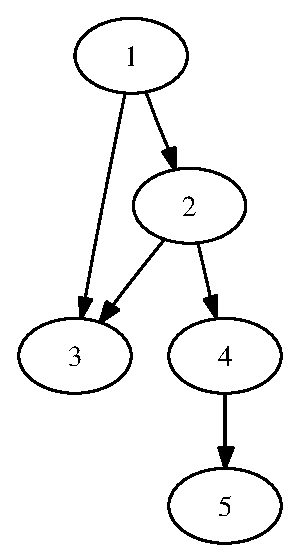
\epsfig{file=Figures/graph0,scale=0.6}

  \caption{A simple graph.}
  \label{fig:graph0}
\end{figure}



\noindent
The graph given by the relation \texttt{R} contains only the direct connections of vertices.  For example, in
the graph shown in Figure \ref{fig:graph0}, there is a direct connection from vertex $1$ to vertex $2$ and
another direct connection from vertex $2$ to vertex $4$.  Intuitively, vertex $4$ is reachable from vertex $1$,
since from vertex $1$ we can first reach vertex $2$ and from vertex $2$ we can then reach vertex $4$.  However,
there is is no direct connection between the vertices $1$ and $4$.  To make this more formal, define
a \colorbox{amethyst}{\blue{path}} 
of a graph $R$ as a list of vertices
\\[0.2cm]
\hspace*{1.3cm}
$[x_1, x_2, \cdots, x_n]$ \quad such that \quad $\pair(x_i,x_{i+1}) \in R$ \quad for all $i=1,\cdots,n-1$.
\\[0.2cm]
In this case, the path $[x_1, x_2, \cdots, x_n]$ is written as
\\[0.2cm]
\hspace*{1.3cm}
$x_1 \mapsto x_2 \mapsto \cdots \mapsto x_n$
\\[0.2cm]
and has the \blue{length} $n-1$.  It is important to note that the length of a path
$[x_1,x_2,\cdots,x_n]$ is defined as the number of edges connecting the vertices and not as the
number of vertices appearing in the path.

Furthermore,  two vertices $a$ and $b$ are said to be \colorbox{amethyst}{\blue{connected}} iff there exists a path
\\[0.2cm]
\hspace*{1.3cm}
$[x_1,\cdots,x_n]$ \quad such that \quad $a = x_1$ \quad and \quad $b = x_n$.
\\[0.2cm]
The goal of this section is to develop an algorithm that checks whether two vertices $a$ and $b$ are connected.
Furthermore, we want to be able to compute the corresponding path connecting the vertices $a$ and $b$.


\subsection{Computing the Transitive Closure of a Relation}
We have already noted that a graph can be represented as the set of its edges and hence as a \blue{relation}.
In order to decide whether there is a path connecting two vertices we have to compute the 
\href{https://en.wikipedia.org/wiki/Transitive_closure}{transitive closure} $R^+$ of a relation $R$.  
In the \href{https://github.com/karlstroetmann/Lineare-Algebra/blob/master/Script/lineare-algebra.pdf}{math lecture}
we have seen that the transitive closure $R^+$ can be computed as follows:
\\[0.2cm]
\hspace*{1.3cm}
$R^+ = \bigcup\limits_{n=1}^{\infty} R^n = R^1 \cup R^2 \cup R^3 \cup \cdots$  
\\[0.2cm]
Initially, this formula might look intimidating as it suggests an infinite computation.
Fortunately, it turns out that we do not have to compute all powers of the form $R^n$.  Let me
explain the reason that allows us to cut the computation short.  
\begin{enumerate}
\item $R$ is the set of direct connections between two vertices.
\item $R^2$ is the same as $R \circ R$ and this relational product is defined as
      \\[0.2cm]
      \hspace*{1.3cm}
       $R \circ R = \{ \pair(x,z) \mid \exists y \colon \pair(x,y) \in R \wedge \pair(y,z) \in R \}$.
      \\[0.2cm]
      Hence, $R \circ R$ contains those pairs $\pair(x,z)$ that are connected via one intermediate vertex $y$,
      i.e.~there is a path of the form $x \mapsto y \mapsto z$ that connects $x$ and $z$.  This path
      has length 2.  In general, we can show by induction that $R^n$ connect those pairs that are
      connected by a path of length $n$.  The induction step of this proof runs as follows:
\item $R^{n+1}$ is defined as $R \circ R^{n}$ and therefore we have
      \\[0.2cm]
      \hspace*{1.3cm}
      $R \circ R^n = \{ \pair(x,z) \mid \exists y \colon \pair(x,y) \in R \wedge \pair(y,z) \in R^n \}$.
      \\[0.2cm]
      As $\pair(y,z) \in R^n$, the induction hypothesis guarantees that the vertices $y$ and $z$ are
      connected by a path of length $n$.  Hence, this 
      path has the form
      \\[0.2cm]
      \hspace*{1.3cm}
      $\underbrace{y \mapsto \cdots \mapsto z}_{\mbox{\scriptsize path of length $n$.}}$
      \\[0.2cm]
      Adding $x$ at the front of this path will produce the path
      \\[0.2cm]
      \hspace*{1.3cm}
      $x \mapsto y \mapsto \cdots \mapsto z$.
      \\[0.2cm]
      This path has a length of $1 + n = n + 1$ and, furthermore, connects $x$ and $z$.  Hence $R^{n+1}$
      contains those pairs $\pair(x, z)$ that are connected by a path of length $n+1$.
\end{enumerate}
Now the important observation is the following. The set of all vertices is finite.  For the arguments sake, let
us assume there are $k$ vertices.  But then every path that has a length of  $k$ or greater must contain one
vertex that is visited at least twice and hence this path is longer than necessary, i.e.~there is a shorter path that
connects the same vertices.  Therefore, for a finite graph with $k$ vertices, the formula to compute the
transitive closure can be simplified as follows:
\\[0.2cm]
\hspace*{1.3cm} 
$\ds R^+ = \bigcup\limits_{i=1}^{k-1} R^i$.
\\[0.2cm]
While we could use this formula as its stands, it is more efficient to use a \blue{fixed-point iteration} instead.
To this end, we prove that the transitive closure $R^+$ satisfies the following equation:
\begin{equation}
  \label{fixpunkt}
  R^+ = R \cup R \circ R^+. 
\end{equation}
Let me remind you that the precedence of the operator $\circ$ 
is higher than the precedence of the operator $\cup$.  Therefore, the expression $R \cup R \circ R^+$ is parenthesized
as $R \cup (R \circ R^+)$.  Equation \ref{fixpunkt} can be proven algebraically.  We have:
\\[0.2cm]
\hspace*{1.3cm}
$
\begin{array}{cll}
    & R \cup R \circ R^+ \\[0.2cm]
  = & R \cup R \circ \bigcup\limits_{i=1}^{\infty} R^i \\[0.4cm]
  = & R \cup R \circ \bigl(R^1 \cup R^2 \cup R^3 \cup \cdots \bigr) \\[0.2cm]
  = & R \cup \bigl(R \circ R^1 \cup R \circ R^2 \cup R \circ R^3 \cup \cdots \bigr) \\[0.2cm]
  = & R \cup \bigl(R^2 \cup R^3 \cup  R^4 \cup \cdots \bigr)  \\[0.2cm]
  = & R^1 \cup \bigl(R^2 \cup R^3 \cup  R^4 \cup \cdots \bigr) \\[0.2cm]
  = & \bigcup\limits_{i=1}^{\infty} R^i \\[0.4cm]
  = & R^+.
\end{array}
$
\\[0.2cm]
Equation  \ref{fixpunkt} can now be used to compute $R^+$ via a fixed-point iteration.
To this end, let us define a sequence of relations $(T_n)_{n \in \mathbb{N}}$ by induction on $n$:
\begin{enumerate}
\item[I.A.] $n = 0$: 

            $T_0 = R$
\item[I.S.] $n \mapsto n+1$:

            $T_{n+1} = R \cup R \circ T_n$. 
\end{enumerate}
The relation  $T_n$ can be expressed via the relation $R$, we have
\begin{enumerate}
\item $T_0 = R$.
\item $T_1 = R \cup R \circ T_0 = R \cup R \circ R = R^1 \cup R^2$.
\item$\begin{array}[t]{lcl}
       T_2  & = & R \cup R \circ T_1 \\
            & = & R \cup R \circ (R^1 \cup R^2) \\
            & = & R^1 \cup R^2 \cup R^3. \\
       \end{array}
      $
\end{enumerate}
In general, we can show by induction that
\\[0.2cm]
\hspace*{1.3cm}
$T_n = \bigcup\limits_{i=1}^{n+1} R^i$
\\[0.2cm]
holds for all $n \in \mathbb{N}$.  The base case of this proof is immediate form the definition of $T_0$.
In the induction step we observe the following:
\\[0.2cm]
\hspace*{1.3cm}
$
 \begin{array}{lcll}
   T_{n+1} & = & \ds R \cup R \circ T_n & \mbox{(by definition)} \\[0.2cm]
           & = & \ds R \cup R \circ \biggl(\bigcup\limits_{i=1}^{n+1} R^i\biggr) &
                 \mbox{(by induction hypothesis)} \\[0.4cm]
           & = & \ds R \cup R \circ \left(R \cup \cdots \cup R^{n+1}\right) \\[0.2cm] 
           & = & \ds R \cup R^2 \cup \cdots \cup R^{n+2}  &
                 \mbox{(by the distributivity of $\circ$ over $\cup$)} \\[0.2cm]
           & = & \ds \bigcup\limits_{i=1}^{n+2} R^i & \Box 
   \end{array}
$
\\[0.2cm]
The sequence $(T_n)_{n\in\mathbb{N}}$ has another useful property:  It is 
\blue{monotonically increasing}.  In general, a sequence of sets $(X_n)_{n\in\mathbb{N}}$ is called
\blue{monotonically increasing} iff we have
\\[0.2cm]
\hspace*{1.3cm}
$\forall n \in \mathbb{N}: X_n \subseteq X_{n+1}$,
\\[0.2cm]
i.e.~the sets $X_n$ get bigger with growing index $n$.
The monotonicity of the sequence  $(T_n)_{n \in \mathbb{N}}$ is an immediate consequence of the equation
\\[0.2cm]
\hspace*{1.3cm}
$\ds T_n = \bigcup\limits_{i=1}^{n+1} R^i$ 
\\[0.2cm]
because we have:
\\[0.2cm]
\hspace*{1.3cm}
$
\begin{array}[t]{llcl}
                & \ds T_n \subseteq T_{n+1} \\[0.2cm]
\Leftrightarrow & \ds \bigcup\limits_{i=1}^{n+1} R^i \subseteq \bigcup\limits_{i=1}^{n+2} R^i \\[0.5cm]
\Leftrightarrow & \ds \bigcup\limits_{i=1}^{n+1} R^i \subseteq \bigcup\limits_{i=1}^{n+1} R^i \cup R^{n+2} \\
\end{array}
$
\\[0.2cm]
If the relation  $R$ is finite, then the transitive closure $R^+$ is finite, too.  The sets $T_n$ 
are all subsets of $R^+$ because we have
\\[0.2cm]
\hspace*{1.3cm}
$\ds T_n = \bigcup\limits_{i=1}^{n+1} R^i \subseteq \bigcup\limits_{i=1}^{\infty} R^i = R^+$ \quad for all $n \in \mathbb{N}$.
\\[0.2cm]
Hence the sets $T_n$ can not grow indefinitely.  Because of the monotonicity of the sequence 
$(T_n)_{n\in\mathbb{N}}$ it follows that there exists an index  $k \in \mathbb{N}$ such that the sets $T_n$ do
not grow any further once $n$ has reached $k$, i.e.~we have
\\[0.2cm]
\hspace*{1.3cm}
$\ds \forall n \in \mathbb{N}:( n \geq k \rightarrow T_n = T_k)$.
\\[0.2cm]
But this implies that
\\[0.2cm]
\hspace*{1.3cm}
$\ds T_n = \bigcup\limits_{i=1}^{n+1} R^i = \bigcup\limits_{i=1}^{\infty} R^i = R^+$ 
\quad holds for all $n \geq k$.
\\[0.2cm]
Therefore, the algorithm for computing  $R^+$ iterates the equation 
\\[0.2cm]
\hspace*{1.3cm}
$\ds T_{n+1} = R \cup R \circ T_n$
\\[0.2cm]
until the equation  $T_{n+1} = T_n$ is satisfied, since this implies that $T_n = R^+$.


\begin{figure}[!ht]
  \centering
\begin{Verbatim}[ frame         = lines, 
                  framesep      = 0.3cm, 
                  labelposition = bottomline,
                  numbers       = left,
                  numbersep     = -0.2cm,
                  xleftmargin   = 0.8cm,
                  xrightmargin  = 0.8cm,
                ]
    transClosure = procedure(R) {
        T = R;
        while (true) {
            oldT = T;
            T    = R + product(R, T);
            if (T == oldT) {
                return T;
            }
        }
    };
    product = procedure(R1, R2) {
        return { [x,z] : [x,y] in R1, [y,z] in R2 };
    };
    R = { [1,2], [2,3], [1,3], [2,4], [4,5] };
    print( "R = ", R );
    print( "Computing the transitive closure of R:" );
    T = transClosure(R);
    print( "R+ = ", T );
\end{Verbatim} 
\vspace*{-0.3cm}
\caption{Computing the transitive closure.}  
\label{fig:transitive-closure.py}
\end{figure} %\$

\noindent
The program 
\href{https://github.com/karlstroetmann/Logik/blob/master/Python/transitive-closure.py}{\texttt{transitive-closure.py}}
that is shown in Figure
\ref{fig:transitive-closure.py} on page \pageref{fig:transitive-closure.py} shows an implementation of this idea.
The program produces the following output:
\begin{verbatim}
    R = {[1, 2], [2, 3], [1, 3], [2, 4], [4, 5]}
    Computing the transitive closure of R:
    R+ = {[1, 2], [1, 3], [1, 4], [1, 5], [2, 3], [2, 4], [2, 5], [4, 5]}
\end{verbatim}
The transitive closure $R^+$ of a relation $R$ has a very intuitive interpretation:
$R^+$:  It contains all pairs $\pair(x,y)$ such that there is a path leading from 
$x$ to $y$.  
The function $\texttt{product}(R_1, R_2)$ computes the relational product $R_1\circ R_2$ 
according to the formula
\\[0.2cm]
\hspace*{1.3cm}
$R_1 \circ R_2 = \{ \langle x, z \rangle \mid \exists y: \pair(x,y) \in R_1 \wedge \pair(y,z) \in R_2 \}$.
\\[0.2cm]
The implementation of the procedure \texttt{product} shows the most general way to define a set in
\textsl{Python}.  In general, a set can be defined via an expression of the form
\\[0.2cm]
\hspace*{1.3cm}
$\{\; \textsl{expr} \;\texttt{:}\; [x^{(1)}_1, \cdots, x^{(1)}_{n(1)}] \;\texttt{in}\; s_1,
     \cdots, [x^{(k)}_1, \cdots, x^{(k)}_{n(k)}] \;\texttt{in}\; s_k \;\texttt{|}\;
     \textsl{cond} \;\}
$.
\\[0.2cm]
Here, for all $i=1, \cdots, k$ the variable $s_i$ denotes a set of lists of length $n(i)$.  When the
expression given above is evaluated, the variables $x^{(i)}_1, \cdots, x^{(i)}_{n(i)}$ are replaced
by the corresponding values in the lists from the sets  $s_i$.  For example, if we define
\begin{verbatim}
    s1 = { [ 1, 2, 3 ], [ 5, 6, 7 ] };
    s2 = { [ "a", "b" ], [ "c", "d" ] };
    m = { [ x1, x2, x3, y1, y2 ] : [ x1, x2, x3 ] in s1, [ y1, y2 ] in s2 };
\end{verbatim}
then the set  \texttt{m} has the following value:
\begin{verbatim}
    { [1, 2, 3, "a", "b"], [5, 6, 7, "c", "d"],  
      [1, 2, 3, "c", "d"], [5, 6, 7, "a", "b"] }
\end{verbatim}


\subsection{Computing the Paths}
So far, given a graph represented by a relation $R$ and two vertices $x$ and $y$, we can only check
whether there is a path leading from $x$ to $y$, but we cannot compute this path.  In this
subsection we will extend the procedure \texttt{transClosure} so that it will also compute the
corresponding path.  The main idea is to extend the notion of a relational product to the notion of
a \blue{path product}, where a \blue{path product} is defined on sets of paths.  In order to do so,
we introduce three functions for lists.
\begin{enumerate}
\item Given a list $p$, the function $\texttt{first}(p)$ returns the first element of $p$: 
      \\[0.2cm]
      \hspace*{1.3cm}
      $\texttt{first}\bigl([x_1,\cdots,x_m]\bigr) = x_1$.
\item Given a list $p$, the function $\texttt{last}(p)$ returns the last element of $p$: 
      \\[0.2cm]
      \hspace*{1.3cm}
      $\texttt{last}\bigl([x_1,\cdots,x_m]\bigl) = x_m$.
\item If $p = [ x_1, \cdots, x_m ]$ and $q =[ y_1, \cdots, y_n ]$ are two path such that
      $\texttt{first}(q) = \texttt{last}(p)$, we define the \blue{join} of $p$ and $q$ as \\[0.2cm]
      \hspace*{1.3cm}
      $p \oplus q = [x_1, \cdots, x_m, y_2, \cdots, y_n ]$.
\end{enumerate}
If $P_1$ and $P_2$ are sets of paths, we define the  \blue{path product} of
$P_1$ and $P_2$ as follows: \\[0.2cm]
\hspace*{1.3cm} 
$P_1 \bullet P_2 = 
\bigl\{\; p_1 \oplus p_2 \mid p_1 \in P_1 \wedge p_2 \in P_2 \wedge \texttt{last}(p_1) =
\texttt{first}(p_2) \;\bigr\}
$.

\begin{figure}[!ht]
  \centering
\begin{Verbatim}[ frame         = lines, 
                  framesep      = 0.3cm, 
                  labelposition = bottomline,
                  numbers       = left,
                  numbersep     = -0.2cm,
                  xleftmargin   = 0.8cm,
                  xrightmargin  = 0.8cm,
                ]
    transClosure = procedure(R) {
        P = R;
        while (true) {
            oldP = P;
            P    = R + pathProduct(R, P);
            print(P);
            if (P == oldP) {
                return P;
            }
        }
    };
    pathProduct = procedure(P, Q) {
        return { join(x, y) : x in P, y in Q | x[-1] == y[1] };
    };    
    join = procedure(p, q) {
        return p + q[2..];
    };
    R = { [1,2], [2,3], [1,3], [2,4], [4,5] };
    print( "R = ", R );
    print( "computing all paths" );
    P = transClosure(R);
    print( "P = ", P );
\end{Verbatim} 
\vspace*{-0.3cm}
\caption{Computing all connections.}  \label{fig:path.py}
\end{figure} %\$

\begin{figure}[!ht]
  \centering
  \vspace*{-9cm}

  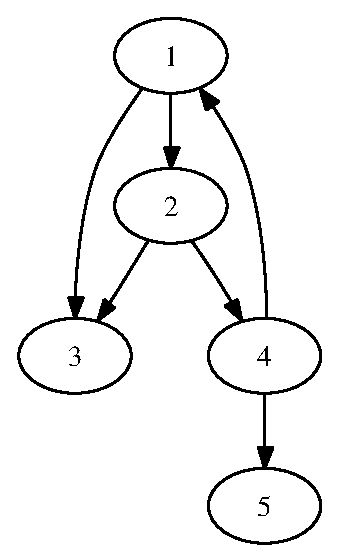
\epsfig{file=Figures/graph-zykl,scale=0.5}
  \vspace*{-1cm}

  \caption{A graph with a cycle.}
  \label{fig:graph-zykl}
\end{figure}

Using the notion of a \blue{path product} we are able to extend the program shown in Figure
\ref{fig:transitive-closure.py} such that it computes all paths between two vertices.
The resulting program
\href{https://github.com/karlstroetmann/Logik/blob/master/Python/path.py}{\texttt{path.py}}
is shown in Figure \ref{fig:path.py} on page \pageref{fig:path.py}.
Unfortunately, the program does not work any more if the graph is \blue{cyclic}.  A graph is defined
to be \blue{cyclic} if there is a path of length greater than $1$ that starts and ends at the same
vertex.  This path is then called a \blue{cycle}.
Figure \ref{fig:graph-zykl} on page \pageref{fig:graph-zykl} shows a cyclic graph.  This graph is
cyclic because it contains the path
\\[0.2cm]
\hspace*{1.3cm}
\texttt{[1, 2, 4, 1]}
\\[0.2cm]
and this path is a cycle.
The problem with this graph is that it contains an infinite number of paths that connect the vertex
1 with the vertex 2: \\[0.2cm]
\hspace*{1.3cm}
$[ 1, 2 ]$, $[ 1, 2, 4, 1, 2 ]$, 
$[ 1, 2, 4, 1, 2, 4, 1, 2 ]$, 
$[ 1, 2, 4, 1, 2, 4, 1, 2, 4, 1, 4 ]$, $\cdots$
\\[0.2cm]
Of course, there is no point in computing a path that visits a vertex more than once as these paths
contain cycles.  Our goal is to eliminate all those paths that contain cycles.


\begin{figure}[!ht]
  \centering
\begin{Verbatim}[ numbers       = left,
                  numbersep     = -0.2cm,
                  frame         = lines, 
                  framesep      = 0.3cm, 
                  labelposition = bottomline,
                  xleftmargin   = 0.0cm,
                  xrightmargin  = 0.0cm,
                ]
    pathProduct = procedure(P, Q) {
        return { join(x,y) : x in P, y in Q | x[-1] == y[1] && noCycle(x, y) };
    };
    noCycle = procedure(L1, L2) {
        return #({ x : x in L1 } * { x : x in L2 }) == 1;
    };
\end{Verbatim} 
\vspace*{-0.3cm}
\caption{Computing the connections in a cyclic graph.}  
\label{fig:path-cyclic.py}
\end{figure} %\$

Figure \ref{fig:path-cyclic.py} on page shows how the implementation of the function
\texttt{pathProduct} has to be changed so that the resulting program
\href{https://github.com/karlstroetmann/Logik/blob/master/Python/path-cyclic.py}{\texttt{path-cyclic.py}}
works also for cyclic graphs. 
\begin{enumerate}
\item In line 2, we compute only those paths that are not cyclic.
\item Line 5 tests, whether the join  $\texttt{L1} \oplus \texttt{L2}$ is cyclic.  The join
      of \texttt{L1} and \texttt{L2} is cyclic iff the lists \texttt{L1} and \texttt{L2} have more
      than one common element. 
      The lists \texttt{L1} and \texttt{L2} will always have at least one common element, as we join
      these lists only if the last element of \texttt{L1} is equal to the first element of  \texttt{L2}.
      If there would be an another vertex common to \texttt{L1} and \texttt{L2}, then the path
      $\texttt{L1} \oplus \texttt{L2}$ would be cyclic.
\end{enumerate}

In general, we are not really interested to compute all possible paths between two given vertices
\texttt{x} and \texttt{y}.  Instead, we just want to compute the shortest path leading from \texttt{x} to \texttt{y}.
Figure \ref{fig:find-path.py} on page \pageref{fig:find-path.py} shows the procedure \texttt{reachable}. 
This procedure takes three arguments:
\begin{enumerate}
\item \texttt{x} and \texttt{y} are vertices of a graph.
\item \texttt{R} is a binary relation representing a directed graph.
\end{enumerate}
The call  \texttt{reachable(x, y, R)} checks whether \texttt{x} and \texttt{y} are connected and, furthermore,
computes the shortest path from \texttt{x} to \texttt{y}, provided such a path exists.
The complete program can be found in the file
\href{https://github.com/karlstroetmann/Logik/blob/master/Python/find-path.py}{\texttt{find-path.py}}.
Next, we discuss the implementation of the procedure  \texttt{reachable}.
\begin{enumerate}
\item Line 2 initializes the set \texttt{P}.  After $n$ iterations, this set will contain all paths
      that start in the vertex \texttt{x} and that have a length of at most $n$.

      Initially, there is just the trivial path \texttt{[x]} that starts in \texttt{x} and has
      length $0$.
\item Line 5 tries to extend all previously computed paths by one step.
      If we are lucky, the set \texttt{P} is increased in this step.
\item Line 6 selects all those paths from the set \texttt{P} that lead to the vertex \texttt{y}.
      These paths are stored in the set \texttt{Found}.
\item Line 7 checks whether we have indeed found a path ending at \texttt{y}.  This is the case if
      the set \texttt{Found} is not empty.  
      In this case, we return any of these paths.
\item If we have not yet found the vertex \texttt{y} and, furthermore, we have not been able to find
      any new paths during this iteration,  the procedure returns in line 11.
      As the \texttt{return} statement in line 11 does not return a value, the procedure will
      instead return the undefined value $\Omega$.
\end{enumerate}
The procedure call \texttt{reachable(x,y R)} will compute the \textbf{shortest} path connecting
\texttt{x} and \texttt{y} because it computes path with increasing length.  The first iteration
computes all paths starting in \texttt{x} that have a length of at most 1, the second iteration
computes all paths starting in \texttt{x} that have a length of at most 2, and in general the $n$-th
iteration computes all paths starting in \texttt{x} that have a length of at most $n$.  Hence, if
there is a path of length $n$, then this path will be found in the $n$-iteration unless a shorter path has
already been found in a previous iteration.  

\remarkEng
The algorithm described above is known as 
\href{https://en.wikipedia.org/wiki/Breadth-first_search}{breadth first search}. \eox 



\begin{figure}[!ht]
  \centering
\begin{Verbatim}[ frame         = lines, 
                  framesep      = 0.3cm, 
                  labelposition = bottomline,
                  numbers       = left,
                  numbersep     = -0.2cm,
                  xleftmargin   = 0.8cm,
                  xrightmargin  = 0.8cm,
                ]
    reachable = procedure(x, y, R) {
        P = { [x] };
        while (true) {
            oldP  = P;
            P     = P + pathProduct(P, R);
            Found = { l : l in P | l[-1] == y };
            if (Found != {}) {
                return arb(Found);
            }
            if (P == oldP) {
                return;
            }
        }
    };
\end{Verbatim} 
\vspace*{-0.3cm}
\caption{Finding the shortest path between two vertices.}  
\label{fig:find-path.py}
\end{figure}

\subsection{The Wolf, the Goat, and the Cabbage}
Next, we present an application of the theory developed so far.  We solve a problem from that has puzzled
the greatest agricultural economists for centuries.  The puzzle we want to solve is known as the 
\href{http://jeux.lulu.pagesperso-orange.fr/html/anglais/loupChe/loupChe1.htm}{wolf-goat-cabbage puzzle}:  
\vspace*{0.3cm}

\begin{minipage}[c]{14cm}
{\sl
An agricultural economist has to sell a wolf, a goat, and a cabbage on a market place.  In order to
reach the market place, she has to cross a river.  The boat that she can use is so small that it can
only accommodate either the goat, the wolf, or the cabbage in addition to the agricultural economist.
Now if the agricultural economist leaves the wolf alone with the goat, the wolf will eat the goat.
If, instead, the agricultural economist leaves the goat with the cabbage, the goat will eat the cabbage.
Is it possible for the agricultural economist to develop a schedule that allows her to cross the river
without either the goat or the cabbage being eaten?
}
\end{minipage}
\vspace*{0.3cm}

\noindent
In order to compute a schedule, we first have to model the problem.  The various \blue{states} of the problem will
be regarded as \blue{vertices} of a graph and this graph will be represented as a binary relation.
To this end we define the set
\\[0.2cm]
\hspace*{1.3cm} 
$\texttt{All} = \{ \squote{farmer}, \squote{wolf}, \squote{goat},\squote{cabbage} \}$.
\\[0.2cm]
Every node will be represented as a subset \texttt{S} of the set \texttt{All}.  The idea is that the set \texttt{S}
specifies those objects that are on the left side of the river.  We assume that initially the farmer
is on the left side of the river. 
Therefore, the set of all possible states can be defined as the set
\begin{verbatim}
        P = { S : S in 2 ** All | !problem(S) && !problem(All - S) };
\end{verbatim}
Here, we have used the procedure \texttt{problem} to check whether a given set \texttt{S} has a problem. 
Note that since \texttt{S} is the set of objects on the left side, the expression $\texttt{All - S}$
computes the set of objects on the right side of the river.

Next, a set \texttt{S} of objects has a problem if both of the following conditions
are satisfied:
\begin{enumerate}
\item The farmer is not an element of \texttt{S} and
\item either \texttt{S} contains both the goat and the cabbage or \texttt{S} contains both the wolf and the goat.
\end{enumerate}
Therefore, we can implement the function \texttt{problem} as follows:

\begin{verbatim}
    problem = procedure(S) {
        return !("farmer" in S)                                     && 
               ({"goat", "cabbage"} <= S || {"wolf", "goat"} <= S);
    };
\end{verbatim}
We proceed to compute the relation \texttt{R} that contains all possible transitions between
different states.  We will compute \texttt{R} using the formula:
\\[0.2cm]
\hspace*{0.75cm}
\texttt{R = R1 + R2;}
\\[0.2cm]
Here \texttt{R1} describes the transitions that result from the farmer crossing the river from left
to right, while \texttt{R2} describes the transitions that result from the farmer crossing the river
from right to left.  We can define the relation \texttt{R1} as follows:
\begin{verbatim}
    R1  = { [S, S - B]: S in P, B in 2 ** S
                       | S - B in P && "farmer" in B && #B <= 2
           };
\end{verbatim}
Let us explain this definition in detail:
\begin{enumerate}
\item Initially, \texttt{S} is the set of objects on the left side of the river.  Hence, \texttt{S}
      is an element of the set of all states that we have defined as \texttt{P}.
\item \texttt{B} is the set of objects that are put into the boat and that do cross the river.  Of
      course, for an object to go into the boat is has to be on the left side of the river to begin
      with.  Therefore, \texttt{B} is a subset of \texttt{S} and hence an element of the power set
      of \texttt{S}. 
\item Then  \texttt{S-B} is the set of objects that are left on the left side of the river after
      the boat has crossed.  Of course, the new state \texttt{S-B} has to be a state that does not
      have a problem.  Therefore, we check that \texttt{S-B} is an element of \texttt{P}.
\item Furthermore, the farmer has to be in the boat.  This explains the condition 
      \\[0.2cm]
      \hspace*{1.3cm}
      \texttt{\symbol{39}farmer\symbol{39} in B}.
\item Finally, the boat can only have two passengers.  Therefore, we have added the condition
      \\[0.2cm]
      \hspace*{1.3cm}
      \texttt{\#B <= 2}.
\end{enumerate}
Next, we have to define the relation \texttt{R2}.  However, as crossing the river from right to left
is just the reverse of crossing the river from left to right, \texttt{R2} is just the inverse of
\texttt{R1}.   Hence we define:
\\[0.2cm]
\hspace*{1.3cm}
\texttt{R2  = \{ [y, x] : [x, y] in R1 \};}
\\[0.2cm]
Finally, the start state has all objects on the left side.  Therefore, we have
\\[0.2cm]
\hspace*{1.3cm}
\texttt{start = All;}
\\[0.2cm]
In the end, all objects have to be on the right side of the river.  That means that nothing is left
on the left side.  Therefore, we define
\\[0.2cm]
\hspace*{1.3cm}
\texttt{goal = \{\};}
\\[0.2cm]
Figure \ref{fig:wolf-ziege} on page \pageref{fig:wolf-ziege} shows the program
\href{https://github.com/karlstroetmann/Logik/blob/master/Python/wolf-goat-cabbage.py}{\texttt{wolf-goat-cabbage.py}}
that combines the statements shown so far.  The solution computed by this program is shown in Figure
 \ref{fig:wolf-ziege-solution}.

\begin{figure}[!ht]
  \centering
\begin{Verbatim}[ codes         = {\catcode`$=3\catcode`_=8\catcode`^=7},
                  frame         = lines, 
                  framesep      = 0.3cm, 
                  labelposition = bottomline,
                  numbers       = left,
                  numbersep     = -0.2cm,
                  xleftmargin   = 0.8cm,
                  xrightmargin  = 0.8cm,
                ]
    problem = procedure(S) {
        return !("farmer" in S)                                     && 
               ({"goat", "cabbage"} <= S || {"wolf", "goat"} <= S);
    };
    
    All = { "farmer", "wolf", "goat", "cabbage" };
    P   = { S : S in 2 ** All | !problem(S) && !problem(All - S) };
    R1  = { [S, S - B]: S in P, B in 2 ** S
                       | S - B in P && "farmer" in B && #B <= 2
           };
    R2  = { [y, x] : [x, y] in R1 };
    R   = R1 + R2;
    
    start = All;
    goal  = {};
    
    path  = reachable(start, goal, R);
\end{Verbatim} 
\vspace*{-0.3cm}
\caption{Solving the wolf-goat-cabbage problem.}  
\label{fig:wolf-ziege}
\end{figure}


\begin{figure}[!ht]
  \centering
\begin{Verbatim}[ codes         = {\catcode`$=3\catcode`_=8\catcode`^=7},
                  frame         = lines, 
                  framesep      = 0.3cm, 
                  labelposition = bottomline,
                  numbers       = left,
                  numbersep     = -0.2cm,
                  xleftmargin   = 0.8cm,
                  xrightmargin  = 0.8cm,
                ]
    {"cabbage", "farmer", "goat", "wolf"}                                 {}
                             >>>> {"farmer", "goat"} >>>> 
    {"cabbage", "wolf"}                                   {"farmer", "goat"}
                             <<<< {"farmer"} <<<< 
    {"cabbage", "farmer", "wolf"}                                   {"goat"}
                             >>>> {"farmer", "wolf"} >>>> 
    {"cabbage"}                                   {"farmer", "goat", "wolf"}
                             <<<< {"farmer", "goat"} <<<< 
    {"cabbage", "farmer", "goat"}                                   {"wolf"}
                             >>>> {"cabbage", "farmer"} >>>> 
    {"goat"}                                   {"cabbage", "farmer", "wolf"}
                             <<<< {"farmer"} <<<< 
    {"farmer", "goat"}                                   {"cabbage", "wolf"}
                             >>>> {"farmer", "goat"} >>>> 
    {}                                 {"cabbage", "farmer", "goat", "wolf"}
\end{Verbatim} 
\vspace*{-0.3cm}
\caption{A schedule for the agricultural economist.}  
\label{fig:wolf-ziege-solution}
\end{figure}


\section{Terms and Matching}
So far we have seen the basic data structures of \setlx\ like numbers, string, sets, and lists.
There is one more data structure that is supported by \setlx.  This is the data structure of
\colorbox{amethyst}{\blue{terms}}.  
This data structure is especially useful when we develop programs that deal with mathematical formulas.
For example, in this section we will develop a program that reads a string like 
\\[0.2cm]
\hspace*{1.3cm}
``\texttt{x * exp(x)}'',
\\[0.2cm]
interprets this string as describing the real valued function 
\\[0.2cm]
\hspace*{1.3cm}
$x \mapsto x \cdot \exp(x)$, 
\\[0.2cm]
and then takes the derivative of this function with respect to the variable $x$.  This program is
easy to implement if real valued functions are represented as terms.  The reason is that \setlx\ provides 
\colorbox{amethyst}{\blue{matching}} for terms.  We will define this notion later.  Matching
is one of the main ingredients of the programming language \href{https://en.wikipedia.org/wiki/Prolog}{Prolog}.
This programming language was quite popular in artificial intelligence during the eighties and has
inspired the matching that is available in \textsl{Python}.


\subsection{Constructing and Manipulating Terms}
In order to build terms, we first need \colorbox{amethyst}{\blue{functors}}.  It is important not to confuse functors with
function symbols.  Therefore, functors have to be preceded by the character  
``\texttt{@}''.
For example, the following strings can be used as functors:
\\[0.2cm]
\hspace*{1.3cm}
\texttt{@f}, \quad \texttt{@FabcXYZ}, \quad \texttt{@sum}, \quad \texttt{@Hugo\_}.
\\[0.2cm]
However, in the expression ``\texttt{@f}'', the string ``\texttt{f}'' is the functor.  The
character ``\texttt{@}'' is only used as an escape character that tells us that ``\texttt{f}'' is
not a function symbol but rather a functor.  Next, we define \colorbox{amethyst}{\blue{terms}}.  If $F$ is a functor and 
$t_1$, $t_2$, $\cdots$, are any values, i.e.~they could be number, strings, lists, sets, or terms
themselves, then
\\[0.2cm]
\hspace*{1.3cm}
$\texttt{@}F(t_1, t_2, \cdots, t_n)$
\\[0.2cm]
is a term.  Syntactically, terms look very similar to function calls.  The only difference between a function call
and a term is the following: 
\begin{enumerate}
\item A function call starts with a function symbol. 
\item A term starts with a functor. 
\end{enumerate}


\examplesEng
\begin{enumerate}
\item \texttt{@Address(\symbol{39}Coblitzallee 1-9\symbol{39}, 68163, \symbol{39}Mannheim\symbol{39})}

      is a term that represents an address.
\item \texttt{@product(@variable(\symbol{39}x\symbol{39}), @exp(@variable(\symbol{39}x\symbol{39})))}

      is a term that represents the  function $x \mapsto x \cdot \exp(x)$.  
      \eox
\end{enumerate}
At this point you might ask how terms are evaluated.  The answer is that terms
\colorbox{amethyst}{are not evaluated!}  
Terms are used to represent data in a way that is both concise and readable.  Hence, terms are values like
numbers, sets or strings.  As terms are values, they don't need to be evaluated.

Let us demonstrate a very simple application of terms.  Imagine that \setlx\ wouldn't provide lists as a native data
type.  Then, we could implement lists via terms.  First, we would use a functor to represent the empty list.
Let us choose the functor \texttt{nil} for this purpose.  Hence, we have
\\[0.2cm]
\hspace*{1.3cm}
$\texttt{@nil()} \;\widehat{=}\; \texttt{[]}$,
\\[0.2cm]
where we read the symbol ``$\widehat{=}$'' as ``corresponds to''.
Note that the parentheses after the functor  \texttt{nil} are \colorbox{amethyst}{necessary!}  Next, in order to represent
a list with first element $x$ and a list $r$ of remaining elements we use the functor \texttt{cons}.
Then we have the correspondence
\\[0.2cm]
\hspace*{1.3cm}
$\texttt{@cons}(x, r) \;\widehat{=}\; \texttt{[}x\texttt{]} + r$. 
\\[0.2cm]
Concretely, the list \texttt{[1,2,3]} is represented as the term
\\[0.2cm]
\hspace*{1.3cm}
\texttt{@cons(1, @cons(2, @cons(3, @nil())))}.
\\[0.2cm]
The programming language \textsl{Prolog} represents lists internally in a similar form.

\setlx\ provides two functions that allow us to extract the components of a term.  Furthermore, there is a
function for constructing terms.  These functions are described next.
\begin{enumerate}
\item The function \texttt{fct} returns the functor of a given term.
      If  $t$ is a term of the form $\at F(s_1,\cdots,s_n)$, then the result returned by the expression
      \\[0.2cm]
      \hspace*{1.3cm}
      $\texttt{fct}(\at F(s_1,\cdots,s_n))$
      \\[0.2cm]
      is the functor $F$ of this term.  For example the expression
      \\[0.2cm]
      \hspace*{1.3cm}
      \texttt{fct(@cons(1, @cons(2, @cons(3, @nil()))))}
      \\[0.2cm]
      returns the string  \texttt{\symbol{39}cons\symbol{39}} as its result.
\item The function \texttt{args} returns the arguments of a term.
      If  $t$ is a term of the form $\at F(s_1,\cdots,s_n)$, then
      \\[0.2cm]
      \hspace*{1.3cm}
      $\mathtt{args}(\at F(s_1,\cdots,s_n))$
      \\[0.2cm]
      returns the list $[s_1, \cdots, s_n]$. For example, the expression
      \\[0.2cm]
      \hspace*{1.3cm}
      \texttt{args(\at cons(1, \at cons(2, \at cons(3, \at nil()))))}
      \\[0.2cm]
      is evaluated as
      \\[0.2cm]
      \hspace*{1.3cm}
      \texttt{[1, \at cons(2, \at cons(3, \at nil()))]}.
\item If $f$ is the name of a functor and  $l$ is a list, then the function \texttt{makeTerm} can be invoked as
      \\[0.2cm]
      \hspace*{1.3cm}
      $t \;\mathtt{=}\; \texttt{makeTerm}(f,l)$.
      \\[0.2cm]
      This expression generates a term $t$ such that $f$ is the functor and $l$ is the list of its
      arguments.  Therefore we have
      \\[0.2cm]
      \hspace*{1.3cm}
      $\mathtt{fct}(t) = f$  \quad und \quad $\mathtt{args}(t) = l$.
      \\[0.2cm]
      For example, the expression
      \\[0.2cm]
      \hspace*{1.3cm}
      \texttt{makeTerm(\symbol{39}cons\symbol{39}, [ 1, \at nil() ])}
      \\[0.2cm]
      returns the result
      \\[0.2cm]
      \hspace*{1.3cm}
      \texttt{\at cons(1, \at nil())}.
\end{enumerate}

\begin{figure}[!ht]
\centering
\begin{Verbatim}[ frame         = lines, 
                  framesep      = 0.3cm, 
                  firstnumber   = 1,
                  labelposition = bottomline,
                  numbers       = left,
                  numbersep     = -0.2cm,
                  xleftmargin   = 0.8cm,
                  xrightmargin  = 0.8cm,
                ]
    append = procedure(l, x) {
        if (fct(l) == "nil") {
            return @cons(x, @nil());  
        }
        [head, tail] = args(l);
        return @cons(head, append(tail, x));
    };
    l = @cons(1, @cons(2, @cons(3, @nil()))); // corresponds to [1,2,3]
    print(append(l, 4));
\end{Verbatim}
\vspace*{-0.3cm}
\caption{Appending an element at the end of a list.}
\label{fig:append.py}
\end{figure}

Figure \ref{fig:append.py} on page \pageref{fig:append.py} shows the
program \href{https://github.com/karlstroetmann/Logik/blob/master/Python/append.py}{\texttt{append.py}}.
This program implements the function \texttt{append}.  As its first arguments, this function takes a list \texttt{l}
that is represented as a term.  As its second argument,  it takes an object \texttt{x}.  The purpose of the expression
\\[0.2cm]
\hspace*{1.3cm}
$\texttt{append}(\texttt{l}, \texttt{x})$
\\[0.2cm]
is to append the object \texttt{x} at the end of the list \texttt{l}.  The implementation of the function \texttt{append}
assumes that the list \texttt{l} is represented as a term using the functors ``\texttt{cons}'' and ``\texttt{nil}''.
\begin{enumerate}
\item Line 2 checks whether the list  \texttt{l} is empty. The list \texttt{l} is empty iff we have
      $\texttt{l} = \texttt{\at nil()}$.  In the program we merely check the functor of the term \texttt{l}.  If the name of this functor is
      \texttt{\symbol{39}nil\symbol{39}}, then \texttt{l} is the empty list.
\item If \texttt{l} is not empty, then it must be a term of the form
      \\[0.2cm]
      \hspace*{1.3cm}
      $\texttt{l} = \texttt{\at cons(\textsl{head}, \textsl{tail})}$.
      \\[0.2cm]     
      Then, conceptually \texttt{head} is the first element of the list \texttt{l} and \texttt{tail} is the list of
      the remaining elements.  In this case, we need to recursively append \texttt{t} at the end of the list \texttt{tail}.
      Finally, the first element of the list \texttt{l}, which is called \texttt{head} in line 5, needs
      to be prepended to the list that is returned from the recursive invocation of \texttt{append}.
      This is done in line 6 by constructing the term 
      \\[0.2cm]
      \hspace*{1.3cm}
      \texttt{@cons(head, append(tail, x))}.
\end{enumerate}

\subsection{Matching}
It would be quite tedious if the functions \texttt{fct} and \texttt{args} were the only means to extract the
components of a term.  Figure \ref{fig:append-match.py} on page \pageref{fig:append-match.py}
shows the program
\href{https://github.com/karlstroetmann/Logik/blob/master/Python/append-match.py}{\texttt{append-match.py}}, 
that uses \blue{matching} to implement the function \texttt{append}.  
Line 3 checks, whether the list  \texttt{l} is empty, i.e.~whether \texttt{l} is identical to the term 
\texttt{@nil()}.  Line 4 is more interesting, as it combines two actions.
\begin{enumerate}
\item It checks, whether the list \texttt{l} is a term that starts with the functor \texttt{cons}.
\item If \texttt{l} does indeed starts with the functor \texttt{cons}, the arguments of this functor are
      extracted and assigned to the variables \texttt{head} and \texttt{tail}.
\end{enumerate}
Hence, if the \texttt{match} statement in line 4 is successful, the equation
\\[0.2cm]
\hspace*{1.3cm}
$\texttt{l} = \texttt{@cons(head, tail)}$
\\[0.2cm]
holds afterwards.


\begin{figure}[!ht]
\centering
\begin{Verbatim}[ frame         = lines, 
                  framesep      = 0.3cm, 
                  firstnumber   = 1,
                  labelposition = bottomline,
                  numbers       = left,
                  numbersep     = -0.2cm,
                  xleftmargin   = 0.8cm,
                  xrightmargin  = 0.8cm,
                ]
    append = procedure(l, x) {
        match (l) {
            case @nil():            return @cons(x, @nil());
            case @cons(head, tail): return @cons(head, append(tail, x));
        }
    };
\end{Verbatim}
\vspace*{-0.3cm}
\caption{Implementing \texttt{append} using a \texttt{match} statement.}
\label{fig:append-match.py}
\end{figure}
In general, a \texttt{match} statement has the structure that is shown in Figure \ref{fig:match}.
Here, $e$ is any expression that yields a term when evaluated.  The expressions 
$t_1$, $\cdots$, $t_n$ are so called \blue{patterns} that contain variables.  When the \texttt{match} statement
is executed, \textsl{Python} tries to bind the variables occurring in the pattern $t_1$ such that the resulting
expression is equal to $e$.  If this succeeds, the statements in  $\textsl{body}_1$ are executed and the
execution of the \texttt{match} statement ends.
Otherwise, the patterns $t_2$, $\cdots$, $t_n$ are tried one by one.  If the pattern $t_i$ is successfully
matched to $e$, the statements in $\textsl{body}_i$ are executed and the execution of the \texttt{match}
statement end.  If none of the patterns $t_1$, $\cdots$, $t_n$ can be matched with $e$, the statements in
$\textsl{body}_{n+1}$ are executed.


\begin{figure}[!ht]
  \centering
\begin{Verbatim}[ codes         = {\catcode`_=8\catcode`^=7},
                  frame         = lines, 
                  framesep      = 0.3cm, 
                  labelposition = bottomline,
                  numbers       = left,
                  numbersep     = -0.2cm,
                  commandchars  = \\\{\},
                  xleftmargin   = 0.8cm,
                  xrightmargin  = 0.8cm
                ]
      \texttt{\underline{match} (\(e\)) \{}
          \texttt{\underline{case}} \(t_1\) : \textsl{body}\(_1\) 
          \vdots
          \texttt{\underline{case}} \(t_n\) : \textsl{body}\(_n\)
          \texttt{\underline{default}:} \textsl{body}\(_{n+1}\)
      \texttt{\}}
\end{Verbatim}
\vspace*{-0.3cm}
\caption{Struktur eines \texttt{Match}-Blocks}  \label{fig:match}
\end{figure} 


\begin{figure}[!ht]
\centering
\begin{Verbatim}[ frame         = lines, 
                  framesep      = 0.3cm, 
                  firstnumber   = 1,
                  labelposition = bottomline,
                  numbers       = left,
                  numbersep     = -0.2cm,
                  xleftmargin   = 0.8cm,
                  xrightmargin  = 0.8cm,
                ]
    loadLibrary("termUtilities");  

    diff = procedure(t, x) {
        match (t) {
            case a + b :
                return diff(a, x) + diff(b, x);
            case a - b :
                return diff(a, x) - diff(b, x);
            case a * b :
                return diff(a, x) * b + a * diff(b, x);
            case a / b :
                return ( diff(a, x) * b - a * diff(b, x) ) / b * b;
            case a ** b :
                return diff( @exp(b * @ln(a)), x);
            case @ln(a) :
                return diff(a, x) / a;
            case @exp(a) :
                return diff(a, x) * @exp(a);
            case v | v == x :
                return 1;
            case y | isVariable(y) :  // must be different from x
                return 0;
            case n | isNumber(n):   
                return 0;  
         }
    };
    test = procedure(s) {
        t = parseTerm(s);
        v = parseTerm("x");
        d = diff(t, v);
        print("d/dx($s$) = $d$\n");
    };
    test("x ** x");
\end{Verbatim}
\vspace*{-0.3cm}
\caption{A function to perform symbolic differentiation.}
\label{fig:diff.py}
\end{figure}

\noindent
We close this section by showing an example that demonstrates the power of matching.
The function \texttt{diff} that is shown in Figure \ref{fig:diff.py} on page \pageref{fig:diff.py} is part
of the program
\href{https://github.com/karlstroetmann/Logik/blob/master/Python/diff.py}{\texttt{diff.py}}.
This function is called with two arguments.
\begin{enumerate}
\item The first argument \texttt{t} is a term that represents an arithmetical expression.
\item The second argument \texttt{x} is a term that represents a variable.
\end{enumerate}
The function \texttt{diff} interprets its argument \texttt{t} as a function of the variable
\texttt{x}.  We take the \href{https://en.wikipedia.org/wiki/Derivative}{derivative} of this
function with respect to the variable \texttt{x}.  For example, in order to compute the derivative of
the function
\\[0.2cm]
\hspace*{1.3cm}
$x \mapsto x^x$,
\\[0.2cm]
we can call the function  \texttt{diff} as follows:
\\[0.2cm]
\hspace*{1.3cm}
\texttt{diff(parseTerm(\symbol{39}x ** x\symbol{39}), parseTerm(\symbol{39}x\symbol{39}));}
\\[0.2cm]
Here, the function \texttt{parseTerm} is a function that is defined in the library \texttt{termUtilities}.
This function takes a string as input and converts this string into a term.  In order to use the function
\texttt{parseTerm}, we have to load the library that defines it.  This happens in line 1 of Figure
\ref{fig:diff.py}. 

Let us now discuss the implementation of the function \texttt{diff} in more detail.  
\begin{enumerate}
\item Line 5 makes use of the fact that the operator ``\texttt{+}'' can be applied to terms.
      The result is a term that has the functor ``\texttt{@@@sum}''.  However, this functor is hidden from the
      user and becomes only visible when we use the function \texttt{fct} to expose it.  For example, we can
      define a term \texttt{t} as follows:
      \\[0.2cm]
      \hspace*{1.3cm}
      \texttt{t = @f(1) + @g(2);}
      \\[0.2cm]
      Then \texttt{t} is a term that is displayed as ``\texttt{@f(1) + @g(2)}'', but the expression
      \texttt{fct(t)} returns the string
      \\[0.2cm]
      \hspace*{1.3cm}
      \texttt{"@@@sum"}.
      \\[0.2cm]
      There is no need to remember that the internal representation of the operator ``\texttt{+}'' as a functor
      is given as the string ``\texttt{@@@sum}'''.  The only thing that you have to keep in mind is
      the fact, that the operator ``\texttt{+}'' can be applied to terms.  The same is true for the
      other arithmetical operators ``\texttt{+}'', ``\texttt{-}'', ``\texttt{*}'', ``\texttt{/}'',
      ``\texttt{\symbol{37}}'', and ``\texttt{**}''.  Similarly, the logical operators
      ``\texttt{\&\&}'', ``\texttt{||}'', ``\texttt{!}'', ``\texttt{=>}'', and ``\texttt{<==>}'' can
      be used as functors.  Note, however, that the relational operators ``\texttt{<}'',
      ``\texttt{>}'', ``\texttt{<=}'', ``\texttt{>=}'' \colorbox{amethyst}{can not be used} to
      combine terms.  Finally, the operators ``\texttt{==}'' and ``\texttt{!=}'' can be used to
      check whether two terms are identical or different, respectively.  Hence, while these
      operators can be applied to terms, they return a Boolean value, not a term!
      
      As the operator ``\texttt{+}'' can be used as a functor, it can also be used in a pattern.  The
      pattern 
      \\[0.2cm]
      \hspace*{1.3cm}
      \texttt{a + b}
      \\[0.2cm]
      matches any term that can be written as a sum.  The derivative of a sum is computed by summing the
      derivatives of the components of the sum, i.e.~we have
      \\[0.2cm]
      \hspace*{1.3cm}
      $\ds \diff\bigl(f(x) + g(x)\bigr) = \diff f(x) + \diff g(x)$.
      \\[0.2cm]
      Therefore, the case where the term \texttt{t} has the form \texttt{a + b} can be dealt with by
      recursively computing the derivatives of \texttt{a} and \texttt{b} and adding them.  This
      happens in line 6.
\item Line 7 deals with the case where \texttt{t} is a difference.  Mathematically, the rule to take the
      derivative of a difference is
      \\[0.2cm]
      \hspace*{1.3cm}
      $\ds \diff\bigl(f(x) - g(x)\bigr) = \diff f(x) - \diff g(x)$.
      \\[0.2cm]
      This rule is implemented in line 8.
\item Line 9 deals with the case where \texttt{t} is a product.  The 
      \href{https://en.wikipedia.org/wiki/Product_rule}{product rule} is
      \\[0.2cm]
      \hspace*{1.3cm}
      $\ds \diff\bigl(f(x) \cdot g(x)\bigr) = \left(\diff f(x)\right)\cdot g(x) + f(x) \cdot \left(\diff g(x)\right)$.
      \\[0.2cm]
      This rule is implemented in line 10.
\item Line 11 deals with the case where \texttt{t} is a quotient.  The
      \href{https://en.wikipedia.org/wiki/Quotient_rule}{quotient rule} is 
      \\[0.2cm]
      \hspace*{1.3cm}
      $\ds \diff\left(\frac{f(x)}{g(x)}\right) = \frac{\left(\diff f(x)\right)\cdot g(x) - f(x)
        \cdot \left(\diff g(x)\right)}{g(x) \cdot g(x)}$.
      \\[0.2cm]
      This rule is implemented in line 12.
\item Line 13 deals with the case where \texttt{t} is a power.  Now in order to take the derivative of an
      expression of the form
      \\[0.2cm]
      \hspace*{1.3cm}
      $\ds f(x)^{g(x)}$
      \\[0.2cm]
      we first need to rewrite it using the following trick:
      \\[0.2cm]
      \hspace*{1.3cm}
      $\ds f(x)^{g(x)} = \exp\bigl(\ln\bigl(f(x)^{g(x)}\bigr)\bigr) = \exp\bigl(g(x) \cdot \ln(f(x))\bigr)$,
      \\[0.2cm]
      Then, we can recursively call \texttt{diff} for this expression.  This works, because the function
      \texttt{diff} can deal with both the exponential function $x \mapsto \exp(x)$ and with the natural
      logarithm $x \mapsto \ln(x)$.  This rewriting is done in line 14.
\item Line 15 deals with the case where \texttt{t} has the form $\ln\bigl(f(x)\bigr)$.  
      In order to take the derivative of this expression, we first need to know the derivative of the natural
      logarithm.  This derivative is given as 
      \\[0.2cm]
      \hspace*{1.3cm}
      $\ds \diff \ln(x) = \frac{1}{x}$.
      \\[0.2cm]
      Then, using the \href{https://en.wikipedia.org/wiki/Chain_rule}{chain rule} we have that
      \\[0.2cm]
      \hspace*{1.3cm}
      $\ds \diff \ln\bigl(f(x)\bigr) = \frac{\diff f(x)}{f(x)}$.
      \\[0.2cm]
      This rule is used in line 16.
\item Line 17 deals with the case where \texttt{t} has the form $\exp\bigl(f(x)\bigr)$.  
      In order to take the derivative of this expression, we first need to know the derivative of the 
      \href{https://en.wikipedia.org/wiki/Exponential_function}{exponential function}.  This derivative is given as 
      \\[0.2cm]
      \hspace*{1.3cm}
      $\ds \diff \exp(x) = \exp(x)$.
      \\[0.2cm]
      Then, using the \href{https://en.wikipedia.org/wiki/Chain_rule}{chain rule} we have that
      \\[0.2cm]
      \hspace*{1.3cm}
      $\ds \diff \exp\bigl(f(x)\bigr) = \left(\diff f(x)\right) \cdot \exp\bigl(f(x)\bigr)$.
      \\[0.2cm]
      This rule is used in line 18.
\item Line 19 deals with the case where \texttt{t} is a variable and happens to be the same variable as
      \texttt{x}.  This is checked using the condition
      \\[0.2cm]
      \hspace*{1.3cm}
      \texttt{v == x}
      \\[0.2cm]
      that is attached using the \blue{condition operator} ``\texttt{|}''.   Since we have
      \\[0.2cm]
      \hspace*{1.3cm}
      $\ds \frac{\mathrm{d}x}{\mathrm{d}x} = 1$,
      \\[0.2cm]
      the function \texttt{diff} returns \texttt{1} in this case.
\item Line 21 deals with the case where \texttt{t} is a variable.  As line 19 has already covered the case that
      \texttt{t} and \texttt{x} are the same variable, in this case the variable \texttt{x} must be different
      from \texttt{t}.  Therefore, with respect to \texttt{x} the term \texttt{t} can be seen as a constant and
      the derivative is \texttt{0}.
\item Line 23 covers the case where \texttt{t} is a number.  Note how we call \texttt{isNumber}
      after the condition operator ``\texttt{|}''.  As a number is a constant, the derivative is \texttt{0}.
\item Line 27 defines the procedure \texttt{test}.  This procedure takes a string \texttt{s} and transforms it
      into the term \texttt{t} via the function \texttt{parseTerm} defined in the library
      \texttt{termUtilities}.  Similarly, the string \texttt{"x"} is transformed into the term \texttt{v} that
      represents this variable.\footnote{Internally, this variable is represented as the term
      ``\texttt{@@@variable("x")}''.}
      Line 30 call the function \texttt{diff} using the term \texttt{t} and the variable \texttt{v}
      as arguments.  The resulting term is printed in line 31.
\item Line 33 shows how the function \texttt{test} can be called to compute the derivative $\diff x^x$.
\end{enumerate}


\section{Outlook}
This introductory chapter covers only a small part of the programming language  \textsl{Python}.  There are some
additional features of \setlx\ that will be discussed in the following chapters as we need them.
Furthermore,  \textsl{Python} is discussed in depth in the tutorial that can be found at the following address:
\\[0.2cm]
\hspace*{1.3cm}
\href{http://download.randoom.org/setlX/tutorial.pdf}{\texttt{http://download.randoom.org/setlX/tutorial.pdf}}


\remarkEng
Most of the algorithm that were presented in this chapter are not very efficient.  The main purpose of these
algorithms is to serve as examples that were presented for two reasons:
\begin{enumerate}
\item My first intention was to make the abstract notions introduced in set theory more accessible.  For
      example, the program to compute the transitive closure serves to illustrate both the notion of the
      relational product and the transitive closure.  Furthermore, it shows how these notions are useful in
      solving real world problems.
\item Second, these programs serve to introduce the programming language \setlx.
\end{enumerate}
Later, the lecture on
\href{https://github.com/karlstroetmann/Algorithms/blob/master/Lecture-Notes/algorithms.pdf}{algorithms}
will show how to develop efficient algorithms that are more efficient.
\vspace*{0.3cm}


\section{Reflection}
After having completed this chapter, you should be able to answer the following questions.
\begin{enumerate}
\item Which data types are supported in \textsl{Python}?
\item What are the different methods to define a set in \textsl{Python}?
\item Do you understand how to construct lists via iterator? 
\item How can lists be defined in \textsl{Python}?
\item How does \textsl{Python} support binary relations?
\item How does list slicing and list indexing work?
\item How does \textsl{Python} support terms?
\item How does a fixed-point algorithm work?
\item What type of control structures are supported in \textsl{Python}?
\item How can terms be defined and how does matching for terms work?
\end{enumerate}

%%% Local Variables: 
%%% mode: latex
%%% TeX-master: "logic"
%%% End: 

